\documentclass[10pt,twocolumn,a4paper]{article}

% ── Packages ─────────────────────────────────────────────────────────────────
\usepackage[utf8]{inputenc}
\usepackage[T1]{fontenc}
\usepackage{amsmath,amssymb}
\usepackage{booktabs}
\usepackage{graphicx}
\usepackage{hyperref}
\usepackage{cleveref}
\usepackage{xcolor}
\usepackage{multirow}
\usepackage{array}
\usepackage{tabularx}
\usepackage[margin=0.75in,columnsep=0.3in]{geometry}
\usepackage{microtype}
\usepackage[square,numbers,sort&compress]{natbib}
\usepackage[
  font=small,
  labelfont=bf,
  textfont=it,
  labelsep=period,
  skip=6pt
]{caption}
\usepackage{subcaption}
\captionsetup[sub]{font=small,labelfont=bf,textfont=it}
\usepackage{enumitem}
\usepackage{makecell}
\usepackage{placeins}
\usepackage{dblfloatfix}          % fix table*/figure* placement in twocolumn
\usepackage{float}                % [H] placement for appendix tables
\usepackage{tikz}
\usetikzlibrary{shapes.geometric,arrows.meta,positioning,calc,fit,backgrounds,decorations.pathreplacing}
\usepackage{pgfplots}
\pgfplotsset{compat=1.18,
  scaled ticks=false,
  tick label style={/pgf/number format/fixed},
}
\usepgfplotslibrary{groupplots}

% ── Float parameters: let LaTeX fill pages with text, not white space ────────
\renewcommand{\topfraction}{0.9}         % up to 90% of page top can be floats
\renewcommand{\bottomfraction}{0.8}      % up to 80% of page bottom can be floats
\renewcommand{\textfraction}{0.1}        % at least 10% of page must be text
\renewcommand{\floatpagefraction}{0.75}  % float-only pages must be ≥75% full
\renewcommand{\dbltopfraction}{0.9}      % same for table*/figure* in twocolumn
\renewcommand{\dblfloatpagefraction}{0.75}
\setcounter{topnumber}{4}               % max floats at top of page
\setcounter{bottomnumber}{4}            % max floats at bottom of page
\setcounter{totalnumber}{8}             % max floats per page total
\setcounter{dbltopnumber}{4}            % max wide floats at top

\hypersetup{
  colorlinks=true,
  linkcolor=black,
  citecolor=black,
  urlcolor=black,
}

% ── Shortcuts ────────────────────────────────────────────────────────────────
\newcommand{\passone}{\text{pass@1}}
\newcommand{\B}[1]{B{=}#1}

\title{A Three-Tier Benchmark for Budgeted Context Assembly\\in LLM Code Repair}

\author{
	  Akshan Krithick \\
	  University of Washington \\
	  \href{mailto:akshankrithick305@gmail.com}{\texttt{akshan3@uw.edu}}
}

\date{}

% ══════════════════════════════════════════════════════════════════════════════
\begin{document}
\raggedbottom
\maketitle

% ── Abstract ─────────────────────────────────────────────────────────────────
\begin{abstract}
Which code should an LLM see when repairing a bug under a token budget?
We study this question through a mutation-based benchmark across two Python
repositories (245~tasks), evaluating ten retrieval strategies---including
dense embedding, sparse lexical baselines, and a graph-guided baseline
(BCA)---across four token budgets (2k--10k) and three query tiers of
decreasing information content:
\emph{dev-localized} (file + line + operator),
\emph{dev-report} (traceback + test name), and
\emph{vague} (symptom-only).
The study comprises 32,340~single-shot attempts on a pinned model snapshot
(\texttt{gpt-4o-mini-2024-07-18}), isolating context selection from code
generation.

The three tiers create distinct evaluation regimes.
Pass@1 drops from dev-localized (47--86\%) through dev-report (2--30\%) to
vague (0--9\%), with corresponding shifts in failure modes (localization
errors $\to$ comprehension errors) and retrieval--outcome decoupling (file
hit $\to$ pass conversion: 69--86\% dev-localized, 14--31\% dev-report,
2--12\% vague).  On dev-report (our primary tier), dense embedding
(\textsc{embedding}) achieves the best average pass@1 (0.26), followed by
TF-IDF (\textsc{tfidf}, 0.23).  Dev-localized is often solvable
without retrieval due to location leakage (\textsc{no\_retrieval}: 0.86),
while vague remains near-zero across methods (best: 0.09).  A lightweight
logistic-regression router closes up to
26.8\% of the oracle gap on dev-report without additional LLM calls,
with end-to-end gains reaching statistical significance at two of four
budgets ($p < 0.05$ by paired bootstrap).

These results show that single-tier pass@1 evaluations hide regime structure
and that per-instance method selection is a more productive framing than a
universal best retriever.  We release the harness and full artifacts on
GitHub (\url{https://github.com/akshan-main/bca}).

\smallskip
\noindent\textbf{Keywords:} code retrieval, context assembly,
LLM code repair, budgeted optimization, benchmark
\end{abstract}

% ══════════════════════════════════════════════════════════════════════════════
\section{Introduction}\label{sec:intro}

Large language models are increasingly used to automatically repair software
bugs, but their effectiveness depends heavily on which code fragments are
included in the prompt.  Token budgets force a selection problem: whole-file
dumping wastes prompt space on irrelevant code, while keyword-based retrieval
may miss structural dependencies needed to understand the bug.

The community largely treats context selection as a single-method retrieval
competition, evaluated on one query style, optimized for aggregate pass@1.
This framing obscures the real structure of the problem.  Context
assembly under budget is a \emph{conditional} decision: the right retrieval
method depends on how much the query reveals about the bug's location.  A
file path and line number call for a different strategy than a vague symptom
description.

We introduce a benchmark and analysis pipeline to characterize when
retrieval helps, why it fails, and how retrieval success decouples from
repair success.  We evaluate a suite of retrieval strategies, including a
graph-guided baseline whose ablation structure lets us isolate the
contribution of individual components, to map out these regimes rather than
to propose a new state-of-the-art retriever.

We make three contributions:

\begin{enumerate}[leftmargin=*]
  \item \textbf{A three-tier benchmark} for budgeted context assembly, with
    controlled query tiers (dev-report as primary; dev-localized as a
    diagnostic ceiling-like tier; vague as a bottleneck probe), two
    repositories, a pinned model snapshot, and 32,340 attempts isolating
    context selection from code generation.

  \item \textbf{Mechanistic findings} characterizing the regimes:
    a failure-mode gradient (localization $\to$ comprehension errors),
    retrieval--outcome decoupling across tiers, hop-distance and seed
    reachability explaining when graph-guided methods help, and ablation
    evidence identifying scoring as the critical BCA component.

  \item \textbf{A router framework} demonstrating that lightweight per-query
    method selection using retrieval confidence features closes up to 26.8\%
    of the oracle gap on dev-report, without additional LLM calls, showing
    that per-instance selection is a viable direction, with end-to-end
    gains reaching significance at two of four budgets ($p < 0.05$).
\end{enumerate}

% ══════════════════════════════════════════════════════════════════════════════
\section{Related Work}\label{sec:related}

\paragraph{Code retrieval for LLMs.}
Repository-level code generation benchmarks
(RepoBench~\citep{liu2023repobench}, CrossCodeEval~\citep{ding2023crosscodeeval},
SWE-bench~\citep{jimenez2024swebench}) evaluate end-to-end performance but
conflate retrieval quality with generation quality.  Our benchmark isolates
context selection by fixing the generation model and varying only the
retrieved context.

\paragraph{Retrieval-augmented generation.}
RAG systems for code in production assistants use keyword search, embedding
similarity, or repository maps (e.g., Aider~\citep{aider}).  Our \textsc{keyword\_map}
baseline is a lightweight, local signature-index baseline inspired by the
``repo map'' idea, but it is not Aider's repo-map implementation.  These systems
are typically evaluated on
pass@$k$ without analysis of \emph{why} retrieval succeeds or fails for
particular queries.  Our setting is closest to retrieval-augmented
generation in NLP~\citep{lewis2020rag,guu2020realm,borg2022retro}, but we
factor retrieval into explicit, budgeted context assembly and hold the
generator fixed.

\paragraph{Per-instance method selection.}
Choosing a retrieval strategy per query is a form of per-instance algorithm
selection and portfolio routing~\citep{rice1976algorithm,kotthoff2014algo,xu2008satzilla}.
Our routers are deliberately lightweight (logistic regression) and
deployment-valid: Router~A uses only pre-retrieval features, and Router~B
uses cheap dry-run retrieval confidence signals.

\paragraph{Knowledge graphs for code.}
Static analysis graphs (call graphs, data flow) have been used for code
understanding and code search~\citep{husain2019codesearchnet,feng2020codebert,guo2021graphcodebert,allamanis2018graphs},
but are less commonly evaluated as retrieval mechanisms under explicit token
budgets.  Our graph-guided baseline (BCA) uses a code knowledge graph for
weighted BFS expansion from query-derived seed symbols, with relevance
scoring and greedy budget packing, and lightweight lexical fallbacks (BM25-based seeding and budget backfill) when entity matching is weak.
The graph representation is closest in spirit to code property
graphs~\citep{yamaguchi2014cpg} and practical analysis tooling such as
Joern~\citep{joern} and CodeQL~\citep{codeql}.

\paragraph{Mutation testing.}
Mutation testing is a standard technique for evaluating test suite
quality~\citep{jia2011mutation}.  We repurpose it as a controlled fault
injection method: each mutation creates a bug with a known test oracle,
enabling automated evaluation of repair success without human annotation.

% ══════════════════════════════════════════════════════════════════════════════
\section{Benchmark Design}\label{sec:benchmark}

\subsection{Repositories}\label{sec:repos}

We select two mature, well-tested Python repositories with different
characteristics (\Cref{tab:repos}).

\begin{table}[tbp]
\centering
\caption{Repository characteristics.}\label{tab:repos}
\smallskip
\resizebox{\columnwidth}{!}{%
\begin{tabular}{lrr}
\toprule
Property & pydantic-ai & httpx \\
\midrule
Source files           & 186     & $\sim$100 \\
Lines of code          & 53k     & $\sim$15k \\
Candidate mutations    & 1{,}454 & 388 \\
Killed (candidates)    & 199 (13.7\%) & 210 (54.1\%) \\
Killed (tested only)   & 199/969 (20.5\%) & 210/362 (58.0\%) \\
Tasks (after filtering)& 128     & 117 \\
Pinned commit          & \texttt{69a578a} & \texttt{ae1b9f6} \\
\bottomrule
\end{tabular}%
}
\end{table}

Total: \textbf{245 tasks} across both repositories.  pydantic-ai is a
larger AI framework with lower kill rate, reflecting broader code coverage
gaps typical of complex applications.  httpx is a focused HTTP client
library with tighter test coverage.  This diversity is intentional:
pydantic-ai's complexity should favor structural retrieval, while httpx's
compactness should favor simpler methods.

We filter syntax-invalid mutations and 3~unvalidated httpx mutations,
retaining only mutations that cause exactly one test to fail on mutated code
and pass on original code.

\subsection{Mutation Types}\label{sec:mutations}

We use nine mutation operators across both repositories, plus 14 handcrafted tasks; the full
per-repository breakdown is provided in Appendix~\ref{app:supp-tables}
(Table~\ref{tab:mutations}).

Mutations span a range of enclosing symbol sizes: median 19~lines for
pydantic-ai (range 1--97) and 29~lines for httpx (range 3--133).

\subsection{Three Query Tiers}\label{sec:tiers}

Each task generates three query descriptions of decreasing information
content:

\paragraph{Dev-localized (exact).}
File name, line number, and operator change.  Example: \emph{``In
\_client.py:172, the comparison operator was changed: \texttt{>} became
\texttt{>=}.''}  This tier effectively leaks the bug location; we
include it as a ceiling-like condition and to study how retrieval
interacts with highly informative queries.

\paragraph{Dev-report.}
Failing test name, sanitized traceback, and error message.  Line numbers are
stripped and absolute paths are removed; traceback frames keep only file
basenames (e.g., \texttt{File "foo.py", in \ldots}).  Example: \emph{``Test failure: test\_total\_token\_limit.
Error: Failed: DID NOT RAISE UsageLimitExceeded.  Traceback: \ldots"}
This simulates what a developer sees after running \texttt{pytest} and
pasting the failure output.

\paragraph{Vague (symptom-only).}
Natural language symptom description with no code identifiers.  Example:
\emph{``A threshold or limit check seems to trigger at the wrong value."}
This represents the realistic scenario where a user reports a symptom
without technical detail.

The information ordering dev-localized $>$ dev-report $>$ vague is by
construction.  If retrieval methods that struggle on vague queries succeed
on dev-report, the signal is in the traceback and test name (structural
information that retrieval can exploit).

\begin{figure}[tbp]
\centering
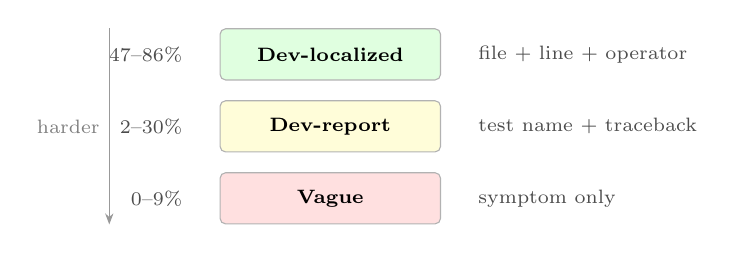
\begin{tikzpicture}[
  tier/.style={rectangle, rounded corners=2pt, minimum width=2.8cm,
    minimum height=0.65cm, font=\scriptsize\bfseries, align=center,
    draw=black!30, line width=0.4pt},
  ann/.style={font=\scriptsize, text=black!70, align=left},
  node distance=0.25cm
]

\node[tier, fill=green!12] (dl)
  {Dev-localized};
\node[tier, fill=yellow!15, below=of dl] (dr)
  {Dev-report};
\node[tier, fill=red!12, below=of dr] (vg)
  {Vague};

% Right: query content
\node[ann, right=0.35cm of dl] {file + line + operator};
\node[ann, right=0.35cm of dr] {test name + traceback};
\node[ann, right=0.35cm of vg] {symptom only};

% Left: pass@1 ranges
\node[ann, left=0.35cm of dl] {47--86\%};
\node[ann, left=0.35cm of dr] {2--30\%};
\node[ann, left=0.35cm of vg] {0--9\%};

% Arrow showing difficulty
\draw[-{Stealth[length=4pt]}, black!40]
  ([xshift=-1.4cm]dl.north west) -- ([xshift=-1.4cm]vg.south west)
  node[midway, left, font=\scriptsize, text=black!50] {harder};

\end{tikzpicture}
\caption{Three-tier query gradient with pass@1 ranges (non-ceiling methods).}
\label{fig:tier-gradient}
\end{figure}

\subsection{Methods}\label{sec:methods}

We evaluate ten retrieval methods plus a privileged ceiling
(\Cref{tab:methods}).

\begin{table}[tbp]
\centering
\caption{Retrieval methods.}\label{tab:methods}
\smallskip
\resizebox{\columnwidth}{!}{%
\begin{tabular}{lp{4.5cm}}
\toprule
Method & Description \\
\midrule
\textsc{no\_retrieval} & No context; query only \\
\textsc{bm25}          & BM25 keyword search~\citep{robertson1995okapi,robertson2009bm25} \\
\textsc{tfidf}        & TF-IDF cosine similarity~\citep{sparckjones1972,saltonbuckley1988} \\
\textsc{embedding}    & Dense embedding cosine similarity (\texttt{text-embedding-3-small}) \\
\textsc{keyword\_map}     & Repo file tree + keyword-matched symbol snippets (AST index) \\
\textsc{bca} ($d$=3)   & Graph BFS, depth 3, scoring + closure \\
\textsc{bca\_d1} ($d$=1) & BCA, depth 1 (shallow) \\
\textsc{bca\_d5} ($d$=5) & BCA, depth 5 (deep) \\
\textsc{bca\_no\_closure} & BCA without dep.\ closure \\
\textsc{bca\_no\_scoring} & BCA without scoring \\
\textsc{target\_file}  & Ceiling: mutated file given \\
\bottomrule
\end{tabular}%
}
\end{table}

The five BCA variants form an ablation study isolating the contribution
of expansion depth, dependency closure, and relevance scoring.

\smallskip
\noindent\textbf{Note on \textsc{keyword\_map}.}
\textsc{keyword\_map} is a simple, repository-local baseline that indexes file paths and
symbol signatures, then retrieves snippets via keyword matching.  In our released
artifacts and codebase, this method is keyed as \texttt{repo\_map}; we use the
\textsc{keyword\_map} name in the paper to avoid confusion with embedding-based ``vector
search'' and with Aider's repo-map algorithm.

\subsection{Evaluation Protocol}\label{sec:protocol}

\begin{itemize}[leftmargin=*,nosep]
  \item \textbf{Model:} \texttt{gpt-4o-mini-2024-07-18} (pinned snapshot)
  \item \textbf{Generation:} Single-shot (pass@1), temperature=0, seed=42
  \item \textbf{Budgets:} 2{,}000;\ 4{,}000;\ 8{,}000;\ 10{,}000 context tokens
    (estimated with \texttt{TokenEstimator}, 1~token $\approx$ 4~chars; LLM tokens from API usage)
  \item \textbf{Token accounting:} Budget enforcement uses the estimator during packing
    (\texttt{tokens\_used}).  We also log actual API prompt token counts
    (\texttt{llm\_input\_tokens}) and audit estimator error post-hoc
    (Appendix~\ref{app:token-audit}).
  \item \textbf{Total attempts:}
    245 tasks $\times$ 11~methods $\times$ 4~budgets $\times$ 3~tiers
    $= \mathbf{32{,}340}$
  \item \textbf{Success criterion:} Oracle test passes on patched code
  \item \textbf{Isolation:} Byte-identical file restoration between tasks (SHA-256 verified)
  \item \textbf{Bootstrap CIs:} task-resampled, $n$=5{,}000, seed=42~\citep{efron1993bootstrap}
\end{itemize}

% ══════════════════════════════════════════════════════════════════════════════
\section{Graph-Guided Baseline: BCA}\label{sec:bca}

We include BCA (Budgeted Context Assembly) as a graph-guided baseline
whose modular pipeline enables systematic ablation of individual
components.  BCA assembles context through eight phases
(\Cref{fig:bca-pipeline}):

\begin{figure*}[tbp]
\centering
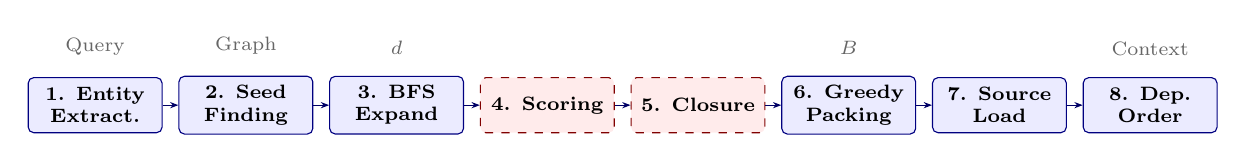
\begin{tikzpicture}[
  phase/.style={rectangle, rounded corners=2pt, draw=blue!50!black, fill=blue!8,
    minimum width=1.7cm, minimum height=0.7cm, font=\scriptsize\bfseries,
    align=center, line width=0.4pt},
  arrow/.style={-{Stealth[length=3pt]}, blue!40!black},
  plabel/.style={font=\scriptsize, text=black!60, align=center},
  node distance=0.3cm and 0.2cm
]

% Phase boxes in a single row
\node[phase] (p1) {1. Entity\\Extract.};
\node[phase, right=of p1] (p2) {2. Seed\\Finding};
\node[phase, right=of p2] (p3) {3. BFS\\Expand};
\node[phase, right=of p3, draw=red!50!black, fill=red!8, dashed] (p4) {4. Scoring};
\node[phase, right=of p4, draw=red!50!black, fill=red!8, dashed] (p5) {5. Closure};
\node[phase, right=of p5] (p6) {6. Greedy\\Packing};
\node[phase, right=of p6] (p7) {7. Source\\Load};
\node[phase, right=of p7] (p8) {8. Dep.\\Order};

% Arrows
\draw[arrow] (p1) -- (p2);
\draw[arrow] (p2) -- (p3);
\draw[arrow] (p3) -- (p4);
\draw[arrow] (p4) -- (p5);
\draw[arrow] (p5) -- (p6);
\draw[arrow] (p6) -- (p7);
\draw[arrow] (p7) -- (p8);

% Input/output labels
\node[plabel, above=0.15cm of p1] {Query};
\node[plabel, above=0.15cm of p2] {Graph};
\node[plabel, above=0.15cm of p3] {$d$};
\node[plabel, above=0.15cm of p6] {$B$};
\node[plabel, above=0.15cm of p8] {Context};


\end{tikzpicture}
\caption{The eight-phase BCA pipeline. Phases 4 and 5 are independently ablated to measure the contribution of relevance scoring and dependency closure.}
\label{fig:bca-pipeline}
\end{figure*}

\begin{enumerate}[leftmargin=*,nosep]
  \item \textbf{Entity extraction.}  Parse the query for code
 identifiers (function names, class names, module paths) using
    regex-based pattern matching.
  \item \textbf{Seed finding.}  Resolve extracted entities to symbols in the
    code knowledge graph (built from Python AST, capturing function/class
    definitions, imports, and call relationships).  When entity matching
    yields too few high-confidence seeds, we inject additional seeds using
    BM25 scoring over symbol metadata.
  \item \textbf{BFS expansion.}  Weighted breadth-first search from seeds
    to depth~$d$ over typed graph edges (calls/imports/contains/inherits/etc.),
    optionally including callers (predecessor edges).  Edge weights encode
    structural proximity and a minimum score threshold prunes the frontier.
  \item \textbf{Relevance scoring.}  Re-rank candidates with a seed-file
    proximity boost and a degree-centrality bonus, and penalize very large
    symbols.
  \item \textbf{Dependency closure.}  Add transitive hard dependencies
    (\texttt{inherits}/\texttt{implements}) and, for methods/functions, their
    containing class (optional; evaluated in ablation).
  \item \textbf{Greedy packing.}  Select highest-scoring symbols that fit
    within the token budget using a value-per-cost heuristic.  When closure
    dependencies are too expensive to include at full detail, we may include
    them as skeletons (signature + docstring only) to preserve interfaces
    under budget.
  \item \textbf{Source loading.}  Read actual source code for selected
    symbols from the repository, then enforce the budget using estimated token
    counts.  If the selected context underutilizes the budget, we backfill
    with BM25-ranked symbols and (if needed) keyword-matched files.
  \item \textbf{Dependency ordering.}  Sort context in topological order for
    the LLM.
\end{enumerate}

The code knowledge graph is built from Python AST parsing and captures
function definitions, class definitions, imports, and call relationships.
Graph construction takes approximately 2~seconds for pydantic-ai (186~files,
53k~lines).

Three depth strategies are evaluated (\Cref{tab:strategies}).

\begin{table}[tbp]
\centering
\caption{BCA depth strategies.}\label{tab:strategies}
\smallskip
\resizebox{\columnwidth}{!}{%
\begin{tabular}{lccc}
\toprule
Strategy & Depth & Min Score & Rationale \\
\midrule
\textsc{precise} (\textsc{bca\_d1}) & 1 & 0.3 & Immediate neighbors \\
\textsc{smart} (\textsc{bca})       & 3 & 0.1 & Default; balanced \\
\textsc{thorough} (\textsc{bca\_d5}) & 5 & 0.05 & Wide neighborhood \\
\bottomrule
\end{tabular}%
}
\end{table}

% ══════════════════════════════════════════════════════════════════════════════
\section{Results}\label{sec:results}

\subsection{Main Results}\label{sec:main-results}

Tables~\ref{tab:exact}--\ref{tab:vague} report pass@1 for all methods
across the three query tiers at all four budgets.  We report 95\% bootstrap
confidence intervals over tasks ($n$=5{,}000, seed=42) alongside point estimates.
\Cref{fig:main-heatmaps} provides a compact heatmap view of the same data.

% ── Table: Dev-localized ─────────────────────────────────────────────────────
\begin{table*}[tbp]
\centering
\caption{Pass@1 on \textbf{dev-localized} queries (95\% bootstrap CI).}\label{tab:exact}
\smallskip
\resizebox{\textwidth}{!}{%
\begin{tabular}{l cccc c}
\toprule
Method & $\B{2\text{k}}$ & $\B{4\text{k}}$ & $\B{8\text{k}}$ & $\B{10\text{k}}$ & Avg \\
\midrule
\textsc{no\_retrieval}  & \textbf{0.86} {\scriptsize[.82,.90]} & \textbf{0.86} {\scriptsize[.82,.90]} & \textbf{0.86} {\scriptsize[.82,.90]} & \textbf{0.86} {\scriptsize[.82,.90]} & \textbf{0.86} \\
\textsc{embedding}     & 0.76 {\scriptsize[.71,.81]} & 0.77 {\scriptsize[.71,.82]} & 0.76 {\scriptsize[.71,.81]} & 0.80 {\scriptsize[.75,.85]} & 0.77 \\
\textsc{tfidf}         & 0.74 {\scriptsize[.69,.80]} & 0.74 {\scriptsize[.69,.80]} & 0.76 {\scriptsize[.71,.82]} & 0.79 {\scriptsize[.74,.84]} & 0.76 \\
\textsc{keyword\_map}      & 0.72 {\scriptsize[.66,.78]} & 0.73 {\scriptsize[.67,.78]} & 0.75 {\scriptsize[.69,.80]} & 0.75 {\scriptsize[.69,.80]} & 0.74 \\
\textsc{bm25}           & 0.70 {\scriptsize[.64,.76]} & 0.71 {\scriptsize[.65,.76]} & 0.73 {\scriptsize[.68,.79]} & 0.76 {\scriptsize[.71,.81]} & 0.72 \\
\textsc{bca\_no\_closure} & 0.56 {\scriptsize[.50,.62]} & 0.64 {\scriptsize[.58,.70]} & 0.69 {\scriptsize[.63,.75]} & 0.72 {\scriptsize[.67,.78]} & 0.65 \\
\textsc{bca} ($d$=3)     & 0.52 {\scriptsize[.46,.59]} & 0.64 {\scriptsize[.58,.70]} & 0.69 {\scriptsize[.64,.75]} & 0.69 {\scriptsize[.64,.75]} & 0.64 \\
\textsc{bca\_d5}        & 0.55 {\scriptsize[.49,.61]} & 0.64 {\scriptsize[.58,.69]} & 0.66 {\scriptsize[.60,.72]} & 0.69 {\scriptsize[.63,.75]} & 0.63 \\
\textsc{bca\_no\_scoring} & 0.48 {\scriptsize[.42,.54]} & 0.63 {\scriptsize[.57,.69]} & 0.67 {\scriptsize[.61,.73]} & 0.66 {\scriptsize[.60,.72]} & 0.61 \\
\textsc{bca\_d1}        & 0.47 {\scriptsize[.40,.53]} & 0.53 {\scriptsize[.47,.60]} & 0.65 {\scriptsize[.60,.71]} & 0.69 {\scriptsize[.63,.74]} & 0.58 \\
\midrule
Oracle                  & 0.97 & 0.98 & 0.97 & 0.98 & 0.97 \\
\bottomrule
\end{tabular}%
}
\end{table*}

% ── Heatmap: Main pass@1 across tiers ────────────────────────────────────────
\begin{figure*}[tbp]
\centering
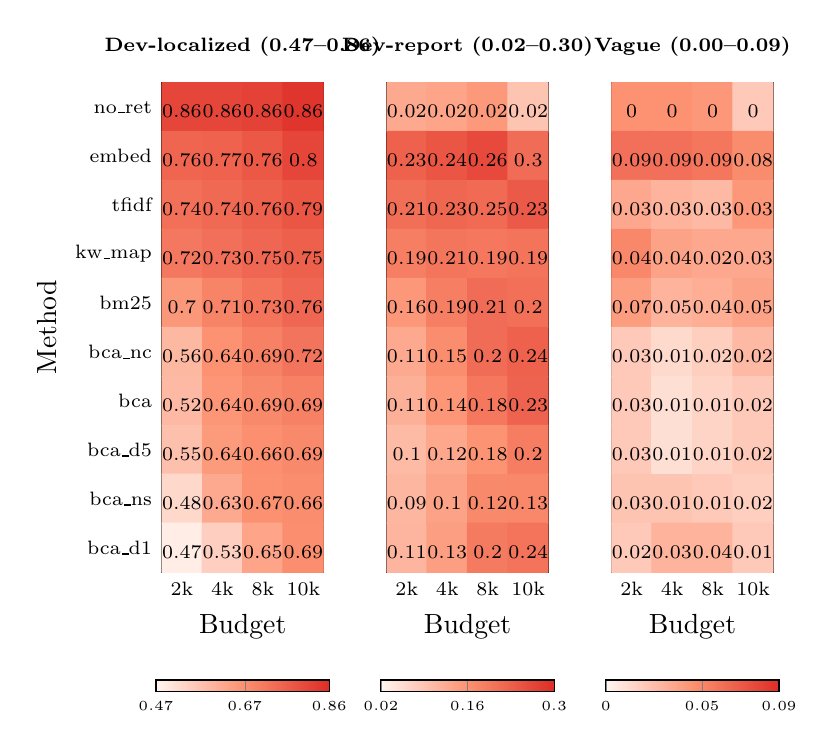
\begin{tikzpicture}
\begin{groupplot}[
  group style={group size=3 by 1, horizontal sep=0.8cm},
  width=0.30\textwidth,
  height=7.8cm,
  y dir=reverse,
  xmin=-0.5, xmax=3.5,
  ymin=-0.5, ymax=9.5,
  xtick={0,1,2,3},
  xticklabels={2k,4k,8k,10k},
  ytick={0,1,2,3,4,5,6,7,8,9},
  yticklabels={no\_ret,embed,tfidf,kw\_map,bm25,bca\_nc,bca,bca\_d5,bca\_ns,bca\_d1},
  xlabel={Budget},
  colormap={hm}{rgb255=(255,245,240) rgb255=(252,146,114) rgb255=(222,45,38)},
  nodes near coords,
  every axis plot/.append style={draw=white, line width=0.45pt},
  every node near coord/.append style={
    font=\scriptsize,
    /pgf/number format/fixed,
    /pgf/number format/precision=2,
    text=black,
    anchor=center,
    yshift=-0.35ex
  },
  tick label style={font=\scriptsize},
  title style={font=\scriptsize\bfseries},
]
\nextgroupplot[
  title={Dev-localized (0.47--0.86)},
  ylabel={Method},
  point meta min=0.47,
  point meta max=0.86,
  colorbar horizontal,
  colorbar style={
    at={(0.5,-0.22)},
    anchor=north,
    width=2.2cm,
    height=1.5mm,
    xticklabel style={font=\tiny},
    xtick={0.47,0.67,0.86},
    scaled x ticks=false,
    every node near coord/.style={text opacity=0},
  }
]
\addplot[
  matrix plot*,
  shader=flat,
  mesh/cols=4,
  point meta=explicit,
] coordinates {
  (0,0) [0.86] (1,0) [0.86] (2,0) [0.86] (3,0) [0.86]
  (0,1) [0.76] (1,1) [0.77] (2,1) [0.76] (3,1) [0.80]
  (0,2) [0.74] (1,2) [0.74] (2,2) [0.76] (3,2) [0.79]
  (0,3) [0.72] (1,3) [0.73] (2,3) [0.75] (3,3) [0.75]
  (0,4) [0.70] (1,4) [0.71] (2,4) [0.73] (3,4) [0.76]
  (0,5) [0.56] (1,5) [0.64] (2,5) [0.69] (3,5) [0.72]
  (0,6) [0.52] (1,6) [0.64] (2,6) [0.69] (3,6) [0.69]
  (0,7) [0.55] (1,7) [0.64] (2,7) [0.66] (3,7) [0.69]
  (0,8) [0.48] (1,8) [0.63] (2,8) [0.67] (3,8) [0.66]
  (0,9) [0.47] (1,9) [0.53] (2,9) [0.65] (3,9) [0.69]
};

\nextgroupplot[
  title={Dev-report (0.02--0.30)},
  yticklabels={},
  point meta min=0.02,
  point meta max=0.30,
  colorbar horizontal,
  colorbar style={
    at={(0.5,-0.22)},
    anchor=north,
    width=2.2cm,
    height=1.5mm,
    xticklabel style={font=\tiny},
    xtick={0.02,0.16,0.30},
    scaled x ticks=false,
    every node near coord/.style={text opacity=0},
  }
]
\addplot[
  matrix plot*,
  shader=flat,
  mesh/cols=4,
  point meta=explicit,
] coordinates {
  (0,0) [0.02] (1,0) [0.02] (2,0) [0.02] (3,0) [0.02]
  (0,1) [0.23] (1,1) [0.24] (2,1) [0.26] (3,1) [0.30]
  (0,2) [0.21] (1,2) [0.23] (2,2) [0.25] (3,2) [0.23]
  (0,3) [0.19] (1,3) [0.21] (2,3) [0.19] (3,3) [0.19]
  (0,4) [0.16] (1,4) [0.19] (2,4) [0.21] (3,4) [0.20]
  (0,5) [0.11] (1,5) [0.15] (2,5) [0.20] (3,5) [0.24]
  (0,6) [0.11] (1,6) [0.14] (2,6) [0.18] (3,6) [0.23]
  (0,7) [0.10] (1,7) [0.12] (2,7) [0.18] (3,7) [0.20]
  (0,8) [0.09] (1,8) [0.10] (2,8) [0.12] (3,8) [0.13]
  (0,9) [0.11] (1,9) [0.13] (2,9) [0.20] (3,9) [0.24]
};

\nextgroupplot[
  title={Vague (0.00--0.09)},
  yticklabels={},
  point meta min=0.00,
  point meta max=0.09,
  colorbar horizontal,
  colorbar style={
    at={(0.5,-0.22)},
    anchor=north,
    width=2.2cm,
    height=1.5mm,
    xticklabel style={font=\tiny},
    xtick={0.00,0.05,0.09},
    scaled x ticks=false,
    every node near coord/.style={text opacity=0},
  }
]
\addplot[
  matrix plot*,
  shader=flat,
  mesh/cols=4,
  point meta=explicit,
] coordinates {
  (0,0) [0.00] (1,0) [0.00] (2,0) [0.00] (3,0) [0.00]
  (0,1) [0.09] (1,1) [0.09] (2,1) [0.09] (3,1) [0.08]
  (0,2) [0.03] (1,2) [0.03] (2,2) [0.03] (3,2) [0.03]
  (0,3) [0.04] (1,3) [0.04] (2,3) [0.02] (3,3) [0.03]
  (0,4) [0.07] (1,4) [0.05] (2,4) [0.04] (3,4) [0.05]
  (0,5) [0.03] (1,5) [0.01] (2,5) [0.02] (3,5) [0.02]
  (0,6) [0.03] (1,6) [0.01] (2,6) [0.01] (3,6) [0.02]
  (0,7) [0.03] (1,7) [0.01] (2,7) [0.01] (3,7) [0.02]
  (0,8) [0.03] (1,8) [0.01] (2,8) [0.01] (3,8) [0.02]
  (0,9) [0.02] (1,9) [0.03] (2,9) [0.04] (3,9) [0.01]
};
\end{groupplot}
\end{tikzpicture}
\caption{Pass@1 heatmaps for the three query tiers (methods $\times$ budgets). Each panel uses its own color scale (colorbars below) to make within-tier ranking patterns readable; exact values remain in Tables~\ref{tab:exact}--\ref{tab:vague}.}
\label{fig:main-heatmaps}
\end{figure*}

\begin{figure*}[tbp]
\centering
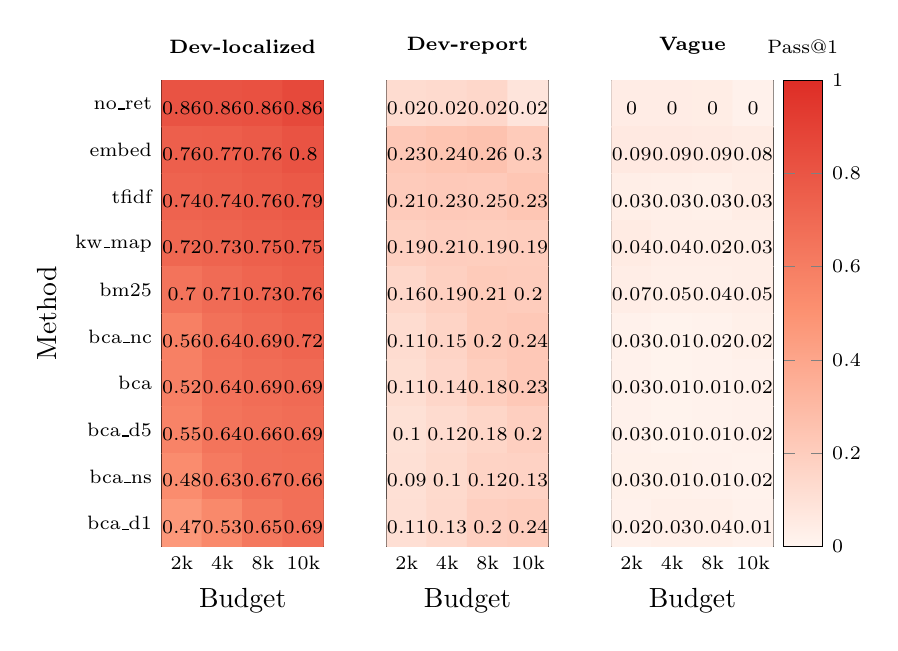
\begin{tikzpicture}
\begin{groupplot}[
  group style={group size=3 by 1, horizontal sep=0.8cm},
  width=0.30\textwidth,
  height=7.5cm,
  y dir=reverse,
  xmin=-0.5, xmax=3.5,
  ymin=-0.5, ymax=9.5,
  xtick={0,1,2,3},
  xticklabels={2k,4k,8k,10k},
  ytick={0,1,2,3,4,5,6,7,8,9},
  yticklabels={no\_ret,embed,tfidf,kw\_map,bm25,bca\_nc,bca,bca\_d5,bca\_ns,bca\_d1},
  xlabel={Budget},
  point meta min=0.00,
  point meta max=1.00,
  colormap={hmglobal}{rgb255=(255,245,240) rgb255=(252,146,114) rgb255=(222,45,38)},
  nodes near coords,
  every axis plot/.append style={draw=white, line width=0.45pt},
  every node near coord/.append style={
    font=\scriptsize,
    /pgf/number format/fixed,
    /pgf/number format/precision=2,
    text=black,
    anchor=center,
    yshift=-0.35ex
  },
  tick label style={font=\scriptsize},
  title style={font=\scriptsize\bfseries},
]
\nextgroupplot[title={Dev-localized}, ylabel={Method}]
\addplot[
  matrix plot*,
  shader=flat,
  mesh/cols=4,
  point meta=explicit,
] coordinates {
  (0,0) [0.86] (1,0) [0.86] (2,0) [0.86] (3,0) [0.86]
  (0,1) [0.76] (1,1) [0.77] (2,1) [0.76] (3,1) [0.80]
  (0,2) [0.74] (1,2) [0.74] (2,2) [0.76] (3,2) [0.79]
  (0,3) [0.72] (1,3) [0.73] (2,3) [0.75] (3,3) [0.75]
  (0,4) [0.70] (1,4) [0.71] (2,4) [0.73] (3,4) [0.76]
  (0,5) [0.56] (1,5) [0.64] (2,5) [0.69] (3,5) [0.72]
  (0,6) [0.52] (1,6) [0.64] (2,6) [0.69] (3,6) [0.69]
  (0,7) [0.55] (1,7) [0.64] (2,7) [0.66] (3,7) [0.69]
  (0,8) [0.48] (1,8) [0.63] (2,8) [0.67] (3,8) [0.66]
  (0,9) [0.47] (1,9) [0.53] (2,9) [0.65] (3,9) [0.69]
};

\nextgroupplot[title={Dev-report}, yticklabels={}]
\addplot[
  matrix plot*,
  shader=flat,
  mesh/cols=4,
  point meta=explicit,
] coordinates {
  (0,0) [0.02] (1,0) [0.02] (2,0) [0.02] (3,0) [0.02]
  (0,1) [0.23] (1,1) [0.24] (2,1) [0.26] (3,1) [0.30]
  (0,2) [0.21] (1,2) [0.23] (2,2) [0.25] (3,2) [0.23]
  (0,3) [0.19] (1,3) [0.21] (2,3) [0.19] (3,3) [0.19]
  (0,4) [0.16] (1,4) [0.19] (2,4) [0.21] (3,4) [0.20]
  (0,5) [0.11] (1,5) [0.15] (2,5) [0.20] (3,5) [0.24]
  (0,6) [0.11] (1,6) [0.14] (2,6) [0.18] (3,6) [0.23]
  (0,7) [0.10] (1,7) [0.12] (2,7) [0.18] (3,7) [0.20]
  (0,8) [0.09] (1,8) [0.10] (2,8) [0.12] (3,8) [0.13]
  (0,9) [0.11] (1,9) [0.13] (2,9) [0.20] (3,9) [0.24]
};

\nextgroupplot[
  title={Vague},
  yticklabels={},
  colorbar,
  colorbar style={
    title={Pass@1},
    title style={font=\scriptsize},
    at={(1.06,0.5)},
    anchor=west,
    yticklabel style={font=\scriptsize},
    scaled y ticks=false,
    y dir=normal,
    every node near coord/.style={text opacity=0},
  }
]
\addplot[
  matrix plot*,
  shader=flat,
  mesh/cols=4,
  point meta=explicit,
] coordinates {
  (0,0) [0.00] (1,0) [0.00] (2,0) [0.00] (3,0) [0.00]
  (0,1) [0.09] (1,1) [0.09] (2,1) [0.09] (3,1) [0.08]
  (0,2) [0.03] (1,2) [0.03] (2,2) [0.03] (3,2) [0.03]
  (0,3) [0.04] (1,3) [0.04] (2,3) [0.02] (3,3) [0.03]
  (0,4) [0.07] (1,4) [0.05] (2,4) [0.04] (3,4) [0.05]
  (0,5) [0.03] (1,5) [0.01] (2,5) [0.02] (3,5) [0.02]
  (0,6) [0.03] (1,6) [0.01] (2,6) [0.01] (3,6) [0.02]
  (0,7) [0.03] (1,7) [0.01] (2,7) [0.01] (3,7) [0.02]
  (0,8) [0.03] (1,8) [0.01] (2,8) [0.01] (3,8) [0.02]
  (0,9) [0.02] (1,9) [0.03] (2,9) [0.04] (3,9) [0.01]
};
\end{groupplot}
\end{tikzpicture}
\caption{Pass@1 heatmaps with a shared global color scale (0.00--1.00). Unlike \Cref{fig:main-heatmaps}, colors are directly comparable across tiers; dev-report and vague cells compress near the low end.}
\label{fig:main-heatmaps-global}
\end{figure*}

\paragraph{Interpreting the two heatmap views.}
\Cref{fig:main-heatmaps} is for \emph{within-tier ranking}: each panel rescales colors to highlight method ordering inside that tier.
\Cref{fig:main-heatmaps-global} is for \emph{cross-tier magnitude}: the shared color scale makes the dev-localized \(\rightarrow\) dev-report \(\rightarrow\) vague collapse visually explicit.
Taken together, they show both facts at once: rankings can shift with budget inside a tier, but absolute performance is primarily determined by query tier.

% ── Table: Dev-report ────────────────────────────────────────────────────────
\begin{table*}[tbp]
\centering
\caption{Pass@1 on \textbf{dev-report} queries (95\% bootstrap CI).}\label{tab:devreport}
\smallskip
\resizebox{\textwidth}{!}{%
\begin{tabular}{l cccc c}
\toprule
Method & $\B{2\text{k}}$ & $\B{4\text{k}}$ & $\B{8\text{k}}$ & $\B{10\text{k}}$ & Avg \\
\midrule
\textsc{embedding}     & \textbf{0.23} {\scriptsize[.18,.29]} & \textbf{0.24} {\scriptsize[.18,.29]} & \textbf{0.26} {\scriptsize[.21,.32]} & \textbf{0.30} {\scriptsize[.24,.36]} & \textbf{0.26} \\
\textsc{tfidf}         & 0.21 {\scriptsize[.16,.27]} & 0.23 {\scriptsize[.18,.28]} & 0.25 {\scriptsize[.20,.31]} & 0.23 {\scriptsize[.18,.29]} & 0.23 \\
\textsc{keyword\_map}      & 0.19 {\scriptsize[.14,.24]} & 0.21 {\scriptsize[.16,.26]} & 0.19 {\scriptsize[.14,.24]} & 0.19 {\scriptsize[.14,.24]} & 0.19 \\
\textsc{bm25}           & 0.16 {\scriptsize[.12,.21]} & 0.19 {\scriptsize[.14,.24]} & 0.21 {\scriptsize[.16,.27]} & 0.20 {\scriptsize[.15,.24]} & 0.19 \\
\textsc{bca\_no\_closure} & 0.11 {\scriptsize[.07,.15]} & 0.15 {\scriptsize[.11,.19]} & 0.20 {\scriptsize[.15,.25]} & \textbf{0.24} {\scriptsize[.19,.30]} & 0.18 \\
\textsc{bca\_d1}        & 0.11 {\scriptsize[.07,.16]} & 0.13 {\scriptsize[.09,.17]} & 0.20 {\scriptsize[.16,.25]} & \textbf{0.24} {\scriptsize[.19,.30]} & 0.17 \\
\textsc{bca} ($d$=3)     & 0.11 {\scriptsize[.07,.15]} & 0.14 {\scriptsize[.10,.18]} & 0.18 {\scriptsize[.13,.23]} & 0.23 {\scriptsize[.18,.29]} & 0.16 \\
\textsc{bca\_d5}        & 0.10 {\scriptsize[.06,.14]} & 0.12 {\scriptsize[.08,.16]} & 0.18 {\scriptsize[.14,.24]} & 0.20 {\scriptsize[.16,.26]} & 0.15 \\
\textsc{bca\_no\_scoring} & 0.09 {\scriptsize[.06,.13]} & 0.10 {\scriptsize[.06,.14]} & 0.12 {\scriptsize[.08,.16]} & 0.13 {\scriptsize[.09,.18]} & 0.11 \\
\textsc{no\_retrieval}  & 0.02 {\scriptsize[.01,.04]} & 0.02 {\scriptsize[.01,.04]} & 0.02 {\scriptsize[.01,.04]} & 0.02 {\scriptsize[.01,.04]} & 0.02 \\
\midrule
Oracle                  & 0.40 & 0.43 & 0.48 & 0.49 & 0.45 \\
\bottomrule
\end{tabular}%
}
\end{table*}

% ── Table: Vague ─────────────────────────────────────────────────────────────
\begin{table*}[tbp]
\centering
\caption{Pass@1 on \textbf{vague} queries (95\% bootstrap CI).}\label{tab:vague}
\smallskip
\resizebox{\textwidth}{!}{%
\begin{tabular}{l cccc c}
\toprule
Method & $\B{2\text{k}}$ & $\B{4\text{k}}$ & $\B{8\text{k}}$ & $\B{10\text{k}}$ & Avg \\
\midrule
\textsc{embedding}     & \textbf{0.09} {\scriptsize[.06,.13]} & \textbf{0.09} {\scriptsize[.06,.13]} & \textbf{0.09} {\scriptsize[.06,.13]} & \textbf{0.08} {\scriptsize[.05,.12]} & \textbf{0.09} \\
\textsc{bm25}           & 0.07 {\scriptsize[.04,.10]} & 0.05 {\scriptsize[.02,.08]} & 0.04 {\scriptsize[.02,.07]} & 0.05 {\scriptsize[.03,.09]} & 0.05 \\
\textsc{keyword\_map}      & 0.04 {\scriptsize[.02,.06]} & 0.04 {\scriptsize[.02,.06]} & 0.02 {\scriptsize[.01,.04]} & 0.03 {\scriptsize[.01,.05]} & 0.03 \\
\textsc{tfidf}         & 0.03 {\scriptsize[.01,.06]} & 0.03 {\scriptsize[.01,.05]} & 0.03 {\scriptsize[.01,.05]} & 0.03 {\scriptsize[.01,.05]} & 0.03 \\
\textsc{bca} ($d$=3)     & 0.03 {\scriptsize[.01,.05]} & 0.01 {\scriptsize[.00,.03]} & 0.01 {\scriptsize[.00,.02]} & 0.02 {\scriptsize[.00,.04]} & 0.02 \\
\textsc{bca\_d1}        & 0.02 {\scriptsize[.00,.03]} & 0.03 {\scriptsize[.01,.05]} & \textbf{0.04} {\scriptsize[.02,.06]} & 0.01 {\scriptsize[.00,.03]} & 0.02 \\
\textsc{bca\_d5}        & 0.03 {\scriptsize[.01,.05]} & 0.01 {\scriptsize[.00,.03]} & 0.01 {\scriptsize[.00,.03]} & 0.02 {\scriptsize[.00,.03]} & 0.02 \\
\textsc{bca\_no\_closure} & 0.03 {\scriptsize[.01,.05]} & 0.01 {\scriptsize[.00,.02]} & 0.02 {\scriptsize[.00,.03]} & 0.02 {\scriptsize[.00,.03]} & 0.02 \\
\textsc{bca\_no\_scoring} & 0.03 {\scriptsize[.01,.06]} & 0.01 {\scriptsize[.00,.02]} & 0.01 {\scriptsize[.00,.03]} & 0.02 {\scriptsize[.00,.03]} & 0.02 \\
\textsc{no\_retrieval}  & 0.00 {\scriptsize[.00,.00]} & 0.00 {\scriptsize[.00,.00]} & 0.00 {\scriptsize[.00,.00]} & 0.00 {\scriptsize[.00,.00]} & 0.00 \\
\midrule
Oracle                  & 0.14 & 0.12 & 0.12 & 0.11 & 0.12 \\
\bottomrule
\end{tabular}%
}
\end{table*}

% ── Chart: Dev-report pass@1 by method across budgets ────────────────────────
\begin{figure*}[tbp]
\centering
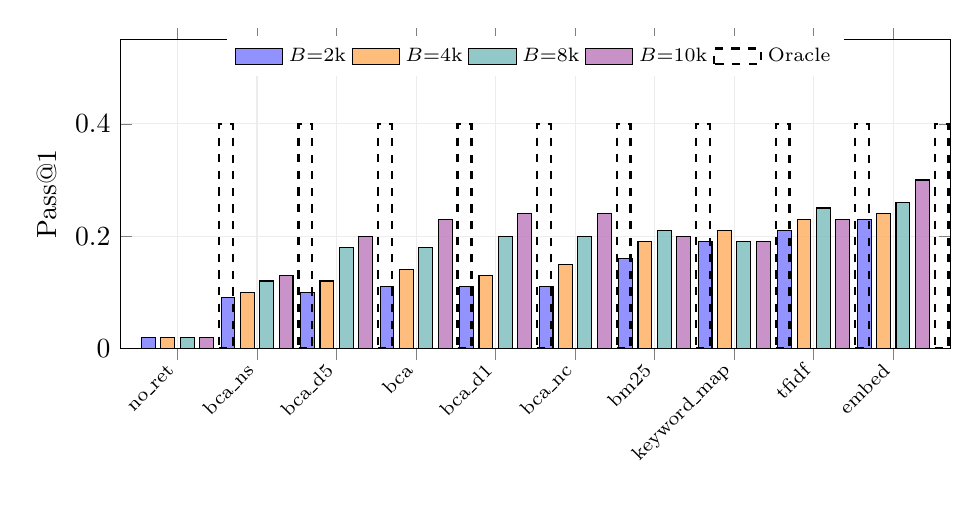
\begin{tikzpicture}
\begin{axis}[
    ybar,
    area legend,
    bar width=5pt,
    width=\textwidth,
    height=5.5cm,
    ylabel={Pass@1},
    symbolic x coords={no\_ret, bca\_ns, bca\_d5, bca, bca\_d1, bca\_nc, bm25, keyword\_map, tfidf, embed},
    xtick=data,
    x tick label style={rotate=45, anchor=east, font=\scriptsize},
    ymin=0, ymax=0.55,
    legend style={
      font=\scriptsize,
      legend columns=5,
      draw=none,
      at={(0.5,0.88)},
      anchor=south
    },
    enlarge x limits=0.08,
    grid=major,
    grid style={gray!15},
    every axis plot/.append style={fill opacity=0.85},
]
\addplot[fill=blue!50] coordinates {(no\_ret,0.02) (bca\_ns,0.09) (bca\_d5,0.10) (bca,0.11) (bca\_d1,0.11) (bca\_nc,0.11) (bm25,0.16) (keyword\_map,0.19) (tfidf,0.21) (embed,0.23)};
\addlegendentry{$B$=2k}
\addplot[fill=orange!60] coordinates {(no\_ret,0.02) (bca\_ns,0.10) (bca\_d5,0.12) (bca,0.14) (bca\_d1,0.13) (bca\_nc,0.15) (bm25,0.19) (keyword\_map,0.21) (tfidf,0.23) (embed,0.24)};
\addlegendentry{$B$=4k}
\addplot[fill=teal!50] coordinates {(no\_ret,0.02) (bca\_ns,0.12) (bca\_d5,0.18) (bca,0.18) (bca\_d1,0.20) (bca\_nc,0.20) (bm25,0.21) (keyword\_map,0.19) (tfidf,0.25) (embed,0.26)};
\addlegendentry{$B$=8k}
\addplot[fill=violet!50] coordinates {(no\_ret,0.02) (bca\_ns,0.13) (bca\_d5,0.20) (bca,0.23) (bca\_d1,0.24) (bca\_nc,0.24) (bm25,0.20) (keyword\_map,0.19) (tfidf,0.23) (embed,0.30)};
\addlegendentry{$B$=10k}
\addplot[black, thick, dashed, mark=none, forget plot]
    coordinates {(no\_ret,0.40) (bca\_ns,0.40) (bca\_d5,0.40) (bca,0.40) (bca\_d1,0.40) (bca\_nc,0.40) (bm25,0.40) (keyword\_map,0.40) (tfidf,0.40) (embed,0.40)};
\addlegendimage{black, thick, dashed}
\addlegendentry{Oracle}
\end{axis}
\end{tikzpicture}\\[4pt]
\caption{Dev-report pass@1 by method across four token budgets. Methods sorted by $\B{2\text{k}}$ performance. Horizontal marks show the per-task oracle at $\B{2\text{k}}$ (0.40). Dense embedding leads at all budgets.}
\label{fig:devreport-bars}
\end{figure*}

% ── Chart: Budget scaling lines for dev-report ───────────────────────────────
\begin{figure}[tbp]
\centering
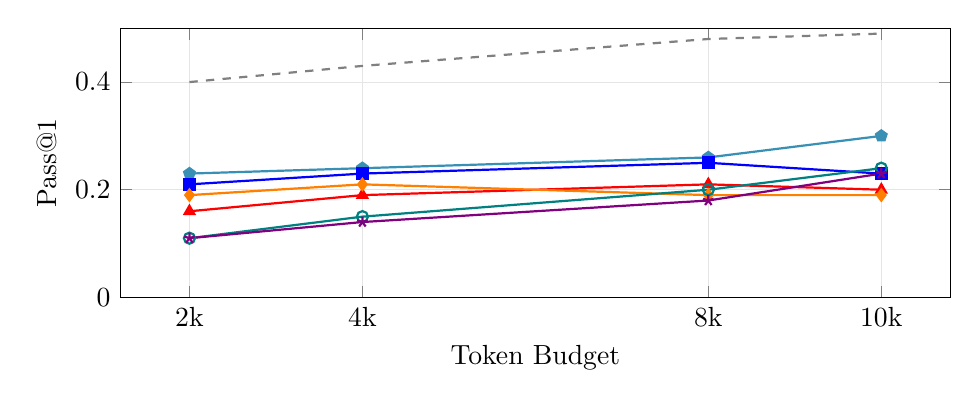
\begin{tikzpicture}
\begin{axis}[
    width=\columnwidth,
    height=5cm,
    xlabel={Token Budget},
    ylabel={Pass@1},
    xtick={2000,4000,8000,10000},
    xticklabels={2k,4k,8k,10k},
    ymin=0, ymax=0.50,
    legend to name=leg:budgetscale,
    legend style={font=\scriptsize, legend columns=3, draw=none},
    grid=major,
    grid style={gray!20},
    every axis plot/.append style={thick, mark size=2pt},
]
\addplot[cyan!70!black, mark=pentagon*, thick] coordinates {(2000,0.23) (4000,0.24) (8000,0.26) (10000,0.30)};
\addplot[blue, mark=square*] coordinates {(2000,0.21) (4000,0.23) (8000,0.25) (10000,0.23)};
\addplot[red, mark=triangle*] coordinates {(2000,0.16) (4000,0.19) (8000,0.21) (10000,0.20)};
\addplot[orange, mark=diamond*] coordinates {(2000,0.19) (4000,0.21) (8000,0.19) (10000,0.19)};
\addplot[teal, mark=o] coordinates {(2000,0.11) (4000,0.15) (8000,0.20) (10000,0.24)};
\addplot[violet, mark=star] coordinates {(2000,0.11) (4000,0.14) (8000,0.18) (10000,0.23)};
\addplot[gray, dashed, mark=none] coordinates {(2000,0.40) (4000,0.43) (8000,0.48) (10000,0.49)};
\legend{embedding, tfidf, bm25, keyword\_map, bca\_nc, bca, oracle}
\end{axis}
\end{tikzpicture}\\[4pt]
\ref{leg:budgetscale}
\caption{Dev-report pass@1 vs.\ token budget for selected methods. Method rankings shift at higher budgets, with graph-guided variants narrowing the gap with lexical methods.}
\label{fig:budget-scaling}
\end{figure}

\subsection{The Three-Tier Gradient}\label{sec:gradient}

Across all methods and budgets we evaluated, pass@1 decreases monotonically
from dev-localized to dev-report to vague.

\paragraph{Dev-localized queries trivialize the task.}
\textsc{no\_retrieval} achieves 86\% pass@1: the LLM fixes bugs from the
description alone because the query leaks the file, line number, and
operator change.  Adding retrieval context actually reduces performance for
all methods, consistent with extra context acting as noise when the edit
location is already specified in the query.

\paragraph{Dev-report is the meaningful evaluation tier.}
Methods score 9--30\%.  The traceback provides enough signal for retrieval
(function names, test names, error messages) but not enough for the LLM to
fix without code context.  \textsc{no\_retrieval} drops to 2\%, confirming
that context is essential.

\paragraph{Vague queries expose a model bottleneck.}
All methods score 0--9\%.  The ceiling probe (\Cref{sec:ceiling}) shows that
even with the \emph{correct file}, the LLM only fixes 30\% of tasks from
vague descriptions.  The bottleneck is model comprehension, not retrieval
quality.

\paragraph{Method rankings shift with budget.}
At $\B{2\text{k}}$, BCA~(0.11) trails embedding~(0.23) by 12 percentage
points.  At $\B{10\text{k}}$, \textsc{bca\_no\_closure} and
\textsc{bca\_d1}~(0.24) approach but do not match embedding~(0.30).
Dense embedding benefits from semantic matching of traceback terms to
symbol descriptions.  Graph-guided retrieval needs budget to include both
seed symbols and their dependency neighborhoods; at tight budgets, it
cannot fit enough context.

\subsection{Ceiling Analysis}\label{sec:ceiling}

The ceiling probe (\textsc{target\_file}) provides the mutated file as
context, establishing an upper bound on repair rate if retrieval were perfect
(\Cref{tab:ceiling}).

\begin{table}[tbp]
\centering
\caption{Ceiling analysis at $\B{10\text{k}}$: best single method vs.\ target file ceiling vs.\ oracle.}\label{tab:ceiling}
\smallskip
\resizebox{\columnwidth}{!}{%
\begin{tabular}{lcccc}
\toprule
Tier & Best Method & Ceiling & Oracle & Gap (Oracle--Best) \\
\midrule
Dev-loc. & 0.86 (\textsc{no\_retrieval}) & 0.92 & 0.98 & 12pp \\
Dev-rep. & 0.30 (\textsc{embedding}) & 0.48 & 0.49 & 19pp \\
Vague    & 0.08 (\textsc{embedding}) & 0.30 & 0.11 & 3pp \\
\bottomrule
\end{tabular}%
}
\end{table}

The dev-report ceiling~(0.48 at $\B{4\text{k}}$+) shows that even with the
perfect file, \texttt{gpt-4o-mini} fixes only 48\% of tasks from a
traceback.  The median target file is approximately 3{,}118~tokens, so the
ceiling saturates at $\B{4\text{k}}$.  On vague queries, the ceiling barely
improves with budget (0.24 at $\B{2\text{k}}$ to 0.30 at $\B{10\text{k}}$),
confirming that model comprehension is the bottleneck.

On dev-report, the oracle rises from 0.40 ($\B{2\text{k}}$) to 0.49
($\B{10\text{k}}$), converging with the ceiling~(0.48).  At lower budgets
the oracle falls below the ceiling because retrieval methods may miss the
target file; at $\B{10\text{k}}$ the oracle marginally exceeds the ceiling,
indicating that some tasks benefit from multi-file context that no single
target file provides.

% ══════════════════════════════════════════════════════════════════════════════

% ── Worked Example ────────────────────────────────────────────────────────────
\begin{figure*}[tbp]
\centering
\small
\setlength{\tabcolsep}{4pt}
\begin{tabular}{@{}p{0.48\textwidth}p{0.48\textwidth}@{}}
\toprule
\multicolumn{2}{c}{\textbf{Worked Example: \texttt{usage-total-tokens-math}} ($\B{4\text{k}}$, dev-report)} \\
\midrule
\multicolumn{2}{l}{\textbf{Mutation:} \texttt{usage.py:66} \quad \texttt{input\_tokens + output\_tokens} $\to$ \texttt{input\_tokens - output\_tokens}} \\[4pt]
\multicolumn{2}{l}{\textbf{Dev-localized:} ``\texttt{usage.py} line 66: \texttt{+} replaced with \texttt{-} in \texttt{total\_tokens}.''} \\
\multicolumn{2}{l}{\textbf{Dev-report:} ``Test failure: \texttt{test\_total\_token\_limit}. \texttt{DID NOT RAISE UsageLimitExceeded}.''} \\
\multicolumn{2}{l}{\textbf{Vague:} ``Token usage tracking seems off. The total count is always lower than expected.''} \\
\midrule
\textbf{TF-IDF context} (44 symbols, 40 files) & \textbf{BCA context} (22 symbols, 4 files) \\
\midrule
Retrieves broadly: test file, exception class, & Retrieves via graph: \texttt{UsageLimitExceeded} $\to$ \\
13 unrelated test modules, 40 scattered files. & \texttt{usage.py} (contains mutation) $\to$ \\
Target file hit: \checkmark \quad Target symbol hit: \checkmark & \texttt{test\_usage\_limits.py} (4 focused files). \\
Context--patch overlap: 0.025 & Context--patch overlap: 0.25 \\
\midrule
\textbf{Patch:} \texttt{- $\to$ +} \quad \checkmark~Pass & \textbf{Patch:} \texttt{- $\to$ +} \quad \checkmark~Pass \\
\bottomrule
\end{tabular}
\caption{End-to-end walkthrough of one dev-report task at $\B{4\text{k}}$.
TF-IDF spreads its budget across 40 files with low overlap (0.025); BCA concentrates on 4 graph-connected files with 10$\times$ higher overlap (0.25).
Both produce the correct single-line fix.
This illustrates why pass@1 alone does not distinguish retrieval quality: structurally different contexts can yield identical outcomes.}
\label{fig:worked-example}
\end{figure*}

\section{Mechanistic Analysis}\label{sec:mechanistic}

\subsection{Failure Mode Gradient}\label{sec:failures}

We classify each attempt's outcome into one of five categories:
\emph{pass} (test suite passes),
\emph{patch\_apply\_fail} (patch does not apply cleanly),
\emph{test\_fail} (patch applies but tests fail),
\emph{syntax\_error} (generated code has syntax errors), and
\emph{timeout} (test execution exceeds the time limit).
Table~\ref{tab:fail-devreport-full} reports the full failure mode
distribution for dev-report (all methods and budgets).  For completeness,
the corresponding dev-localized and vague tables are provided in
Appendix~\ref{app:supp-tables} (Tables~\ref{tab:fail-exact-full} and
\ref{tab:fail-vague-full}).

\begin{table*}[tbp]
\centering
\caption{Failure mode distribution (\%), dev-report, all methods and budgets.}\label{tab:fail-devreport-full}
\smallskip
\resizebox{\textwidth}{!}{%
\begin{tabular}{l ccccc ccccc ccccc ccccc}
\toprule
& \multicolumn{5}{c}{$\B{2\text{k}}$}
& \multicolumn{5}{c}{$\B{4\text{k}}$}
& \multicolumn{5}{c}{$\B{8\text{k}}$}
& \multicolumn{5}{c}{$\B{10\text{k}}$} \\
\cmidrule(lr){2-6}\cmidrule(lr){7-11}\cmidrule(lr){12-16}\cmidrule(lr){17-21}
Method & pass & patch & test & syn & t/o
       & pass & patch & test & syn & t/o
       & pass & patch & test & syn & t/o
       & pass & patch & test & syn & t/o \\
\midrule
\textsc{bca}              & 11 & 22 & 62 & 1 & 4  & 14 & 24 & 57 & 3 & 2  & 18 & 27 & 49 & 3 & 2  & 23 & 21 & 49 & 3 & 4 \\
\textsc{bca\_d1}          & 11 & 22 & 60 & 2 & 4  & 13 & 22 & 55 & 7 & 4  & 20 & 21 & 52 & 3 & 3  & 24 & 16 & 49 & 7 & 4 \\
\textsc{bca\_d5}          & 10 & 24 & 61 & 2 & 3  & 12 & 31 & 51 & 5 & 2  & 18 & 25 & 51 & 3 & 2  & 20 & 24 & 49 & 4 & 3 \\
\textsc{bca\_no\_closure} & 11 & 24 & 60 & 2 & 4  & 15 & 19 & 60 & 4 & 2  & 20 & 16 & 59 & 2 & 2  & 24 & 17 & 51 & 4 & 2 \\
\textsc{bca\_no\_scoring} &  9 & 25 & 61 & 2 & 3  & 10 & 20 & 64 & 3 & 3  & 12 & 23 & 59 & 4 & 2  & 13 & 26 & 55 & 3 & 2 \\
\textsc{bm25}             & 16 & 17 & 60 & 3 & 3  & 19 & 24 & 52 & 2 & 3  & 21 & 22 & 53 & 2 & 3  & 20 & 26 & 49 & 2 & 3 \\
\textsc{no\_retrieval}    &  2 & 72 & 24 & 1 & 1  &  2 & 72 & 24 & 1 & 1  &  2 & 72 & 24 & 1 & 1  &  2 & 72 & 24 & 1 & 1 \\
\textsc{keyword\_map}        & 19 & 13 & 60 & 4 & 3  & 21 & 13 & 60 & 2 & 4  & 19 & 17 & 59 & 2 & 3  & 19 & 15 & 61 & 2 & 2 \\
\textsc{tfidf}           & 21 & 13 & 58 & 3 & 4  & 23 & 13 & 59 & 2 & 4  & 25 & 15 & 54 & 2 & 4  & 23 & 16 & 54 & 2 & 4 \\
\textsc{embedding}       & 23 & 13 & 63 & 1 & 0  & 24 & 10 & 64 & 2 & 0  & 26 & 13 & 58 & 2 & 0  & 30 & 14 & 53 & 2 & 0 \\
\bottomrule
\end{tabular}%
}
\end{table*}

The failure mode shifts systematically with query tier:

\begin{itemize}[leftmargin=*,nosep]
  \item \textbf{Dev-localized:} The dominant failure is
    \texttt{patch\_apply\_fail} (11--31\%).  The LLM knows \emph{what} to
    fix from the description but sometimes targets the wrong file location
    in the patch.  \texttt{test\_fail} is rare (2--24\%) and generally
    decreases as the budget grows.  These are \textbf{localization errors}.

  \item \textbf{Dev-report:} \texttt{test\_fail} dominates
    (24--64\%) but \texttt{patch\_apply\_fail} remains significant
    (13--31\%).  The traceback provides enough signal to attempt a fix in
    roughly the right area, but the LLM frequently gets the semantics wrong.
    These are \textbf{blended localization and comprehension errors}.

  \item \textbf{Vague:} \texttt{test\_fail} overwhelmingly dominates (67--89\%).
    The LLM generates syntactically valid patches that do not fix the bug.
    \texttt{patch\_apply\_fail} is secondary (7--28\%).  These are
 \textbf{comprehension errors}: the model is guessing without
    understanding the root cause.

  \item \textbf{\textsc{no\_retrieval}:} On dev-report, 72\%
 \texttt{patch\_apply\_fail}: the model cannot find the right file
    from a traceback alone.  On vague, 100\%
 \texttt{patch\_apply\_fail}: the model does not even know which file to
    edit.  On dev-localized, it achieves the highest pass rate (86\%)
    because the description contains the exact edit location.
\end{itemize}

This gradient (localization errors $\to$ blended $\to$ comprehension
errors) tracks closely with query \mbox{information} content.

% ── Chart: Failure mode stacked bars at B=10k dev-report ─────────────────────
\begin{figure}[tbp]
\centering
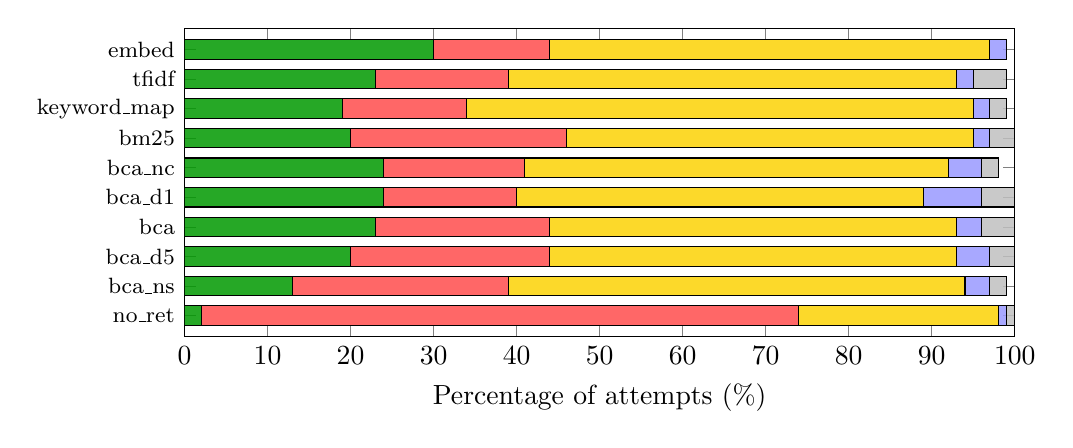
\begin{tikzpicture}
\begin{axis}[
    xbar stacked,
    width=\columnwidth,
    height=5.5cm,
    xlabel={Percentage of attempts (\%)},
    symbolic y coords={no\_ret, bca\_ns, bca\_d5, bca, bca\_d1, bca\_nc, bm25, keyword\_map, tfidf, embed},
    ytick=data,
    y tick label style={font=\footnotesize},
    xmin=0, xmax=100,
    legend to name=leg:failmodes,
    legend style={font=\scriptsize, legend columns=3, draw=none, column sep=4pt},
    area legend,
    bar width=7pt,
    enlarge y limits=0.08,
    every axis plot/.append style={fill opacity=0.85},
]
% Data: dev-report B=10k failure modes from Table 4 (exact values)
% pass
\addplot[fill=green!60!black] coordinates {(2,no\_ret) (13,bca\_ns) (20,bca\_d5) (23,bca) (24,bca\_d1) (24,bca\_nc) (20,bm25) (19,keyword\_map) (23,tfidf) (30,embed)};
% patch_apply_fail
\addplot[fill=red!70] coordinates {(72,no\_ret) (26,bca\_ns) (24,bca\_d5) (21,bca) (16,bca\_d1) (17,bca\_nc) (26,bm25) (15,keyword\_map) (16,tfidf) (14,embed)};
% test_fail
\addplot[fill=yellow!70!orange] coordinates {(24,no\_ret) (55,bca\_ns) (49,bca\_d5) (49,bca) (49,bca\_d1) (51,bca\_nc) (49,bm25) (61,keyword\_map) (54,tfidf) (53,embed)};
% syntax_error
\addplot[fill=blue!40] coordinates {(1,no\_ret) (3,bca\_ns) (4,bca\_d5) (3,bca) (7,bca\_d1) (4,bca\_nc) (2,bm25) (2,keyword\_map) (2,tfidf) (2,embed)};
% timeout
\addplot[fill=gray!50] coordinates {(1,no\_ret) (2,bca\_ns) (3,bca\_d5) (4,bca) (4,bca\_d1) (2,bca\_nc) (3,bm25) (2,keyword\_map) (4,tfidf) (0,embed)};
\legend{pass, patch\_fail, test\_fail, syntax, timeout}
\end{axis}
\end{tikzpicture}\\[4pt]
\ref{leg:failmodes}
\caption{Failure mode distribution at $\B{10\text{k}}$, dev-report. \textsc{no\_retrieval} is dominated by patch application failures (localization errors), while other methods shift toward test failures (comprehension errors).}
\label{fig:failure-modes}
\end{figure}

\subsection{Retrieval--Outcome Decoupling}\label{sec:decoupling}

Finding the right file does not guarantee a correct fix.  Appendix~\ref{app:supp-tables}
reports the full per-budget conversion tables for each tier
(\Cref{tab:conv-filehit-exact,tab:conv-filehit-devreport,tab:conv-filehit-vague}).
Here we focus on the cross-tier summary at $\B{10\text{k}}$ (\Cref{tab:conv-crosstier}).
\Cref{fig:conv-heatmap} visualizes this conversion collapse compactly.

\begin{table*}[tbp]
\centering
\caption{File hit $\to$ pass and symbol hit $\to$ pass conversion (\%) at $\B{10\text{k}}$, all tiers.}\label{tab:conv-crosstier}
\smallskip
\resizebox{\textwidth}{!}{%
\begin{tabular}{l cc cc cc}
\toprule
& \multicolumn{2}{c}{Dev-localized} & \multicolumn{2}{c}{Dev-report} & \multicolumn{2}{c}{Vague} \\
\cmidrule(lr){2-3}\cmidrule(lr){4-5}\cmidrule(lr){6-7}
Method & file$\to$pass & sym$\to$pass & file$\to$pass & sym$\to$pass & file$\to$pass & sym$\to$pass \\
\midrule
\textsc{bca}              & 72 & 72 & 24 & 24 &  3 &  3 \\
\textsc{bca\_d1}          & 79 & 76 & 25 & 25 &  3 &  3 \\
\textsc{bca\_d5}          & 73 & 69 & 21 & 21 &  2 &  2 \\
\textsc{bca\_no\_closure} & 76 & 76 & 25 & 26 &  2 &  3 \\
\textsc{bca\_no\_scoring} & 69 & 69 & 14 & 14 &  2 &  3 \\
\textsc{bm25}             & 79 & 81 & 22 & 23 & 12 & 11 \\
\textsc{keyword\_map}        & 77 & 76 & 19 & 22 &  3 &  5 \\
\textsc{tfidf}           & 86 & 84 & 23 & 26 &  8 &  7 \\
\textsc{embedding}       & 81 & 81 & 31 & 33 & 10 & 10 \\
\bottomrule
\end{tabular}%
}
\end{table*}

\begin{figure*}[tbp]
\centering
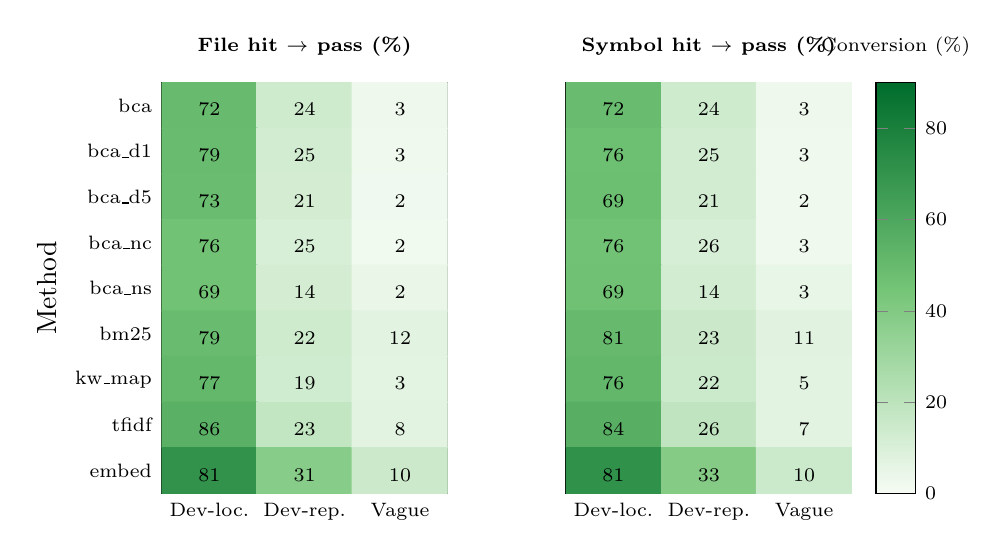
\begin{tikzpicture}
\begin{groupplot}[
  group style={group size=2 by 1, horizontal sep=1.5cm},
  width=0.43\textwidth,
  height=6.8cm,
  y dir=reverse,
  xmin=-0.5, xmax=2.5,
  ymin=-0.5, ymax=8.5,
  xtick={0,1,2},
  xticklabels={Dev-loc.,Dev-rep.,Vague},
  ytick={0,1,2,3,4,5,6,7,8},
  yticklabels={bca,bca\_d1,bca\_d5,bca\_nc,bca\_ns,bm25,kw\_map,tfidf,embed},
  point meta min=0,
  point meta max=90,
  colormap={hmconv}{rgb255=(247,252,245) rgb255=(116,196,118) rgb255=(0,109,44)},
  nodes near coords,
  every axis plot/.append style={draw=white, line width=0.45pt},
  every node near coord/.append style={
    font=\scriptsize,
    /pgf/number format/fixed,
    /pgf/number format/precision=0,
    text=black,
    anchor=center,
    yshift=-0.35ex
  },
  tick label style={font=\scriptsize},
  title style={font=\scriptsize\bfseries},
]
\nextgroupplot[title={File hit $\rightarrow$ pass (\%)}, ylabel={Method}]
\addplot[
  matrix plot*,
  shader=flat,
  mesh/cols=3,
  point meta=explicit,
] coordinates {
  (0,0) [72] (1,0) [24] (2,0) [3]
  (0,1) [79] (1,1) [25] (2,1) [3]
  (0,2) [73] (1,2) [21] (2,2) [2]
  (0,3) [76] (1,3) [25] (2,3) [2]
  (0,4) [69] (1,4) [14] (2,4) [2]
  (0,5) [79] (1,5) [22] (2,5) [12]
  (0,6) [77] (1,6) [19] (2,6) [3]
  (0,7) [86] (1,7) [23] (2,7) [8]
  (0,8) [81] (1,8) [31] (2,8) [10]
};

\nextgroupplot[title={Symbol hit $\rightarrow$ pass (\%)}, yticklabels={}, colorbar,
  colorbar style={
    title={Conversion (\%)},
    title style={font=\scriptsize},
    yticklabel style={font=\scriptsize},
    scaled y ticks=false,
    y dir=normal,
    every node near coord/.style={text opacity=0},
  }]
\addplot[
  matrix plot*,
  shader=flat,
  mesh/cols=3,
  point meta=explicit,
] coordinates {
  (0,0) [72] (1,0) [24] (2,0) [3]
  (0,1) [76] (1,1) [25] (2,1) [3]
  (0,2) [69] (1,2) [21] (2,2) [2]
  (0,3) [76] (1,3) [26] (2,3) [3]
  (0,4) [69] (1,4) [14] (2,4) [3]
  (0,5) [81] (1,5) [23] (2,5) [11]
  (0,6) [76] (1,6) [22] (2,6) [5]
  (0,7) [84] (1,7) [26] (2,7) [7]
  (0,8) [81] (1,8) [33] (2,8) [10]
};
\end{groupplot}
\end{tikzpicture}
\caption{Cross-tier retrieval-to-repair conversion at $\B{10\text{k}}$. Conversion is strong on dev-localized, collapses on dev-report, and is near-zero on vague, indicating a shift from retrieval bottlenecks to comprehension bottlenecks.}
\label{fig:conv-heatmap}
\end{figure*}

At $\B{10\text{k}}$, dev-localized is close to ``retrieval $\approx$ repair'':
69--86\% of attempts that include the target file also pass.  On dev-report,
that conversion drops to 14--25\%, and on vague it falls to 2--12\%.
Outside dev-localized, most correct retrievals still fail, indicating that
the bottleneck shifts from locating code to understanding and fixing it.

\paragraph{Passes without target file.}
This decoupling is further confirmed by the ``passes without target file''
metric (Appendix~\ref{app:supp-tables}, \Cref{tab:pass-without-file}).

On dev-localized, \textsc{no\_retrieval} produces 211 passes out
of 211, all without any context file, purely from the description.
On dev-report, only 0--1 passes occur without the target
file for retrieval methods.  On vague, 0--1 passes without the file.  The
LLM \emph{needs} code context for dev-report and vague queries; on
dev-localized queries, it does not.

\subsection{Hop Distance Analysis}\label{sec:hops}

We measure the graph distance (BFS hops on the undirected code knowledge
graph) from the nearest \emph{entity-mapped} seed symbol (derived from the
query text) to the mutation site.  This isolates the structural signal
available from explicit identifiers in the query and does not include BCA's
lexical fallbacks (e.g., BM25 seed boost or budget backfill).
Hop distributions by tier are reported in Appendix~\ref{app:supp-tables}
(\Cref{tab:hops}).  \Cref{tab:hops-pass1} and \Cref{fig:hops-pass1-heatmap}
show pass@1 as a function of hop distance on dev-report.

On dev-localized queries, entity extraction finds the exact mutated symbol
98\% of the time.  On dev-report, the traceback provides function names and
test names that resolve to symbols near the mutation (55\% direct hits,
36\% within 1--2~hops, and 9\% at 3--5~hops).  On vague queries, 89\% of
tasks have no reachable path from any extracted (entity-mapped) seed to the mutation.

\begin{table}[tbp]
\centering
\caption{Pass@1 by hop distance, BCA ($d$=3), dev-report.}\label{tab:hops-pass1}
\smallskip
\resizebox{\columnwidth}{!}{%
\begin{tabular}{lcccc r}
\toprule
Hop bucket & $\B{2\text{k}}$ & $\B{4\text{k}}$ & $\B{8\text{k}}$ & $\B{10\text{k}}$ & $N$ \\
\midrule
0 (direct)  & 0.15 & 0.19 & 0.27 & 0.35 & 135 \\
1--2 (near) & 0.06 & 0.04 & 0.04 & 0.07 &  89 \\
3--5 (mid)  & 0.05 & 0.19 & 0.14 & 0.19 &  21 \\
\bottomrule
\end{tabular}%
}
\end{table}

\begin{figure}[tbp]
\centering
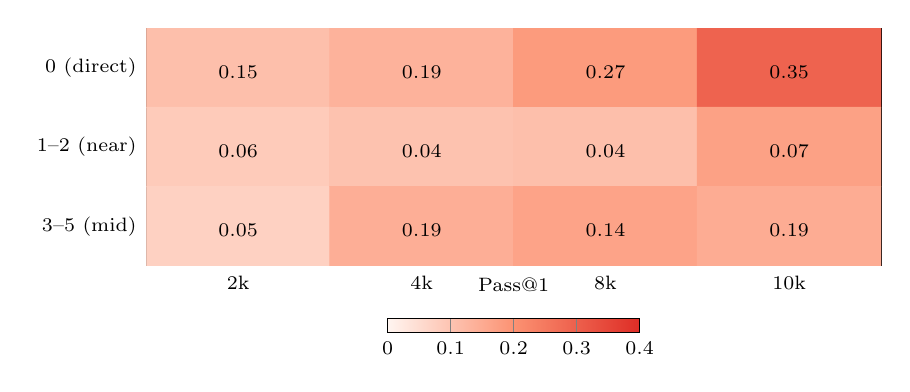
\begin{tikzpicture}
\begin{axis}[
  width=0.90\columnwidth,
  height=4.6cm,
  y dir=reverse,
  xmin=-0.5, xmax=3.5,
  ymin=-0.5, ymax=2.5,
  xtick={0,1,2,3},
  xticklabels={2k,4k,8k,10k},
  ytick={0,1,2},
  yticklabels={0 (direct),1--2 (near),3--5 (mid)},
  point meta min=0.00,
  point meta max=0.40,
  colormap={hmhops}{rgb255=(255,245,240) rgb255=(252,146,114) rgb255=(222,45,38)},
  colorbar horizontal,
  colorbar style={
    title={Pass@1},
    title style={font=\scriptsize},
    at={(0.5,-0.22)},
    anchor=north,
    width=3.2cm,
    height=1.8mm,
    xticklabel style={font=\scriptsize},
    scaled x ticks=false,
    every node near coord/.style={text opacity=0},
  },
  every axis plot/.append style={draw=white, line width=0.4pt},
  every node near coord/.append style={
    font=\scriptsize,
    /pgf/number format/fixed,
    /pgf/number format/precision=2,
    text=black,
    anchor=center,
    yshift=-0.35ex
  },
  nodes near coords,
  tick label style={font=\scriptsize},
]
\addplot[
  matrix plot*,
  shader=flat,
  mesh/cols=4,
  point meta=explicit,
] coordinates {
  (0,0) [0.15] (1,0) [0.19] (2,0) [0.27] (3,0) [0.35]
  (0,1) [0.06] (1,1) [0.04] (2,1) [0.04] (3,1) [0.07]
  (0,2) [0.05] (1,2) [0.19] (2,2) [0.14] (3,2) [0.19]
};
\end{axis}
\end{tikzpicture}
\caption{BCA dev-report pass@1 by hop bucket and budget. Darker cells indicate easier repair from structurally closer seeds.}
\label{fig:hops-pass1-heatmap}
\end{figure}

The 5$\times$ drop from hop-0~(0.35) to hop~1--2~(0.07) at $\B{10\text{k}}$
is a clear illustration that graph distance from seed to mutation predicts
repair difficulty.  Even one degree of structural indirection sharply
reduces the probability of a successful repair.

Appendix~\ref{app:supp-tables} extends this analysis across all methods at
$\B{10\text{k}}$ (\Cref{tab:hops-all-methods}).

At hop-0, BCA variants (0.35--0.36) slightly exceed TF-IDF~(0.32) and
bm25~(0.29).  At hop~1--2, \textsc{bca\_d1}~(0.12) and TF-IDF~(0.11) lead.
At 3+ hops ($N$=21, noisy), bm25 leads (0.24); for distant dependencies,
keyword matching may outperform graph traversal because the graph path is
too indirect.

Appendix~\ref{app:supp-tables} shows the corresponding analysis for
dev-localized queries, where 98\% of tasks are at hop-0 (\Cref{tab:hops-exact}).

\subsection{BCA Ablation}\label{sec:ablation}

\Cref{tab:ablation} reports the ablation of BCA's components, averaged
across all four budgets on dev-report.

\begin{table}[tbp]
\centering
\caption{BCA ablation on dev-report (average across budgets).}\label{tab:ablation}
\smallskip
\resizebox{\columnwidth}{!}{%
\begin{tabular}{lcc}
\toprule
Variant & Avg Pass@1 & $\Delta$ vs.\ BCA \\
\midrule
\textsc{bca\_no\_closure} & \textbf{0.18} & +2pp \\
\textsc{bca\_d1} ($d$=1) & \textbf{0.17} & +1pp \\
\textsc{bca} ($d$=3, full) & 0.16 & --- \\
\textsc{bca\_d5} ($d$=5)   & 0.15 & $-$1pp \\
\textsc{bca\_no\_scoring}  & 0.11 & $-$5pp \\
\bottomrule
\end{tabular}
}
\end{table}

\textbf{Scoring is BCA's essential component.}  Removing relevance scoring
drops performance by 5~percentage points, the largest effect in the
ablation.  Without scoring, BCA selects symbols by graph traversal order
alone, including many structurally connected but semantically irrelevant
symbols.

\textbf{Closure is negligible.}  Dependency closure consumes less than 1\%
of the budget for $d\geq3$ and its removal has no measurable effect on
pass@1.  Appendix~\ref{app:supp-tables} reports the detailed budget
consumption (\Cref{tab:closure}).

Closure overhead is tier-dependent.  \textsc{bca\_d1} uses 10\% on
dev-localized (many seeds produce many closure targets with a small frontier)
but only 1.7\% on dev-report.  For deeper expansions ($d\geq3$), closure
is negligible ($<$1\%) because the larger frontier already includes most
dependency paths.

\textbf{Shallower is slightly better.}  Depth~1 outperforms depth~3 by
1pp, and depth~3 outperforms depth~5 by 1pp.  Deeper expansion includes
more distant symbols that are less likely to be relevant.

\subsection{Retrieval Quality Metrics}\label{sec:retrieval-quality}

\Cref{tab:rq-devreport} reports retrieval quality metrics on dev-report (target
file and symbol hit rates), and \Cref{fig:rq-devreport-heatmap} provides a
matrix view.  The corresponding dev-localized and vague tables
are provided in Appendix~\ref{app:supp-tables} (\Cref{tab:rq-exact,tab:rq-vague}).

\begin{table*}[tbp]
\centering
\caption{Retrieval quality metrics, dev-report, all methods and budgets.}\label{tab:rq-devreport}
\smallskip
\resizebox{\textwidth}{!}{%
\begin{tabular}{l cccc cccc}
\toprule
& \multicolumn{4}{c}{Target file hit (\%)} & \multicolumn{4}{c}{Target symbol hit (\%)} \\
\cmidrule(lr){2-5}\cmidrule(lr){6-9}
Method & $\B{2\text{k}}$ & $\B{4\text{k}}$ & $\B{8\text{k}}$ & $\B{10\text{k}}$
       & $\B{2\text{k}}$ & $\B{4\text{k}}$ & $\B{8\text{k}}$ & $\B{10\text{k}}$ \\
\midrule
\textsc{bca}              & 89 & 92 & 96 & 96  & 72 & 80 & 86 & 90 \\
\textsc{bca\_d1}          & 89 & 91 & 96 & 96  & 72 & 82 & 90 & 94 \\
\textsc{bca\_d5}          & 89 & 91 & 96 & 96  & 71 & 80 & 86 & 90 \\
\textsc{bca\_no\_closure} & 89 & 92 & 96 & 96  & 72 & 80 & 87 & 91 \\
\textsc{bca\_no\_scoring} & 90 & 91 & 96 & 97  & 73 & 76 & 84 & 88 \\
\textsc{bm25}             & 80 & 84 & 89 & 89  & 73 & 78 & 82 & 83 \\
\textsc{no\_retrieval}    &  0 &  0 &  0 &  0  &  0 &  0 &  0 &  0 \\
\textsc{keyword\_map}        & 88 & 97 & 97 & 98  & 73 & 78 & 83 & 83 \\
\textsc{tfidf}           & 95 & 97 & 98 & 99  & 79 & 83 & 87 & 90 \\
\textsc{embedding}       & 91 & 95 & 98 & 98  & 78 & 81 & 86 & 85 \\
\bottomrule
\end{tabular}%
}
\end{table*}

\begin{figure*}[tbp]
\centering
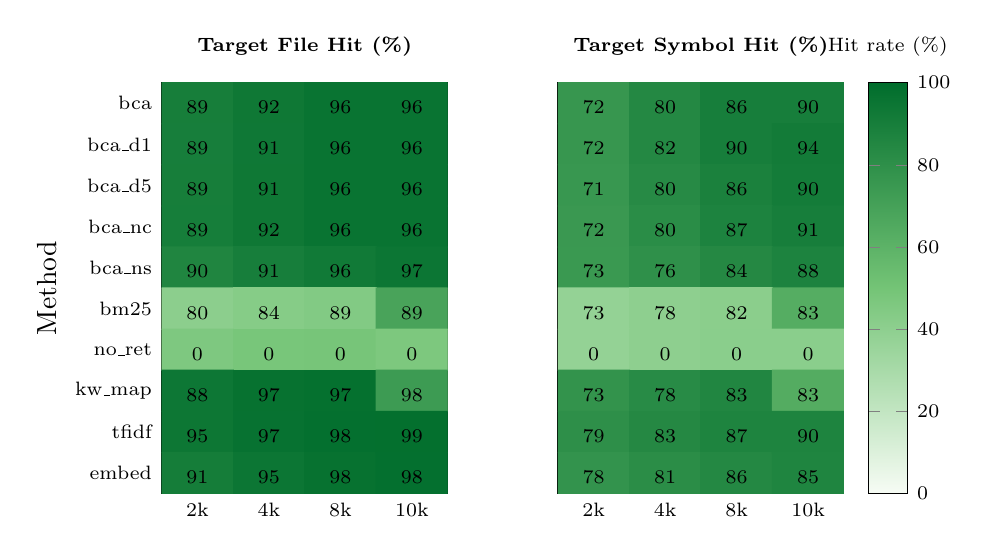
\begin{tikzpicture}
\begin{groupplot}[
  group style={group size=2 by 1, horizontal sep=1.4cm},
  width=0.43\textwidth,
  height=6.8cm,
  y dir=reverse,
  xmin=-0.5, xmax=3.5,
  ymin=-0.5, ymax=9.5,
  xtick={0,1,2,3},
  xticklabels={2k,4k,8k,10k},
  ytick={0,1,2,3,4,5,6,7,8,9},
  yticklabels={bca,bca\_d1,bca\_d5,bca\_nc,bca\_ns,bm25,no\_ret,kw\_map,tfidf,embed},
  point meta min=0,
  point meta max=100,
  colormap={hmrq}{rgb255=(247,252,245) rgb255=(116,196,118) rgb255=(0,109,44)},
  every axis plot/.append style={draw=white, line width=0.45pt},
  every node near coord/.append style={
    font=\scriptsize,
    /pgf/number format/fixed,
    /pgf/number format/precision=0,
    text=black,
    anchor=center,
    yshift=-0.35ex
  },
  nodes near coords,
  tick label style={font=\scriptsize},
  title style={font=\scriptsize\bfseries},
]
\nextgroupplot[title={Target File Hit (\%)}, ylabel={Method}]
\addplot[
  matrix plot*,
  shader=flat,
  mesh/cols=4,
  point meta=explicit,
] coordinates {
  (0,0) [89] (1,0) [92] (2,0) [96] (3,0) [96]
  (0,1) [89] (1,1) [91] (2,1) [96] (3,1) [96]
  (0,2) [89] (1,2) [91] (2,2) [96] (3,2) [96]
  (0,3) [89] (1,3) [92] (2,3) [96] (3,3) [96]
  (0,4) [90] (1,4) [91] (2,4) [96] (3,4) [97]
  (0,5) [80] (1,5) [84] (2,5) [89] (3,5) [89]
  (0,6) [0]  (1,6) [0]  (2,6) [0]  (3,6) [0]
  (0,7) [88] (1,7) [97] (2,7) [97] (3,7) [98]
  (0,8) [95] (1,8) [97] (2,8) [98] (3,8) [99]
  (0,9) [91] (1,9) [95] (2,9) [98] (3,9) [98]
};

\nextgroupplot[
  title={Target Symbol Hit (\%)},
  yticklabels={},
  colorbar,
  colorbar style={
    title={Hit rate (\%)},
    title style={font=\scriptsize},
    yticklabel style={font=\scriptsize},
    scaled y ticks=false,
    y dir=normal,
    every node near coord/.style={text opacity=0},
  }
]
\addplot[
  matrix plot*,
  shader=flat,
  mesh/cols=4,
  point meta=explicit,
] coordinates {
  (0,0) [72] (1,0) [80] (2,0) [86] (3,0) [90]
  (0,1) [72] (1,1) [82] (2,1) [90] (3,1) [94]
  (0,2) [71] (1,2) [80] (2,2) [86] (3,2) [90]
  (0,3) [72] (1,3) [80] (2,3) [87] (3,3) [91]
  (0,4) [73] (1,4) [76] (2,4) [84] (3,4) [88]
  (0,5) [73] (1,5) [78] (2,5) [82] (3,5) [83]
  (0,6) [0]  (1,6) [0]  (2,6) [0]  (3,6) [0]
  (0,7) [73] (1,7) [78] (2,7) [83] (3,7) [83]
  (0,8) [79] (1,8) [83] (2,8) [87] (3,8) [90]
  (0,9) [78] (1,9) [81] (2,9) [86] (3,9) [85]
};
\end{groupplot}
\end{tikzpicture}
\caption{Dev-report retrieval quality heatmaps. File hit saturates for most methods by 8k--10k, while symbol hit remains more discriminative.}
\label{fig:rq-devreport-heatmap}
\end{figure*}

Tracebacks improve file retrieval: TF-IDF jumps from 75--84\%
(dev-localized) to 95--99\% (dev-report) because traceback text
contains function names that TF-IDF matching finds.
\textsc{keyword\_map} maintains 88--98\% on dev-report and achieves
uniquely high vague-tier retrieval (56--96\%) because it includes a
repository-wide file tree (all paths).  On vague queries,
\textsc{bca\_d5} and \textsc{bca\_no\_closure} show the strongest
file hit growth with budget (31$\to$71\% and 28$\to$73\%), as deeper
graph expansion eventually reaches the target.

\textsc{bca\_d1} achieves the highest symbol hit rate on dev-report
at $\B{10\text{k}}$ (94\%): traceback-derived seeds resolve into precise
graph symbols, and shallow expansion focuses on the immediate neighborhood.
On vague queries, \textsc{bca\_d5} achieves 53\% symbol hit at
$\B{10\text{k}}$, the highest among all methods, while keyword and TF-IDF
methods plateau at 40\%.

\subsection{Edit Locality and Patch Quality}\label{sec:edit-locality}

\paragraph{Edit distance.}
Appendix~\ref{app:supp-tables} reports the full edit distance tables across
tiers and budgets (\Cref{tab:editdist-devreport,tab:editdist-exact,tab:editdist-vague}).

Edit distance follows the three-tier gradient.  On dev-localized,
\textsc{no\_retrieval} achieves a mean distance of 0.5~lines (the
description says exactly where to edit).  On dev-report, distances range
from 44~lines (\textsc{keyword\_map}) to 143~lines (\textsc{no\_retrieval}).
On vague, distances range from 28 to 209~lines, with BCA variants and
\textsc{keyword\_map} showing the highest distances because they include
structurally related but distant code.

\paragraph{Context--patch overlap.}
The fraction of context files referenced in the generated patch reveals the
degree to which the LLM uses the provided context.
Appendix~\ref{app:supp-tables} reports the full overlap tables
(\Cref{tab:overlap-devreport,tab:overlap-exact,tab:overlap-vague}).

BCA methods produce the highest context--patch overlap on dev-report
(0.15--0.42): the LLM references BCA-provided context files more often in
its patches than it references context from other methods.  On vague queries,
\textsc{keyword\_map} achieves the highest overlap (0.18--0.33) because its
signature-dense context covers more of the codebase.  All overlap values
generally decrease with budget as the context grows larger relative to
the patch.  \textsc{bm25} and \textsc{tfidf} have consistently low overlap
(0.04--0.16), indicating their contexts include many files the LLM ignores.

\paragraph{Patch size.}
Appendix~\ref{app:supp-tables} reports patch size statistics for all attempts
and passing attempts (\Cref{tab:patchsize}).

Passing patches change 1.2--2.6~lines on average, while all-attempt averages
are 1.9--6.4~lines. Over-editing (making more changes than necessary) correlates with failure. This holds across all tiers and methods.

\subsection{Per-Repository Analysis}\label{sec:per-repo}

The two repositories exhibit different method rankings across all three
tiers.  Appendix~\ref{app:supp-tables} provides the full budget sweep per
repository (\Cref{tab:httpx-devreport,tab:pydantic-devreport,tab:httpx-exact,tab:pydantic-exact,tab:httpx-vague,tab:pydantic-vague}).

Method rankings flip between repositories.  On httpx dev-report,
embedding leads at $\B{10\text{k}}$ (0.34) while TF-IDF
leads at lower budgets (0.27--0.30), and on pydantic-ai, BCA variants
overtake at $\B{10\text{k}}$ (0.25--0.27 vs.\ TF-IDF's 0.20).  The larger,
more complex pydantic-ai codebase gives BCA's graph traversal more
structural signal to exploit.  On dev-localized, \textsc{no\_retrieval}
leads both repositories (httpx: 0.91, pydantic-ai: 0.81).  On vague,
most methods are near-zero on httpx ($\leq$0.05), though embedding reaches
0.11--0.13; pydantic-ai shows slightly better discrimination with bm25
achieving 0.07--0.09.  Different codebases reward different retrieval
strategies.

\subsection{Decomposition by Mutation Type}\label{sec:decomposition}

Performance varies substantially by mutation type on dev-report.
Appendix~\ref{app:supp-tables} provides full tables for all methods at
$\B{2\text{k}}$ and $\B{10\text{k}}$ (\Cref{tab:muttype-2k,tab:muttype-10k}).

\texttt{none\_check\_swap} remains the hardest mutation type (58~tasks, best
method only 16\% at $\B{10\text{k}}$).  These mutations flip
\texttt{if x is None} to \texttt{if x is not None}, semantically subtle
changes difficult to diagnose from a traceback alone.
\texttt{constant\_mutation} and \texttt{handcrafted} are the easiest (up to
50\%), as the changed values are often visible in test output.  At
$\B{2\text{k}}$, BCA variants underperform keyword and TF-IDF methods on
most mutation types; at $\B{10\text{k}}$, BCA closes the gap and leads on
\texttt{constant\_mutation} (\textsc{bca\_nc}:~0.50) and
\texttt{handcrafted} (\textsc{bca\_nc}:~0.50).

\subsection{Conditional Bins}\label{sec:bins}

We decompose pass@1 by three conditioning variables: identifier density
(fraction of query tokens that are code identifiers), hop distance from the
nearest BCA seed to the mutation site, and mutation size (lines in the
mutated function).  We show all three tiers at $\B{2\text{k}}$ and
$\B{10\text{k}}$.

\paragraph{Identifier density.}
Appendix~\ref{app:supp-tables} reports pass@1 binned by whether the query
contains code identifiers (\Cref{tab:bin-ident-exact,tab:bin-ident-devreport,tab:bin-ident-vague}).

On dev-localized, the zero-identifier queries ($N$=95, where the description
uses natural language rather than code tokens) actually favor
\textsc{no\_retrieval} more strongly (0.95 vs.\ 0.81), consistent with the
model leveraging location information from the prose description.  On
dev-report, all 245 queries have identifiers (traceback tokens are always
present).  On vague, only 4~queries contain identifiers; these show
dramatically higher pass rates (e.g., bm25: 0.50 vs.\ 0.06) but the sample
is too small for robust conclusions.

\paragraph{Hop distance.}
\Cref{tab:bin-hops-2k,tab:bin-hops-10k,tab:bin-hops-exact,tab:bin-hops-vague}
are provided in Appendix~\ref{app:supp-tables}.

At hop-0, BCA variants improve dramatically from $\B{2\text{k}}$ to
$\B{10\text{k}}$ (e.g., \textsc{bca\_nc}: 0.15$\to$0.36), nearly matching
TF-IDF (0.30$\to$0.32).  At hop~1--2, all methods remain low (0.04--0.12),
confirming that even one degree of structural indirection sharply reduces
repair probability regardless of method or budget.  At 3+ hops ($N$=21),
bm25 leads at $\B{10\text{k}}$ (0.24); for distant dependencies, keyword
matching outperforms graph traversal.

On dev-localized, 240/245 tasks are hop-0 (the description directly names
the mutated symbol), so the hop distribution is degenerate.  On vague
queries, 89\% of tasks (219/245) are unreachable from any seed; entity
extraction from symptom-only text yields almost no graph-resolvable
identifiers.  The few reachable vague tasks (1--2 hops, $N$=16) show the
only nonzero pass rates, with bm25 at 0.12 and BCA variants at 0.06.

\paragraph{Mutation size.}
\Cref{tab:bin-size-2k,tab:bin-size-10k,tab:bin-size-exact,tab:bin-size-vague}
are provided in Appendix~\ref{app:supp-tables}.

At $\B{2\text{k}}$, BCA variants score 0.00 on the smallest mutations
($<$5~lines, $N$=10), while TF-IDF achieves 0.30. These are highly
localized changes where keyword similarity suffices.  At $\B{10\text{k}}$,
BCA catches up (0.20--0.30).  For medium mutations (20--49~lines),
\textsc{bca\_d1} leads at $\B{10\text{k}}$ (0.31), slightly ahead of
\textsc{bca\_nc} (0.28) and TF-IDF (0.26).  The 100+ line bin ($N$=8) is
too small for reliable conclusions, but TF-IDF maintains 0.25 across both
budgets.

On dev-localized, \textsc{no\_retrieval} achieves 1.00 on 100+ line
functions: these are large, well-documented functions where the file+line
description is fully sufficient.  BCA variants struggle on 50--99 line
functions at $\B{2\text{k}}$ (0.25--0.47) but improve substantially at
$\B{10\text{k}}$ (0.43--0.66).  On vague queries, only small functions
($<$5~lines) show any meaningful signal; all methods score $\leq$0.30,
and 50+ line functions are effectively unsolvable from vague descriptions.
Overall, no method dominates across all size bins, reinforcing the case for
conditional routing.

\subsection{Context Efficiency}\label{sec:efficiency}

\Cref{tab:efficiency} is provided in Appendix~\ref{app:supp-tables}.

Higher symbol density does not correlate with higher pass@1.
\textsc{bca\_d5} packs the most symbols (15.3/1k on dev-localized) but does
not outperform \textsc{bm25} (9.4/1k).  \textsc{keyword\_map} has the lowest
density (1.2--2.0) but strong performance because function signatures are
information-dense.  The quality of selected symbols matters more than
the quantity.

% ══════════════════════════════════════════════════════════════════════════════

\section{Conditional Routing}\label{sec:routing}

A natural question following the method-comparison results is whether a lightweight classifier can select the best retrieval method per task, rather than committing to a single method globally.
We train two logistic-regression routers and evaluate them under leave-one-out cross-validation (LOO-CV) on the solvable subset of each budget slice.

\subsection{Router Design}\label{sec:router-design}

\begin{figure*}[tbp]
\centering
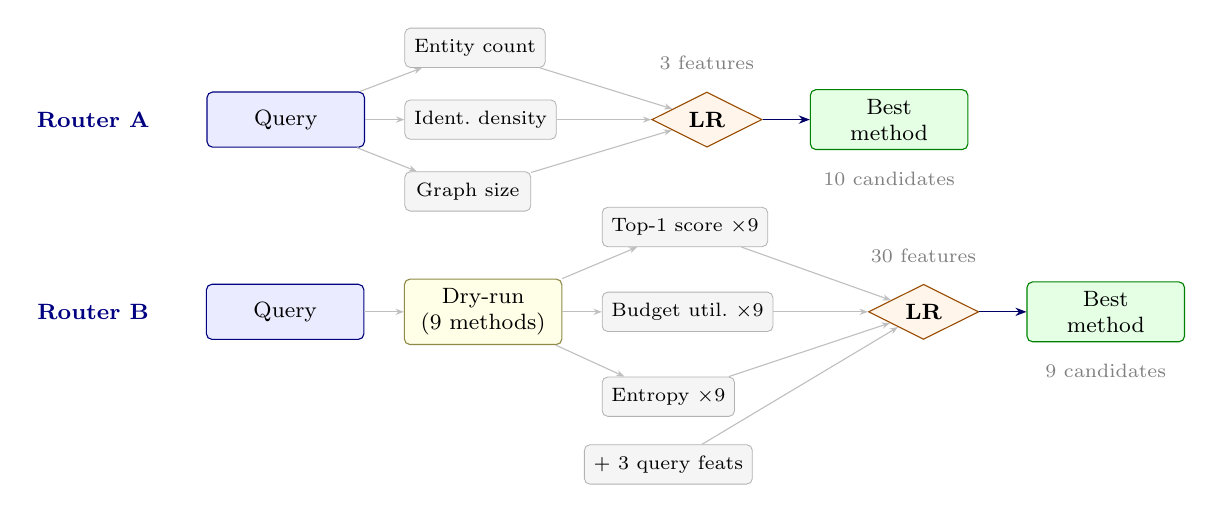
\begin{tikzpicture}[
  box/.style={rectangle, rounded corners=2pt, draw=blue!50!black, fill=blue!8,
    minimum width=2cm, minimum height=0.7cm, font=\footnotesize, align=center,
    line width=0.4pt},
  feat/.style={rectangle, rounded corners=2pt, draw=gray!60, fill=gray!8,
    minimum width=1.6cm, minimum height=0.5cm, font=\scriptsize, align=center,
    line width=0.3pt},
  decision/.style={diamond, draw=orange!60!black, fill=orange!8,
    minimum width=1.4cm, minimum height=0.7cm, font=\footnotesize\bfseries,
    align=center, inner sep=1pt, aspect=2, line width=0.4pt},
  arrow/.style={-{Stealth[length=4pt]}, blue!40!black},
  garrow/.style={-{Stealth[length=3pt]}, gray!50},
  node distance=0.4cm and 0.5cm
]

% Router A path (top)
\node[font=\footnotesize\bfseries, text=blue!50!black] (ra_label) {Router A};
\node[box, right=0.6cm of ra_label] (query) {Query};

\node[feat, above right=0.3cm and 0.5cm of query] (f1) {Entity count};
\node[feat, right=0.5cm of query] (f2) {Ident.\ density};
\node[feat, below right=0.3cm and 0.5cm of query] (f3) {Graph size};

\draw[garrow] (query) -- (f1);
\draw[garrow] (query) -- (f2);
\draw[garrow] (query) -- (f3);

\node[decision, right=1.2cm of f2] (lr_a) {LR};
\node[box, right=0.6cm of lr_a, fill=green!10, draw=green!50!black] (method_a) {Best\\method};

\draw[garrow] (f1) -- (lr_a);
\draw[garrow] (f2) -- (lr_a);
\draw[garrow] (f3) -- (lr_a);
\draw[arrow] (lr_a) -- (method_a);

\node[font=\scriptsize, text=black!50, above=0.15cm of lr_a] {3 features};
\node[font=\scriptsize, text=black!50, below=0.15cm of method_a] {10 candidates};

% Router B path (bottom)
\node[font=\footnotesize\bfseries, text=blue!50!black, below=2.0cm of ra_label] (rb_label) {Router B};
\node[box, right=0.6cm of rb_label] (query_b) {Query};

\node[box, right=0.5cm of query_b, fill=yellow!10, draw=yellow!50!black] (dryrun) {Dry-run\\(9 methods)};

\node[feat, above right=0.4cm and 0.5cm of dryrun] (df1) {Top-1 score $\times$9};
\node[feat, right=0.5cm of dryrun] (df2) {Budget util.\ $\times$9};
\node[feat, below right=0.4cm and 0.5cm of dryrun] (df3) {Entropy $\times$9};

\draw[garrow] (query_b) -- (dryrun);
\draw[garrow] (dryrun) -- (df1);
\draw[garrow] (dryrun) -- (df2);
\draw[garrow] (dryrun) -- (df3);

\node[decision, right=1.2cm of df2] (lr_b) {LR};
\node[box, right=0.6cm of lr_b, fill=green!10, draw=green!50!black] (method_b) {Best\\method};

\draw[garrow] (df1) -- (lr_b);
\draw[garrow] (df2) -- (lr_b);
\draw[garrow] (df3) -- (lr_b);

% Also feed the 3 query features into Router B
\node[feat, below=0.35cm of df3] (qf) {+ 3 query feats};
\draw[garrow] (qf) -- (lr_b);

\draw[arrow] (lr_b) -- (method_b);

\node[font=\scriptsize, text=black!50, above=0.15cm of lr_b] {30 features};
\node[font=\scriptsize, text=black!50, below=0.15cm of method_b] {9 candidates};

\end{tikzpicture}
\caption{Router architectures. Router~A uses only pre-retrieval query features. Router~B adds dry-run retrieval confidence statistics (no extra LLM calls), adding $\sim$1\,s of additional local assembly time in our setup (Appendix~\ref{app:cost-latency}).}
\label{fig:router-arch}
\end{figure*}

\paragraph{Router~A (pre-retrieval).}
Uses three query-level features available before any retrieval:
the number of query entities that resolve to graph nodes,
the fraction of query tokens that are code identifiers,
and the log-transformed graph size.
Candidate set: all ten methods.  Zero latency overhead.

\paragraph{Router~B (dry-run).}
Extends Router~A with 27 retrieval-signal features: for each of nine
retrieval methods, a single cheap dry-run produces three
statistics (top-1 retrieval score, budget utilisation fraction, and
softmax entropy over retrieved items), yielding $3 + 9 \times 3 = 30$
features total.  The candidate set contains nine methods (excluding
\textsc{no\_retrieval}, since the dry-run signals are undefined for it).
Dry-running all nine methods adds $\sim$1\,s of additional assembly time
while avoiding extra LLM calls (Appendix~\ref{app:cost-latency}).
In router-feature tables, prefixes follow the method identifiers in our
artifacts; e.g., \texttt{vector\_*} corresponds to the TF-IDF method
(\textsc{tfidf} in this paper).

\paragraph{Label strategies.}
We consider two strategies for assigning the training label when multiple methods solve a task:
\begin{itemize}[nosep]
  \item \emph{Smart}: label = best single method if it passes, else the rarest passer (encouraging selective deviations).
  \item \emph{Safest}: always assign the most-frequently-passing method (maximizing label stability).
\end{itemize}

Both routers use $\ell_2$-regularized logistic regression with LOO-CV on the solvable tasks at each budget.

\subsection{Router Results}\label{sec:router-results}

Table~\ref{tab:router-devreport} reports router performance on the dev-report tier.
Full router tables for dev-localized and vague are provided in Appendix~\ref{app:routing-details}
(Tables~\ref{tab:router-localized} and~\ref{tab:router-vague}).
Because Router~A and Router~B use different candidate sets, their baselines
(majority vote and random) and solvable-task pools can differ; we report
them separately.  Parenthesized deltas are percent of the oracle gap closed,
computed per router as $\frac{\text{Router} - \text{Maj}}{\text{Oracle} - \text{Maj}} \times 100$.

\begin{table*}[tbp]
\centering
\caption{Router comparison on \textbf{dev-report} tasks (LOO-CV). Baselines and $N$ are reported per router because candidate sets differ.}
\label{tab:router-devreport}
\resizebox{\textwidth}{!}{%
\begin{tabular}{l r r r r r r r r r r}
\toprule
& \multicolumn{5}{c}{Router~A (10 candidates)} & \multicolumn{5}{c}{Router~B (9 candidates)} \\
\cmidrule(lr){2-6} \cmidrule(lr){7-11}
Budget & Maj(A) & Rnd(A) & Smart & Safest & $N$(A) & Maj(B) & Rnd(B) & Smart & Safest & $N$(B) \\
\midrule
\B{2\text{k}}  & 57.1\% & 33.5\% & 59.2\% \small{(+4.8\%)} & 59.2\% \small{(+4.8\%)} & 98  & 57.7\% & 36.9\% & 69.1\% \small{(+26.8\%)} & 69.1\% \small{(+26.8\%)} & 97 \\
\B{4\text{k}}  & 55.2\% & 35.3\% & 59.0\% \small{(+8.5\%)}  & 55.2\% \small{(+0.0\%)}  & 105 & 55.2\% & 38.6\% & 58.1\% \small{(+6.4\%)}  & 56.2\% \small{(+2.1\%)}  & 105 \\
\B{8\text{k}}  & 54.7\% & 38.1\% & 53.8\% \small{(-1.9\%)} & 56.4\% \small{(+3.8\%)}  & 117 & 54.7\% & 41.8\% & 64.1\% \small{(+20.8\%)} & 62.4\% \small{(+17.0\%)} & 117 \\
\B{10\text{k}} & 62.2\% & 41.3\% & 66.4\% \small{(+11.1\%)} & 65.5\% \small{(+8.9\%)} & 119 & 62.2\% & 45.3\% & 62.2\% \small{(+0.0\%)} & 61.3\% \small{(-2.2\%)} & 119 \\
\bottomrule
\end{tabular}%
}
\end{table*}

\paragraph{Summary.}
On dev-report tasks, Router~B with the \emph{smart} label strategy achieves the largest single gain (+26.8\% relative at \B{2\text{k}}), while the \emph{safest} strategy is more consistently positive across budgets.
On dev-localized tasks, the majority-vote baseline already captures 78--89\% of tasks, leaving little room for routing improvements; both routers match or marginally improve upon the baseline.
On vague tasks ($N = 28\text{--}34$), the routers frequently underperform majority vote, confirming that the small sample size precludes reliable per-instance discrimination.

\paragraph{End-to-end pass@1 after routing.}
The LOO-CV numbers above evaluate routing on the \emph{solvable} subset (tasks with at least one passing method under the candidate set).  To report an end-to-end view, we also compute dev-report pass@1 over all 245 tasks by selecting the router-chosen method's \emph{existing} single-shot attempt for each task (no additional LLM calls).
Table~\ref{tab:routed-pass1} shows that routing yields modest pass@1 gains over the best fixed method at most budgets, though Router~B merely matches the best fixed method at $\B{10\text{k}}$.

\paragraph{Statistical significance.}
To assess whether these gains are reliable, we run paired bootstrap tests (10,000 resamples) comparing Router~B (smart) pass@1 against the best fixed method (embedding) on a per-task basis for dev-report:
$\B{2\text{k}}$: $+$4.5pp, 95\% CI [$+$1.2, $+$8.2], $p \approx 0.01$;
$\B{4\text{k}}$: $+$1.2pp, 95\% CI [$-$1.2, $+$3.7], $p \approx 0.40$;
$\B{8\text{k}}$: $+$4.5pp, 95\% CI [$+$1.6, $+$7.8], $p < 0.01$;
$\B{10\text{k}}$: $+$0.0pp, 95\% CI [$-$2.4, $+$2.4], $p \approx 1.00$.
The gains at $\B{2\text{k}}$ and $\B{8\text{k}}$ are statistically significant at $\alpha = 0.05$, while $\B{4\text{k}}$ and $\B{10\text{k}}$ are not.
We therefore frame routing as a \emph{partial validation} of the conditional assembly thesis: the oracle gap is real (17--22pp), method complementarity exists (25--32\% sole-solvers), and a lightweight router can close part of the gap at some budgets.
Scaling to more tasks or using a richer model class may yield significance across all budgets.

\begin{table}[tbp]
\centering
\caption{Dev-report end-to-end pass@1 after routing (245 tasks). ``Best fixed'' is the best single method from Table~\ref{tab:devreport}; routers select among their candidate sets via LOO-CV.}
\label{tab:routed-pass1}
\smallskip
\resizebox{\columnwidth}{!}{%
\begin{tabular}{lcccc}
\toprule
Budget & Best fixed & Router~A (safest) & Router~B (smart) & Oracle \\
\midrule
\B{2\text{k}}  & 0.229 (\textsc{embedding}) & 0.237 & 0.273 & 0.400 \\
\B{4\text{k}}  & 0.237 (\textsc{embedding}) & 0.237 & 0.249 & 0.429 \\
\B{8\text{k}}  & 0.261 (\textsc{embedding}) & 0.269 & 0.306 & 0.478 \\
\B{10\text{k}} & 0.302 (\textsc{embedding}) & 0.322 & 0.302 & 0.486 \\
\bottomrule
\end{tabular}%
}
\end{table}

\paragraph{Post-hoc analysis.}
Independently of the deployment routers above, we fit a post-hoc logistic regression router using 7~features (3~query-level plus 4~retrieval-confidence metrics) for interpretability.
Results are reported in Appendix~\ref{app:routing-details} (Table~\ref{tab:posthoc-router}).

% ── Chart: Router gap comparison on dev-report ───────────────────────────────
\begin{figure}[tbp]
\centering
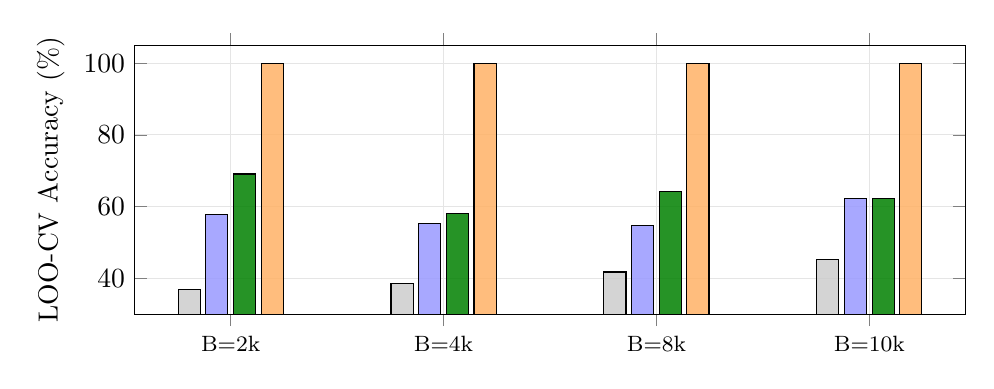
\begin{tikzpicture}
\begin{axis}[
    ybar,
    bar width=8pt,
    width=\columnwidth,
    height=5cm,
    ylabel={LOO-CV Accuracy (\%)},
    symbolic x coords={B=2k, B=4k, B=8k, B=10k},
    xtick=data,
    ymin=30, ymax=105,
    legend to name=leg:routergap,
    legend style={font=\scriptsize, legend columns=4, draw=none},
    enlarge x limits=0.15,
    grid=major,
    grid style={gray!20},
    every axis plot/.append style={fill opacity=0.85},
    x tick label style={font=\footnotesize},
]
% Router data: dev-report
% Random
\addplot[fill=gray!40] coordinates {(B=2k,36.9) (B=4k,38.6) (B=8k,41.8) (B=10k,45.3)};
% Majority
\addplot[fill=blue!40] coordinates {(B=2k,57.7) (B=4k,55.2) (B=8k,54.7) (B=10k,62.2)};
% Router B (smart) -- best performing
\addplot[fill=green!50!black] coordinates {(B=2k,69.1) (B=4k,58.1) (B=8k,64.1) (B=10k,62.2)};
% Oracle
\addplot[fill=orange!60] coordinates {(B=2k,100) (B=4k,100) (B=8k,100) (B=10k,100)};
\legend{Random, Majority, Router B, Oracle}
\end{axis}
\end{tikzpicture}\\[4pt]
\ref{leg:routergap}
\caption{Router B (smart) vs.\ baselines on dev-report (LOO-CV). The gap between Majority and Oracle represents the routing opportunity. Router B closes 26.8\% of this gap at $\B{2\text{k}}$.}
\label{fig:router-gap}
\end{figure}

\subsection{Why Dev-Report Enables Routing}\label{sec:sole-solvers}

The router's opportunity is bounded by method complementarity: if a single method solves every task, no routing can help.
We quantify complementarity via \emph{sole-solver} analysis, tasks solved by exactly one method.

\begin{table*}[tbp]
\centering
\caption{Sole-solver analysis across tiers. ``Multi'' = solved by $\geq 2$ methods; ``Sole'' = solved by exactly one.}
\label{tab:sole-solvers}
\resizebox{\textwidth}{!}{%
\begin{tabular}{l r r r r l}
\toprule
Tier / Budget & Solvable & Multi & Sole & Sole \% & Top Sole-Solver Methods \\
\midrule
\multicolumn{6}{l}{\textit{Dev-report}} \\
\B{2\text{k}}  & 98  & 67 & 31 & 31.6\% & \textsc{embedding}(12), \textsc{tfidf}(7), \textsc{keyword\_map}(5), \textsc{bm25}(4), \textsc{bca}(2), \textsc{no\_retrieval}(1) \\
\B{4\text{k}}  & 105 & 74 & 31 & 29.5\% & \textsc{embedding}(9), \textsc{bm25}(7), \textsc{keyword\_map}(6), \textsc{tfidf}(4), \textsc{bca}(1), \textsc{bca\_d1}(1), others(3) \\
\B{8\text{k}}  & 117 & 84 & 33 & 28.2\% & \textsc{embedding}(11), \textsc{keyword\_map}(7), \textsc{bm25}(4), \textsc{tfidf}(4), \textsc{bca\_no\_scoring}(3), \textsc{bca\_d1}(2), others(2) \\
\B{10\text{k}} & 119 & 89 & 30 & 25.2\% & \textsc{embedding}(17), \textsc{bm25}(3), \textsc{keyword\_map}(3), \textsc{bca\_d1}(2), \textsc{bca\_no\_closure}(2), \textsc{tfidf}(2), \textsc{bca\_no\_scoring}(1) \\
\midrule
\multicolumn{6}{l}{\textit{Dev-localized}} \\
\B{2\text{k}}  & 238 & 232 & 6  & 2.5\% & \textsc{no\_retrieval}(4), \textsc{tfidf}(2) \\
\B{4\text{k}}  & 239 & 232 & 7  & 2.9\% & \textsc{no\_retrieval}(5), \textsc{tfidf}(2) \\
\B{8\text{k}}  & 238 & 235 & 3  & 1.3\% & \textsc{no\_retrieval}(3) \\
\B{10\text{k}} & 240 & 237 & 3  & 1.3\% & \textsc{no\_retrieval}(2), \textsc{embedding}(1) \\
\midrule
\multicolumn{6}{l}{\textit{Vague}} \\
\B{2\text{k}}  & 34 & 15 & 19 & 55.9\% & \textsc{embedding}(14), \textsc{bm25}(4), \textsc{keyword\_map}(1) \\
\B{4\text{k}}  & 30 & 15 & 15 & 50.0\% & \textsc{embedding}(13), \textsc{bm25}(1), \textsc{bca\_d1}(1) \\
\B{8\text{k}}  & 30 & 13 & 17 & 56.7\% & \textsc{embedding}(14), \textsc{bm25}(2), \textsc{bca\_d1}(1) \\
\B{10\text{k}} & 28 & 11 & 17 & 60.7\% & \textsc{embedding}(13), \textsc{bm25}(4) \\
\bottomrule
\end{tabular}%
}
\end{table*}

Dev-report tasks exhibit 25--32\% sole-solvers, spread across six or more methods (with \textsc{embedding} contributing the most unique solves at every budget), sufficient diversity for a router to exploit.
Dev-localized tasks show only 1--3\% sole-solvers, almost all attributable to \textsc{no\_retrieval}, explaining why routers match but cannot beat the majority baseline.
Vague tasks have the highest sole-solver fraction (up to 61\%), dominated by \textsc{embedding} (13--14 sole solves per budget), but the absolute solvable counts ($N \leq 34$) are too small for LOO-CV to learn stable decision boundaries.

\paragraph{Feature signals.}
Router~B's strongest coefficients are retrieval-confidence features such as entropy and top-1 score, while Router~A relies
primarily on identifier density and mapped-entity count.
Full coefficient tables are provided in Appendix~\ref{app:routing-details}
(Tables~\ref{tab:feature-importance} and~\ref{tab:feature-importance-a}).


% ══════════════════════════════════════════════════════════════════════════════
\section{Discussion}\label{sec:discussion}

\paragraph{Context assembly is conditional.}
The central result of this study is that context assembly is not a universal
retrieval problem.  It is conditional on query information content.  When
the query leaks the bug location (dev-localized), retrieval is unnecessary
and can reduce performance.  When the query provides structural clues like
tracebacks (dev-report), retrieval quality matters and method choice matters.
When the query is purely symptomatic (vague), model comprehension is the
bottleneck, and differences between retrieval methods are small relative to
the overall low pass rates.

This has practical implications.  Real developer queries span this spectrum.
A system that routes queries to the appropriate retrieval strategy, or
bypasses retrieval entirely when the query is self-sufficient, can
outperform a single fixed retrieval method, especially on dev-report tasks.
Our router results provide initial
evidence for this claim, closing up to 26.8\% of the oracle gap on the
dev-report tier with zero additional LLM calls.

\paragraph{Graph-guided retrieval: regime-dependent.}
The BCA ablation reveals when graph-guided retrieval helps and why:

\begin{itemize}[leftmargin=*,nosep]
  \item On dev-report at higher budgets, BCA variants narrow the gap with
    TF-IDF; at $\B{10\text{k}}$ the best BCA variants match or slightly
    exceed TF-IDF.
  \item On dev-report at low budget, BCA underperforms because it cannot fit
    both seeds and their neighborhoods into the tight context window.
  \item On dev-localized, BCA underperforms because entity extraction from
    file-and-line descriptions produces less precise seeds than on
    tracebacks.
  \item On vague queries, BCA is no better than other methods: the graph
    component is often starved of entity-mapped seeds (89\% unreachable), and
    the lexical fallbacks/backfill do not materially change pass@1.
\end{itemize}

The ablation shows that relevance scoring is BCA's critical component
($-$5pp when removed), not expansion depth or closure.  Future work should
focus on improving scoring functions rather than expanding graph traversal.

\paragraph{Context--patch overlap.}
BCA produces higher context--patch overlap than TF-IDF on dev-report
(0.17--0.19 vs.\ 0.04--0.07), meaning the LLM references BCA-provided context
files more frequently in its generated patches.  However, higher overlap
does not translate to higher pass@1; \textsc{embedding} leads overall.  This
metric is descriptive, not prescriptive: it shows that BCA's graph-guided
context is structurally closer to the edit site, but this proximity alone
is insufficient for repair.

\paragraph{Routing headroom.}
On dev-report, the oracle pass@1 is 0.40--0.49 across budgets, while the best
fixed method (\textsc{embedding}) achieves 0.23--0.30, leaving 10--19pp of headroom for per-task
method selection.  On the solvable subset, Router~B closes up to 26.8\% of the
majority-to-oracle selection gap at $\B{2\text{k}}$
(Table~\ref{tab:router-devreport}).

\paragraph{Deployment policy.}
Based on the tier analysis, we propose a simple decision rule for practitioners:
\begin{enumerate}[nosep,leftmargin=*]
  \item If the query specifies a file, line number, and operator (dev-localized): skip retrieval entirely (\textsc{no\_retrieval}).
  \item If the query includes a traceback or test name (dev-report): run Router~B's dry-run selection to pick the retrieval method, or default to \textsc{embedding} (or \textsc{tfidf} if no embedding API is available).
  \item If the query is symptom-only with no code identifiers (vague): default to \textsc{embedding} (best on vague tier), or \textsc{bm25} if no embedding API is available, with the caveat that absolute pass@1 remains low ($\leq$0.09) regardless of method.
\end{enumerate}
This gives practitioners an implementable decision rule that bridges the benchmark analysis and engineering utility, even without a trained router.

% ══════════════════════════════════════════════════════════════════════════════
\section{Limitations and Future Work}\label{sec:limitations}

\textbf{Scope: two Python repositories.}  We evaluate on pydantic-ai and httpx.
The findings may not transfer to other languages or codebases with different
import/dependency structures (e.g., C++ header files, JavaScript module
systems).

\textbf{Mutation proxy.}  Single-line mutations are a controlled proxy for
real bugs, not a replacement for evaluating on real-world defects.  Real
bugs often span multiple files, involve algorithmic errors, or require
understanding non-local invariants.  Our setup is closest to evaluating
``can the model fix a simple operator error given the right context?''

\textbf{Single model.}  All results use \texttt{gpt-4o-mini-2024-07-18}.
A stronger model (e.g., GPT-4o or Claude~3.5~Sonnet) may change relative
method rankings, particularly on dev-report where model comprehension is a
limiting factor.  The three-tier gradient should persist, but the absolute
pass@1 values and the gap between methods would likely shift.

\textbf{Dev-localized descriptions are too informative.}
\textsc{no\_retrieval}'s 86\% on dev-localized shows this tier primarily
measures the LLM's ability to follow precise instructions, not retrieval
quality.  We include it for completeness and as a contrast condition.

\textbf{Small vague sample.}  Only 28--34 vague tasks are solvable (oracle
11--14\%), leaving insufficient data for robust statistical claims about
routing on vague queries.

\textbf{Uncertainty.}  Bootstrap confidence intervals are computed by resampling
tasks; they do not capture within-task LLM variability.

% ══════════════════════════════════════════════════════════════════════════════
\section{Conclusion}\label{sec:conclusion}

We present a three-tier benchmark for budgeted context assembly in LLM code
repair.  Our 32,340-attempt study across two Python repositories shows that
the query tier, not the retrieval method, is the primary determinant of
repair success, and that single-tier pass@1 evaluations hide this structure.

No single retrieval method dominates.  The right method depends on query
information content.  On dev-report (the primary tier), dense embedding reaches
0.26 pass@1 on average, followed by TF-IDF at 0.23.  Dev-localized is often solvable without retrieval
due to location leakage (\textsc{no\_retrieval}: 0.86), while vague remains
near-zero across methods (best: 0.09).  The three-tier
gradient manifests consistently in failure modes, retrieval--outcome
decoupling, and routing potential.

A lightweight router using retrieval confidence features closes up to
26.8\% of the oracle gap on dev-report without additional LLM calls,
demonstrating that per-instance method selection is a more productive
framing than searching for a universal best retriever.

We release the benchmark harness and analysis pipeline to support future
work on conditional context assembly on GitHub
(\url{https://github.com/akshan-main/bca}).

% ══════════════════════════════════════════════════════════════════════════════

% ══════════════════════════════════════════════════════════════════════════════
\bibliographystyle{unsrtnat}

\begingroup
% Tighten bibliography spacing to avoid a mostly-empty trailing page before the appendix.
\setlength{\bibsep}{0pt}
\small
\begin{thebibliography}{99}

\bibitem[Liu et~al.(2023)]{liu2023repobench}
Liu, T., Xu, C., and McAuley, J.
\newblock RepoBench: Benchmarking repository-level code auto-completion systems.
\newblock \emph{arXiv preprint}, 2023.

\bibitem[Ding et~al.(2023)]{ding2023crosscodeeval}
Ding, Y., Wang, Z., Ahmad, W.~U., Ramanathan, M.~K., Nallapati, R., Bhatia, P.,
Roth, D., and Xiang, B.
\newblock CrossCodeEval: A diverse and multilingual benchmark for cross-file code completion.
\newblock \emph{arXiv preprint}, 2023.

\bibitem[Jimenez et~al.(2024)]{jimenez2024swebench}
Jimenez, C.~E., Yang, J., Wettig, A., Yao, S., Pei, K., Press, O., and Narasimhan, K.
\newblock {SWE}-bench: Can language models resolve real-world {GitHub} issues?
\newblock In \emph{Proc.\ ICLR}, 2024.

\bibitem[Aider-AI(2026)]{aider}
Aider-AI.
\newblock Aider: AI pair programming in your terminal.
\newblock \url{https://github.com/Aider-AI/aider}, accessed 2026-02-13.

\bibitem[Lewis et~al.(2020)]{lewis2020rag}
Lewis, P., Perez, E., Piktus, A., Petroni, F., Karpukhin, V., Goyal, N., Kuttler, H.,
Lewis, M., Yih, W.-t., Rockt\"{a}schel, T., Riedel, S., and Kiela, D.
\newblock Retrieval-augmented generation for knowledge-intensive {NLP} tasks.
\newblock In \emph{Proc.\ NeurIPS}, 2020.

\bibitem[Guu et~al.(2020)]{guu2020realm}
Guu, K., Lee, K., Tung, Z., Pasupat, P., and Chang, M.-W.
\newblock {REALM}: Retrieval-augmented language model pre-training.
\newblock In \emph{Proc.\ ICML}, 2020.

\bibitem[Borgeaud et~al.(2022)]{borg2022retro}
Borgeaud, S. et~al.
\newblock Improving language models by retrieving from trillions of tokens.
\newblock In \emph{Proc.\ ICML}, 2022.

\bibitem[Rice(1976)]{rice1976algorithm}
Rice, J.~R.
\newblock The algorithm selection problem.
\newblock In \emph{Advances in Computers}, volume~15, pages 65--118. 1976.

\bibitem[Kotthoff(2014)]{kotthoff2014algo}
Kotthoff, L.
\newblock Algorithm selection for combinatorial search problems: A survey.
\newblock In \emph{Data Mining and Constraint Programming}, pages 149--190. 2014.

\bibitem[Xu et~al.(2008)]{xu2008satzilla}
Xu, L., Hutter, F., Hoos, H.~H., and Leyton-Brown, K.
\newblock {SATzilla}: Portfolio-based algorithm selection for {SAT}.
\newblock \emph{Journal of Artificial Intelligence Research}, 32:565--606, 2008.

\bibitem[Husain et~al.(2019)]{husain2019codesearchnet}
Husain, H., Wu, H.-H., Gazit, T., Allamanis, M., and Brockschmidt, M.
\newblock CodeSearchNet challenge: Evaluating the state of semantic code search.
\newblock \emph{arXiv preprint arXiv:1909.09436}, 2019.

\bibitem[Feng et~al.(2020)]{feng2020codebert}
Feng, Z., Guo, D., Tang, D., Duan, N., Feng, X., Gong, M., Shou, L., Qin, B.,
Liu, T.
\newblock CodeBERT: A pre-trained model for programming and natural languages.
\newblock In \emph{Findings of EMNLP}, 2020.

\bibitem[Guo et~al.(2021)]{guo2021graphcodebert}
Guo, D., Ren, S., Lu, S., Feng, Z., Tang, D., Liu, S., Duan, N., Gong, M., Shou, L.,
Qin, B.
\newblock GraphCodeBERT: Pre-training code representations with data flow.
\newblock In \emph{Proc.\ ICLR}, 2021.

\bibitem[Allamanis et~al.(2018)]{allamanis2018graphs}
Allamanis, M., Brockschmidt, M., and Khademi, M.
\newblock Learning to represent programs with graphs.
\newblock In \emph{Proc.\ ICLR}, 2018.

\bibitem[Yamaguchi et~al.(2014)]{yamaguchi2014cpg}
Yamaguchi, F., Golde, N., Arp, D., and Rieck, K.
\newblock Modeling and discovering vulnerabilities with code property graphs.
\newblock In \emph{Proc.\ IEEE Symposium on Security and Privacy}, 2014.

\bibitem[Yamaguchi(2015)]{joern}
Yamaguchi, F.
\newblock Joern: A platform for analyzing code property graphs.
\newblock \url{https://github.com/joernio/joern}, accessed 2026-02-13.

\bibitem[Semmle(2026)]{codeql}
Semmle.
\newblock CodeQL: Semantic code analysis engine.
\newblock \url{https://codeql.github.com/}, accessed 2026-02-13.

\bibitem[Jia and Harman(2011)]{jia2011mutation}
Jia, Y. and Harman, M.
\newblock An analysis and survey of the development of mutation testing.
\newblock \emph{IEEE Transactions on Software Engineering}, 37(5):649--678, 2011.

\bibitem[Robertson et~al.(1995)]{robertson1995okapi}
Robertson, S., Walker, S., Jones, S., Hancock-Beaulieu, M., and Gatford, M.
\newblock Okapi at {TREC}-3.
\newblock In \emph{Proc.\ TREC}, 1995.

\bibitem[Robertson and Zaragoza(2009)]{robertson2009bm25}
Robertson, S. and Zaragoza, H.
\newblock The probabilistic relevance framework: {BM25} and beyond.
\newblock \emph{Foundations and Trends in Information Retrieval}, 3(4):333--389, 2009.

\bibitem[Sp{\"a}rck~Jones(1972)]{sparckjones1972}
Sp{\"a}rck~Jones, K.
\newblock A statistical interpretation of term specificity and its application in retrieval.
\newblock \emph{Journal of Documentation}, 28(1):11--21, 1972.

\bibitem[Salton and Buckley(1988)]{saltonbuckley1988}
Salton, G. and Buckley, C.
\newblock Term-weighting approaches in automatic text retrieval.
\newblock \emph{Information Processing \& Management}, 24(5):513--523, 1988.

\bibitem[Efron and Tibshirani(1993)]{efron1993bootstrap}
Efron, B. and Tibshirani, R.~J.
\newblock \emph{An Introduction to the Bootstrap}.
\newblock Chapman and Hall/CRC, 1993.

\end{thebibliography}
\endgroup

\onecolumn

\appendix
\section*{Appendix}
\addcontentsline{toc}{section}{Appendix}

\section{Reproducibility Details}\label{app:reproducibility}

Table~\ref{tab:repro} summarizes the key experimental parameters
for reproducibility.

\begin{table}[H]
\centering
\caption{Reproducibility parameters.}\label{tab:repro}
\smallskip
\small
\begin{tabularx}{\textwidth}{@{}lX@{}}
\toprule
Parameter & Value \\
\midrule
Model                 & \texttt{gpt-4o-mini-2024-07-18} (pinned snapshot) \\
Temperature           & 0 \\
Seed                  & 42 \\
top\_p                & 1 \\
Repositories          & pydantic-ai \texttt{69a578a}, httpx \texttt{ae1b9f6} \\
Retry backoff         & Fixed delays: 5, 8, 15, 30, 60\,s (then fail) \\
Repo restoration      & Byte-identical file restore (SHA-256 verified) \\
Bootstrap CIs (task-resampled) & $n$=5{,}000, seed=42 \\
Total attempts        & 32{,}340 (incl.\ 2{,}940 ceiling) \\
\bottomrule
\end{tabularx}
\end{table}

% Tighter float spacing in single-column appendix
\setlength{\floatsep}{10pt plus 4pt minus 2pt}
\setlength{\textfloatsep}{12pt plus 4pt minus 2pt}
\setlength{\intextsep}{8pt plus 4pt minus 2pt}

% Caption style is configured globally in the preamble.

% ══════════════════════════════════════════════════════════════════════════════
\section{Supplementary Tables}\label{app:supp-tables}

This appendix contains detailed tables that support the main narrative but are
too granular for the main two-column layout.  All tables cover the full
245~tasks, four budgets, and three query tiers.

\subsection{Mutation Operators}\label{app:mutation-operators}

Table~\ref{tab:mutations} reports the per-repository distribution of mutation
types in the 245~benchmark tasks.  The \textsc{other} bucket groups two rare
operators (\textsc{membership\_swap} and \textsc{return\_value\_swap}).
\textsc{none\_check\_swap} is the most frequent (58 tasks) and also the
hardest to repair.

\begin{table}[H]
\centering
\caption{Mutation operator breakdown (task counts).}\label{tab:mutations}
\smallskip
\small
\begin{tabular}{lrrr}
\toprule
Mutation type & pydantic-ai & httpx & Total \\
\midrule
\textsc{none\_check\_swap}      & 30 & 28 & 58 \\
\textsc{comparison\_swap}      & 12 & 23 & 35 \\
\textsc{condition\_inversion}  & 22 & 21 & 43 \\
\textsc{boolean\_flip}         & 25 & 16 & 41 \\
\textsc{value\_swap}           &  7 & 14 & 21 \\
\textsc{constant\_mutation}    & 11 &  9 & 20 \\
\textsc{handcrafted}           & 14 &  0 & 14 \\
\textsc{arithmetic\_swap}      &  5 &  4 &  9 \\
\textsc{other}                 &  2 &  2 &  4 \\
\midrule
\textbf{Total}                 & \textbf{128} & \textbf{117} & \textbf{245} \\
\bottomrule
\end{tabular}
\end{table}

\subsection{Failure Modes for Dev-Localized and Vague}\label{app:failure-modes}

Tables~\ref{tab:fail-exact-full} and~\ref{tab:fail-vague-full} complement
the dev-report failure mode table in the main body
(Table~\ref{tab:fail-devreport-full}).  On dev-localized, the dominant
failure mode is \texttt{patch\_apply\_fail} (localization errors), while on
vague, \texttt{test\_fail} overwhelmingly dominates (comprehension errors).

\begin{table}[H]
\centering
\caption{Failure mode distribution (\%), dev-localized, all methods and budgets.}\label{tab:fail-exact-full}
\smallskip
\resizebox{\columnwidth}{!}{%
\begin{tabular}{l ccccc ccccc ccccc ccccc}
\toprule
& \multicolumn{5}{c}{$\B{2\text{k}}$}
& \multicolumn{5}{c}{$\B{4\text{k}}$}
& \multicolumn{5}{c}{$\B{8\text{k}}$}
& \multicolumn{5}{c}{$\B{10\text{k}}$} \\
\cmidrule(lr){2-6}\cmidrule(lr){7-11}\cmidrule(lr){12-16}\cmidrule(lr){17-21}
Method & pass & patch & test & syn & t/o
       & pass & patch & test & syn & t/o
       & pass & patch & test & syn & t/o
       & pass & patch & test & syn & t/o \\
\midrule
\textsc{bca}              & 52 & 25 & 21 & 2 & 0  & 64 & 24 & 12 & 0 & 0  & 69 & 21 &  9 & 1 & 0  & 69 & 22 &  7 & 1 & 0 \\
\textsc{bca\_d1}          & 47 & 27 & 24 & 1 & 0  & 53 & 27 & 18 & 1 & 0  & 65 & 24 & 10 & 1 & 0  & 69 & 22 &  9 & 0 & 0 \\
\textsc{bca\_d5}          & 55 & 27 & 17 & 1 & 0  & 64 & 24 & 12 & 0 & 0  & 66 & 26 &  8 & 0 & 0  & 69 & 22 &  9 & 1 & 0 \\
\textsc{bca\_no\_closure} & 56 & 26 & 16 & 1 & 0  & 64 & 22 & 13 & 0 & 0  & 69 & 23 &  7 & 1 & 0  & 72 & 22 &  6 & 0 & 0 \\
\textsc{bca\_no\_scoring} & 48 & 31 & 20 & 1 & 0  & 63 & 24 & 13 & 0 & 0  & 67 & 24 &  9 & 0 & 0  & 66 & 28 &  7 & 0 & 0 \\
\textsc{bm25}             & 70 & 22 &  8 & 0 & 0  & 71 & 21 &  8 & 0 & 0  & 73 & 22 &  5 & 0 & 0  & 76 & 19 &  5 & 0 & 0 \\
\textsc{no\_retrieval}    & 86 & 11 &  2 & 0 & 0  & 86 & 11 &  2 & 0 & 0  & 86 & 11 &  2 & 0 & 0  & 86 & 11 &  2 & 0 & 0 \\
\textsc{keyword\_map}        & 72 & 19 &  9 & 0 & 0  & 73 & 20 &  7 & 0 & 0  & 75 & 20 &  4 & 0 & 0  & 75 & 20 &  5 & 0 & 0 \\
\textsc{tfidf}           & 74 & 19 &  7 & 0 & 0  & 74 & 18 &  7 & 0 & 0  & 76 & 19 &  4 & 0 & 0  & 79 & 18 &  2 & 0 & 0 \\
\textsc{embedding}       & 76 & 18 &  7 & 0 & 0  & 77 & 18 &  5 & 0 & 0  & 76 & 16 &  9 & 0 & 0  & 80 & 15 &  5 & 0 & 0 \\
\bottomrule
\end{tabular}%
}
\end{table}

\begin{table}[H]
\centering
\caption{Failure mode distribution (\%), vague, all methods and budgets.}\label{tab:fail-vague-full}
\smallskip
\resizebox{\columnwidth}{!}{%
\begin{tabular}{l ccccc ccccc ccccc ccccc}
\toprule
& \multicolumn{5}{c}{$\B{2\text{k}}$}
& \multicolumn{5}{c}{$\B{4\text{k}}$}
& \multicolumn{5}{c}{$\B{8\text{k}}$}
& \multicolumn{5}{c}{$\B{10\text{k}}$} \\
\cmidrule(lr){2-6}\cmidrule(lr){7-11}\cmidrule(lr){12-16}\cmidrule(lr){17-21}
Method & pass & patch & test & syn & t/o
       & pass & patch & test & syn & t/o
       & pass & patch & test & syn & t/o
       & pass & patch & test & syn & t/o \\
\midrule
\textsc{bca}              & 3 & 13 & 83 & 1 & 0  & 1 & 11 & 84 & 2 & 0  & 1 & 22 & 76 & 1 & 0  & 2 & 13 & 82 & 2 & 0 \\
\textsc{bca\_d1}          & 2 & 10 & 87 & 1 & 0  & 3 & 11 & 85 & 1 & 0  & 4 & 21 & 72 & 3 & 0  & 1 & 28 & 67 & 3 & 0 \\
\textsc{bca\_d5}          & 3 & 11 & 85 & 1 & 0  & 1 & 13 & 84 & 2 & 0  & 1 & 24 & 74 & 1 & 0  & 2 & 24 & 72 & 1 & 0 \\
\textsc{bca\_no\_closure} & 3 &  9 & 86 & 2 & 0  & 1 & 16 & 81 & 1 & 0  & 2 & 25 & 73 & 0 & 0  & 2 & 16 & 82 & 0 & 0 \\
\textsc{bca\_no\_scoring} & 3 & 10 & 84 & 2 & 0  & 1 &  8 & 89 & 2 & 0  & 1 & 15 & 84 & 0 & 0  & 2 & 12 & 85 & 1 & 0 \\
\textsc{bm25}             & 7 & 11 & 80 & 2 & 0  & 5 & 15 & 77 & 3 & 0  & 4 & 20 & 71 & 4 & 0  & 5 & 20 & 70 & 4 & 0 \\
\textsc{no\_retrieval}    & 0 & 100 &  0 & 0 & 0 & 0 & 100 &  0 & 0 & 0 & 0 & 100 &  0 & 0 & 0 & 0 & 100 &  0 & 0 & 0 \\
\textsc{keyword\_map}        & 4 & 11 & 82 & 2 & 0  & 4 &  7 & 86 & 3 & 0  & 2 & 22 & 73 & 2 & 0  & 3 & 19 & 76 & 2 & 0 \\
\textsc{tfidf}           & 3 & 11 & 85 & 1 & 0  & 3 & 15 & 81 & 1 & 0  & 3 & 20 & 77 & 1 & 0  & 3 & 25 & 71 & 1 & 0 \\
\textsc{embedding}       &  9 & 10 & 79 & 1 & 0  &  9 & 11 & 79 & 0 & 0  &  9 & 17 & 73 & 0 & 0  &  8 & 19 & 72 & 0 & 0 \\
\bottomrule
\end{tabular}%
}
\end{table}

The tier contrast is stark: on dev-localized, \textsc{no\_retrieval} achieves 86\% pass (the LLM solves from description alone), making all failure residuals small.
On vague, \textsc{no\_retrieval} produces 100\% \texttt{patch\_apply\_fail} because the LLM receives no code context at all, while retrieval-equipped methods shift overwhelmingly to \texttt{test\_fail}: the LLM finds \emph{something} to edit, but the repair is semantically wrong.
This confirms that vague queries create a comprehension bottleneck that retrieval alone cannot resolve.

\subsection{Retrieval--Outcome Decoupling Details}\label{app:decoupling-tables}

\Cref{tab:conv-filehit-exact,tab:conv-filehit-devreport,tab:conv-filehit-vague}
report per-budget file-hit and symbol-hit conversion rates for each tier.
\Cref{tab:pass-without-file} reports how often methods pass without the target
file present in the assembled context.

\begin{table}[H]
\centering
\caption{File hit $\to$ pass conversion (\%), dev-localized.}\label{tab:conv-filehit-exact}
\smallskip
\resizebox{\columnwidth}{!}{%
\begin{tabular}{l cccc cccc}
\toprule
& \multicolumn{4}{c}{File hit $\to$ pass (\%)} & \multicolumn{4}{c}{Symbol hit $\to$ pass (\%)} \\
\cmidrule(lr){2-5}\cmidrule(lr){6-9}
Method & $\B{2\text{k}}$ & $\B{4\text{k}}$ & $\B{8\text{k}}$ & $\B{10\text{k}}$
       & $\B{2\text{k}}$ & $\B{4\text{k}}$ & $\B{8\text{k}}$ & $\B{10\text{k}}$ \\
\midrule
\textsc{bca}              & 56 & 68 & 73 & 72 & 62 & 71 & 73 & 72 \\
\textsc{bca\_d1}          & 57 & 65 & 77 & 79 & 60 & 62 & 77 & 76 \\
\textsc{bca\_d5}          & 60 & 68 & 69 & 73 & 65 & 70 & 69 & 69 \\
\textsc{bca\_no\_closure} & 63 & 69 & 73 & 76 & 66 & 70 & 72 & 76 \\
\textsc{bca\_no\_scoring} & 54 & 65 & 70 & 69 & 55 & 69 & 70 & 69 \\
\textsc{bm25}             & 74 & 74 & 77 & 79 & 74 & 76 & 76 & 81 \\
\textsc{keyword\_map}        & 80 & 77 & 79 & 77 & 78 & 75 & 77 & 76 \\
\textsc{tfidf}           & 80 & 81 & 82 & 86 & 81 & 80 & 80 & 84 \\
\textsc{embedding}       & 78 & 77 & 77 & 81 & 78 & 79 & 77 & 81 \\
\bottomrule
\end{tabular}%
}
\end{table}

\begin{table}[H]
\centering
\caption{File hit $\to$ pass and symbol hit $\to$ pass conversion (\%), dev-report.}\label{tab:conv-filehit-devreport}
\smallskip
\resizebox{\columnwidth}{!}{%
\begin{tabular}{l cccc cccc}
\toprule
& \multicolumn{4}{c}{File hit $\to$ pass (\%)} & \multicolumn{4}{c}{Symbol hit $\to$ pass (\%)} \\
\cmidrule(lr){2-5}\cmidrule(lr){6-9}
Method & $\B{2\text{k}}$ & $\B{4\text{k}}$ & $\B{8\text{k}}$ & $\B{10\text{k}}$
       & $\B{2\text{k}}$ & $\B{4\text{k}}$ & $\B{8\text{k}}$ & $\B{10\text{k}}$ \\
\midrule
\textsc{bca}              & 12 & 15 & 19 & 24  & 14 & 17 & 20 & 24 \\
\textsc{bca\_d1}          & 13 & 13 & 21 & 25  & 15 & 15 & 22 & 25 \\
\textsc{bca\_d5}          & 11 & 13 & 19 & 21  & 13 & 15 & 20 & 21 \\
\textsc{bca\_no\_closure} & 12 & 16 & 21 & 25  & 14 & 18 & 22 & 26 \\
\textsc{bca\_no\_scoring} & 10 & 10 & 12 & 14  & 12 & 13 & 14 & 14 \\
\textsc{bm25}             & 20 & 22 & 24 & 22  & 22 & 24 & 26 & 23 \\
\textsc{keyword\_map}        & 21 & 21 & 19 & 19  & 26 & 27 & 22 & 22 \\
\textsc{tfidf}           & 22 & 24 & 25 & 23  & 27 & 28 & 29 & 26 \\
\textsc{embedding}       & 24 & 25 & 27 & 31  & 27 & 27 & 29 & 33 \\
\bottomrule
\end{tabular}%
}
\end{table}

\begin{table}[H]
\centering
\caption{File hit $\to$ pass and symbol hit $\to$ pass conversion (\%), vague.}\label{tab:conv-filehit-vague}
\smallskip
\resizebox{\columnwidth}{!}{%
\begin{tabular}{l cccc cccc}
\toprule
& \multicolumn{4}{c}{File hit $\to$ pass (\%)} & \multicolumn{4}{c}{Symbol hit $\to$ pass (\%)} \\
\cmidrule(lr){2-5}\cmidrule(lr){6-9}
Method & $\B{2\text{k}}$ & $\B{4\text{k}}$ & $\B{8\text{k}}$ & $\B{10\text{k}}$
       & $\B{2\text{k}}$ & $\B{4\text{k}}$ & $\B{8\text{k}}$ & $\B{10\text{k}}$ \\
\midrule
\textsc{bca}              &  4 &  2 &  1 &  3  & 2 & 1 & 2 & 3 \\
\textsc{bca\_d1}          &  2 & 10 & 10 &  3  & 2 & 7 & 7 & 3 \\
\textsc{bca\_d5}          &  4 &  2 &  2 &  2  & 2 & 1 & 3 & 2 \\
\textsc{bca\_no\_closure} &  4 &  2 &  2 &  2  & 1 & 1 & 2 & 3 \\
\textsc{bca\_no\_scoring} &  5 &  2 &  2 &  2  & 4 & 2 & 3 & 3 \\
\textsc{bm25}             & 15 & 12 & 10 & 12  & 19 & 17 & 10 & 11 \\
\textsc{keyword\_map}        &  6 &  4 &  3 &  3  & 6 & 10 & 7 & 5 \\
\textsc{tfidf}           &  5 &  7 &  7 &  8  & 4 & 7 & 7 & 7 \\
\textsc{embedding}       & 12 & 10 & 11 & 10  & 17 & 13 & 11 & 10 \\
\bottomrule
\end{tabular}%
}
\end{table}

\begin{table}[H]
\centering
\caption{Passes without the target file in context (count across all budgets).}\label{tab:pass-without-file}
\smallskip
\resizebox{\columnwidth}{!}{%
\begin{tabular}{l cc cc cc}
\toprule
& \multicolumn{2}{c}{Dev-localized} & \multicolumn{2}{c}{Dev-report} & \multicolumn{2}{c}{Vague} \\
\cmidrule(lr){2-3}\cmidrule(lr){4-5}\cmidrule(lr){6-7}
Method & passes w/o file & total passes & passes w/o file & total passes & passes w/o file & total passes \\
\midrule
\textsc{no\_retrieval}    & 211 & 211 & 6 &  6 & --- & 0 \\
\textsc{bca}              &  10 & 155 & 0 & 40 &  0 &  4 \\
\textsc{bca\_d1}          &  12 & 143 & 0 & 42 &  0 &  6 \\
\textsc{bca\_d5}          &  10 & 156 & 0 & 37 &  0 &  4 \\
\textsc{bca\_no\_closure} &   8 & 160 & 0 & 44 &  0 &  5 \\
\textsc{bca\_no\_scoring} &  12 & 149 & 0 & 27 &  0 &  4 \\
\textsc{bm25}             &   4 & 178 & 1 & 47 &  1 & 13 \\
\textsc{keyword\_map}        &  36 & 181 & 0 & 48 &  0 &  8 \\
\textsc{tfidf}           &   4 & 186 & 0 & 57 &  0 &  7 \\
\textsc{embedding}       &   5 & 196 & 0 & 74 &  2 & 20 \\
\bottomrule
\end{tabular}%
}
\end{table}

\subsection{Hop Distance Analysis Details}\label{app:hop-distance}

These tables extend the hop distance analysis from Section~\ref{sec:hops}.
Table~\ref{tab:hops} reports the seed-to-mutation hop distribution across
tiers.  Table~\ref{tab:hops-all-methods} compares all methods at hop-0,
1--2, and 3+ on dev-report at $\B{10\text{k}}$.
Table~\ref{tab:hops-exact} shows dev-localized hops (nearly all hop-0).

\begin{table}[H]
\centering
\caption{Seed-to-mutation hop distribution (BCA).}\label{tab:hops}
\smallskip
\begin{tabular}{lrrr}
\toprule
Hop bucket & Dev-loc. & Dev-rep. & Vague \\
\midrule
0 (direct hit) & 98.0\% & 55.1\% &  1.2\% \\
1--2 (near)    &  1.6\% & 36.3\% &  6.5\% \\
3--5 (mid)     &    0\% &  8.6\% &  2.9\% \\
Unreachable    &  0.4\% &    0\% & 89.4\% \\
\bottomrule
\end{tabular}
\end{table}

\begin{table}[H]
\centering
\caption{Pass@1 by hop distance, all methods, dev-report at $\B{10\text{k}}$.}\label{tab:hops-all-methods}
\smallskip
\resizebox{\columnwidth}{!}{%
\begin{tabular}{lccccccc r}
\toprule
Hops & bca & bca\_d1 & bca\_nc & bm25 & emb & tfidf & keyword\_map & $N$ \\
\midrule
0     & 0.35 & 0.35 & 0.36 & 0.29 & 0.41 & 0.32 & 0.26 & 135 \\
1--2  & 0.07 & 0.12 & 0.10 & 0.04 & 0.12 & 0.11 & 0.10 &  89 \\
3+    & 0.19 & 0.10 & 0.14 & 0.24 & 0.33 & 0.19 & 0.10 &  21 \\
\bottomrule
\end{tabular}%
}
\end{table}

\begin{table}[H]
\centering
\caption{Pass@1 by hop distance, BCA ($d$=3), dev-localized.}\label{tab:hops-exact}
\smallskip
\resizebox{\columnwidth}{!}{%
\begin{tabular}{lcccc r}
\toprule
Hop bucket & $\B{2\text{k}}$ & $\B{4\text{k}}$ & $\B{8\text{k}}$ & $\B{10\text{k}}$ & $N$ \\
\midrule
0 (direct)   & 0.53 & 0.65 & 0.70 & 0.70 & 240 \\
1--2 (near)  & 0.50 & 0.50 & 0.75 & 0.75 &   4 \\
Unreachable  & 0.00 & 0.00 & 0.00 & 0.00 &   1 \\
\bottomrule
\end{tabular}%
}
\end{table}

\subsection{BCA Ablation Details}\label{app:bca-ablation-details}

Table~\ref{tab:closure} reports the fraction of the token budget consumed
by dependency closure for each BCA depth.  At $d\geq3$, closure is
negligible ($<$1\%) because the expanded frontier already covers most
dependency paths.

\begin{table}[H]
\centering
\caption{Closure budget consumption by tier and depth.}\label{tab:closure}
\smallskip
\resizebox{\columnwidth}{!}{%
\begin{tabular}{lcccc}
\toprule
Method & Dev-loc.\ (\%) & Dev-rep.\ (\%) & Vague (\%) & Frontier \\
\midrule
\textsc{bca\_d1} & 10.0 & 1.7 & 7.7 & 35--527 \\
\textsc{bca} ($d$=3) & 0.6 & 0.2 & 0.4 & 1296--2135 \\
\textsc{bca\_d5} & 0.5 & 0.1 & 0.4 & 3001--3118 \\
\bottomrule
\end{tabular}%
}
\end{table}

\subsection{Retrieval Quality Metrics for Dev-Localized and Vague}\label{app:rq-other-tiers}

Tables~\ref{tab:rq-exact} and~\ref{tab:rq-vague} complement the dev-report
retrieval quality table in the main body (Table~\ref{tab:rq-devreport}).
On dev-localized, file hit rates are lower than on dev-report because
entity extraction from file-and-line descriptions is less precise than from
tracebacks.  On vague, \textsc{keyword\_map} achieves high file hit rates
(56--96\%) by indexing repository-wide symbol signatures and file paths.

\begin{table}[H]
\centering
\caption{Retrieval quality metrics, dev-localized, all methods and budgets.}\label{tab:rq-exact}
\smallskip
\resizebox{\columnwidth}{!}{%
\begin{tabular}{l cccc cccc}
\toprule
& \multicolumn{4}{c}{Target file hit (\%)} & \multicolumn{4}{c}{Target symbol hit (\%)} \\
\cmidrule(lr){2-5}\cmidrule(lr){6-9}
Method & $\B{2\text{k}}$ & $\B{4\text{k}}$ & $\B{8\text{k}}$ & $\B{10\text{k}}$
       & $\B{2\text{k}}$ & $\B{4\text{k}}$ & $\B{8\text{k}}$ & $\B{10\text{k}}$ \\
\midrule
\textsc{bca}              & 74 & 83 & 87 & 87  & 54 & 58 & 61 & 64 \\
\textsc{bca\_d1}          & 73 & 78 & 83 & 84  & 59 & 66 & 72 & 75 \\
\textsc{bca\_d5}          & 76 & 84 & 88 & 89  & 54 & 60 & 64 & 69 \\
\textsc{bca\_no\_closure} & 71 & 80 & 88 & 90  & 56 & 61 & 64 & 67 \\
\textsc{bca\_no\_scoring} & 74 & 82 & 86 & 85  & 54 & 58 & 60 & 61 \\
\textsc{bm25}             & 78 & 84 & 85 & 87  & 56 & 62 & 69 & 73 \\
\textsc{no\_retrieval}    &  0 &  0 &  0 &  0  &  0 &  0 &  0 &  0 \\
\textsc{keyword\_map}        & 73 & 93 & 95 & 96  & 48 & 55 & 60 & 60 \\
\textsc{tfidf}           & 75 & 77 & 84 & 84  & 54 & 60 & 72 & 77 \\
\textsc{embedding}       & 86 & 93 & 96 & 96  & 71 & 78 & 83 & 84 \\
\bottomrule
\end{tabular}%
}
\end{table}

\begin{table}[H]
\centering
\caption{Retrieval quality metrics, vague, all methods and budgets.}\label{tab:rq-vague}
\smallskip
\resizebox{\columnwidth}{!}{%
\begin{tabular}{l cccc cccc}
\toprule
& \multicolumn{4}{c}{Target file hit (\%)} & \multicolumn{4}{c}{Target symbol hit (\%)} \\
\cmidrule(lr){2-5}\cmidrule(lr){6-9}
Method & $\B{2\text{k}}$ & $\B{4\text{k}}$ & $\B{8\text{k}}$ & $\B{10\text{k}}$
       & $\B{2\text{k}}$ & $\B{4\text{k}}$ & $\B{8\text{k}}$ & $\B{10\text{k}}$ \\
\midrule
\textsc{bca}              & 29 & 51 & 58 & 64  & 23 & 33 & 43 & 45 \\
\textsc{bca\_d1}          & 22 & 29 & 35 & 39  & 23 & 29 & 39 & 41 \\
\textsc{bca\_d5}          & 31 & 53 & 64 & 71  & 25 & 34 & 47 & 53 \\
\textsc{bca\_no\_closure} & 28 & 46 & 68 & 73  & 27 & 33 & 44 & 49 \\
\textsc{bca\_no\_scoring} & 35 & 54 & 62 & 67  & 20 & 34 & 44 & 47 \\
\textsc{bm25}             & 29 & 35 & 43 & 44  & 22 & 24 & 36 & 40 \\
\textsc{no\_retrieval}    &  0 &  0 &  0 &  0  &  0 &  0 &  0 &  0 \\
\textsc{keyword\_map}        & 56 & 90 & 93 & 96  & 25 & 29 & 36 & 40 \\
\textsc{tfidf}           & 27 & 31 & 40 & 38  & 21 & 28 & 40 & 40 \\
\textsc{embedding}       & 40 & 60 & 72 & 76  & 27 & 36 & 47 & 51 \\
\bottomrule
\end{tabular}%
}
\end{table}

\subsection{Edit Locality and Patch Quality Details}\label{app:edit-locality-details}

Tables~\ref{tab:editdist-devreport}--\ref{tab:editdist-vague} report mean
edit distance (lines between the mutation site and the nearest patch
change).  Tables~\ref{tab:overlap-devreport}--\ref{tab:overlap-vague}
report context--patch overlap (fraction of context files referenced in the
generated patch).  Table~\ref{tab:patchsize} reports mean patch size for
all attempts vs.\ passing attempts on dev-report.

\begin{table}[H]
\centering
\caption{Mean edit distance (lines), dev-report.}\label{tab:editdist-devreport}
\smallskip
\footnotesize
\begin{tabular}{lcccc}
\toprule
Method & $\B{2\text{k}}$ & $\B{4\text{k}}$ & $\B{8\text{k}}$ & $\B{10\text{k}}$ \\
\midrule
\textsc{bca}              &  83.1 &  81.1 &  71.4 &  87.9 \\
\textsc{bca\_d1}          &  80.4 &  90.0 &  76.4 &  91.5 \\
\textsc{bca\_d5}          &  90.7 &  70.8 &  85.3 &  96.2 \\
\textsc{bca\_no\_closure} &  86.5 &  77.5 &  72.8 &  90.0 \\
\textsc{bca\_no\_scoring} &  97.4 &  96.5 &  73.0 &  70.8 \\
\textsc{bm25}             &  78.0 &  62.8 &  61.9 &  72.8 \\
\textsc{no\_retrieval}    & 142.7 & 142.7 & 142.7 & 142.7 \\
\textsc{keyword\_map}        &  45.4 &  46.6 &  44.1 &  47.2 \\
\textsc{tfidf}           &  60.7 &  60.5 &  47.4 &  49.0 \\
\textsc{embedding}       &  84.3 &  81.6 &  73.7 &  73.6 \\
\bottomrule
\end{tabular}
\end{table}

\begin{table}[H]
\centering
\caption{Mean edit distance (lines), dev-localized.}\label{tab:editdist-exact}
\smallskip
\footnotesize
\begin{tabular}{lcccc}
\toprule
Method & $\B{2\text{k}}$ & $\B{4\text{k}}$ & $\B{8\text{k}}$ & $\B{10\text{k}}$ \\
\midrule
\textsc{bca}              & 18.5 & 10.1 & 11.0 & 11.3 \\
\textsc{bca\_d1}          & 19.0 & 17.6 &  5.5 &  4.1 \\
\textsc{bca\_d5}          & 12.7 & 11.1 & 11.4 &  9.9 \\
\textsc{bca\_no\_closure} & 11.9 & 10.3 &  9.6 &  8.8 \\
\textsc{bca\_no\_scoring} & 23.2 & 17.2 & 10.7 & 10.9 \\
\textsc{bm25}             &  7.6 &  6.8 &  1.2 &  1.2 \\
\textsc{no\_retrieval}    &  0.5 &  0.5 &  0.5 &  0.5 \\
\textsc{keyword\_map}        &  3.7 &  2.0 &  3.4 &  4.4 \\
\textsc{tfidf}           &  2.2 &  1.8 &  1.2 &  0.7 \\
\textsc{embedding}       &  1.6 &  1.0 &  0.6 &  0.6 \\
\bottomrule
\end{tabular}
\end{table}

\begin{table}[H]
\centering
\caption{Mean edit distance (lines), vague. ``---'' indicates no passing patches.}\label{tab:editdist-vague}
\smallskip
\footnotesize
\begin{tabular}{lcccc}
\toprule
Method & $\B{2\text{k}}$ & $\B{4\text{k}}$ & $\B{8\text{k}}$ & $\B{10\text{k}}$ \\
\midrule
\textsc{bca}              & 108.8 & 145.9 & 131.1 &  78.8 \\
\textsc{bca\_d1}          & 117.6 &  80.4 &  65.6 &  78.6 \\
\textsc{bca\_d5}          & 188.4 & 174.9 & 154.4 & 163.5 \\
\textsc{bca\_no\_closure} & 120.7 & 157.5 & 106.7 &  94.6 \\
\textsc{bca\_no\_scoring} &  91.8 & 116.2 &  61.6 &  61.5 \\
\textsc{bm25}             &  27.7 &  30.7 &  45.5 &  50.6 \\
\textsc{no\_retrieval}    &   --- &   --- &   --- &   --- \\
\textsc{keyword\_map}        & 198.2 & 160.5 & 159.3 & 141.5 \\
\textsc{tfidf}           & 208.7 & 202.9 & 115.7 &  72.6 \\
\textsc{embedding}       &  63.0 &  50.0 &  61.9 &  46.6 \\
\bottomrule
\end{tabular}
\end{table}

\begin{table}[H]
\centering
\caption{Context--patch overlap, dev-report.}\label{tab:overlap-devreport}
\smallskip
\footnotesize
\begin{tabular}{lcccc}
\toprule
Method & $\B{2\text{k}}$ & $\B{4\text{k}}$ & $\B{8\text{k}}$ & $\B{10\text{k}}$ \\
\midrule
\textsc{bca}              & 0.40 & 0.33 & 0.20 & 0.17 \\
\textsc{bca\_d1}          & 0.42 & 0.34 & 0.22 & 0.19 \\
\textsc{bca\_d5}          & 0.40 & 0.33 & 0.20 & 0.17 \\
\textsc{bca\_no\_closure} & 0.40 & 0.33 & 0.20 & 0.17 \\
\textsc{bca\_no\_scoring} & 0.40 & 0.30 & 0.18 & 0.15 \\
\textsc{bm25}             & 0.16 & 0.11 & 0.07 & 0.06 \\
\textsc{no\_retrieval}    & 0.00 & 0.00 & 0.00 & 0.00 \\
\textsc{keyword\_map}        & 0.26 & 0.21 & 0.17 & 0.15 \\
\textsc{tfidf}           & 0.07 & 0.06 & 0.04 & 0.04 \\
\textsc{embedding}       & 0.22 & 0.15 & 0.09 & 0.07 \\
\bottomrule
\end{tabular}
\end{table}

\begin{table}[H]
\centering
\caption{Context--patch overlap, dev-localized.}\label{tab:overlap-exact}
\smallskip
\footnotesize
\begin{tabular}{lcccc}
\toprule
Method & $\B{2\text{k}}$ & $\B{4\text{k}}$ & $\B{8\text{k}}$ & $\B{10\text{k}}$ \\
\midrule
\textsc{bca}              & 0.07 & 0.04 & 0.03 & 0.02 \\
\textsc{bca\_d1}          & 0.11 & 0.08 & 0.05 & 0.05 \\
\textsc{bca\_d5}          & 0.08 & 0.04 & 0.02 & 0.02 \\
\textsc{bca\_no\_closure} & 0.08 & 0.04 & 0.03 & 0.02 \\
\textsc{bca\_no\_scoring} & 0.07 & 0.04 & 0.03 & 0.02 \\
\textsc{bm25}             & 0.07 & 0.06 & 0.04 & 0.04 \\
\textsc{no\_retrieval}    & 0.00 & 0.00 & 0.00 & 0.00 \\
\textsc{keyword\_map}        & 0.12 & 0.12 & 0.09 & 0.08 \\
\textsc{tfidf}           & 0.09 & 0.07 & 0.06 & 0.05 \\
\textsc{embedding}       & 0.11 & 0.08 & 0.05 & 0.04 \\
\bottomrule
\end{tabular}
\end{table}

\begin{table}[H]
\centering
\caption{Context--patch overlap, vague.}\label{tab:overlap-vague}
\smallskip
\footnotesize
\begin{tabular}{lcccc}
\toprule
Method & $\B{2\text{k}}$ & $\B{4\text{k}}$ & $\B{8\text{k}}$ & $\B{10\text{k}}$ \\
\midrule
\textsc{bca}              & 0.14 & 0.06 & 0.04 & 0.03 \\
\textsc{bca\_d1}          & 0.17 & 0.10 & 0.07 & 0.06 \\
\textsc{bca\_d5}          & 0.13 & 0.05 & 0.04 & 0.03 \\
\textsc{bca\_no\_closure} & 0.14 & 0.06 & 0.04 & 0.04 \\
\textsc{bca\_no\_scoring} & 0.12 & 0.05 & 0.03 & 0.03 \\
\textsc{bm25}             & 0.10 & 0.08 & 0.05 & 0.05 \\
\textsc{no\_retrieval}    & 0.00 & 0.00 & 0.00 & 0.00 \\
\textsc{keyword\_map}        & 0.33 & 0.22 & 0.20 & 0.18 \\
\textsc{tfidf}           & 0.12 & 0.10 & 0.08 & 0.09 \\
\textsc{embedding}       & 0.06 & 0.04 & 0.02 & 0.02 \\
\bottomrule
\end{tabular}
\end{table}

\begin{table}[H]
\centering
\caption{Mean lines changed, dev-report: all attempts vs.\ passing only.}\label{tab:patchsize}
\smallskip
\small
\begin{tabular}{l cc cc}
\toprule
& \multicolumn{2}{c}{$\B{2\text{k}}$} & \multicolumn{2}{c}{$\B{10\text{k}}$} \\
\cmidrule(lr){2-3}\cmidrule(lr){4-5}
Method & All & Passing & All & Passing \\
\midrule
\textsc{bca}              & 2.7 & 2.6 & 3.9 & 2.0 \\
\textsc{bca\_d1}          & 2.8 & 2.0 & 5.0 & 2.2 \\
\textsc{bca\_d5}          & 2.8 & 1.9 & 3.3 & 2.0 \\
\textsc{bca\_no\_closure} & 3.0 & 2.0 & 6.4 & 2.5 \\
\textsc{bca\_no\_scoring} & 3.9 & 1.8 & 3.8 & 2.1 \\
\textsc{bm25}             & 3.3 & 1.4 & 2.7 & 1.5 \\
\textsc{no\_retrieval}    & 1.9 & 1.2 & 1.9 & 1.2 \\
\textsc{keyword\_map}        & 2.8 & 1.5 & 3.1 & 2.0 \\
\textsc{tfidf}           & 2.5 & 1.3 & 2.8 & 1.8 \\
\textsc{embedding}       & 2.5 & 1.8 & 2.6 & 1.8 \\
\bottomrule
\end{tabular}
\end{table}

\subsection{Per-Repository Results}\label{app:per-repo-tables}

Tables~\ref{tab:httpx-devreport}--\ref{tab:pydantic-vague} report pass@1
separately for each repository.  Method rankings flip between repositories:
on httpx, embedding leads at $\B{10\text{k}}$ while TF-IDF leads at lower budgets on dev-report; on pydantic-ai,
BCA variants overtake at $\B{10\text{k}}$.  This suggests that repository
characteristics (size, complexity, test coverage) influence which retrieval
strategy is most effective.
\Cref{fig:repo-devreport-heatmaps,fig:repo-exact-heatmaps,fig:repo-vague-heatmaps}
give compact heatmap comparisons for all three tiers.

\begin{figure}[H]
\centering
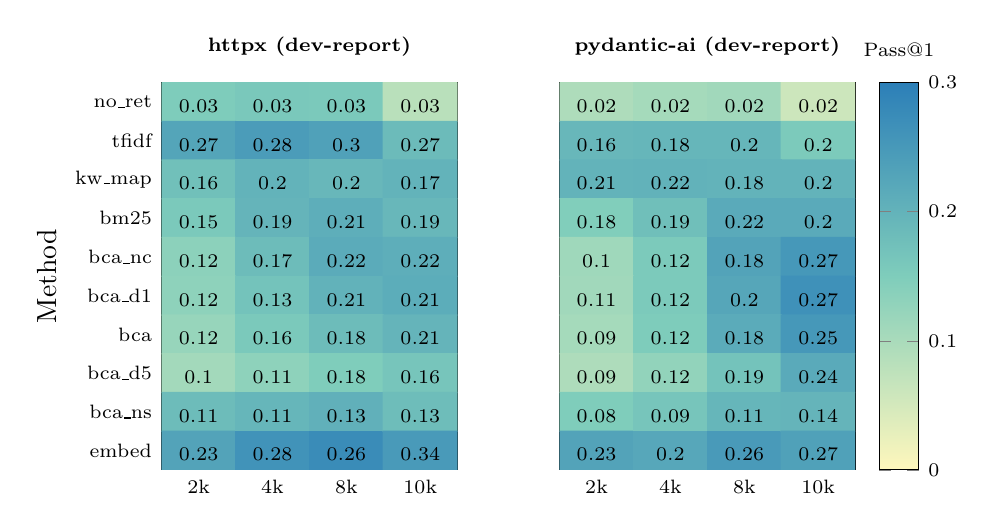
\begin{tikzpicture}
\begin{groupplot}[
  group style={group size=2 by 1, horizontal sep=1.3cm},
  width=0.44\textwidth,
  height=6.5cm,
  y dir=reverse,
  xmin=-0.5, xmax=3.5,
  ymin=-0.5, ymax=9.5,
  xtick={0,1,2,3},
  xticklabels={2k,4k,8k,10k},
  ytick={0,1,2,3,4,5,6,7,8,9},
  yticklabels={no\_ret,tfidf,kw\_map,bm25,bca\_nc,bca\_d1,bca,bca\_d5,bca\_ns,embed},
  point meta min=0.00,
  point meta max=0.30,
  colormap={hmrepo}{rgb255=(255,247,188) rgb255=(127,205,187) rgb255=(44,127,184)},
  nodes near coords,
  every axis plot/.append style={draw=white, line width=0.45pt},
  every node near coord/.append style={
    font=\scriptsize,
    /pgf/number format/fixed,
    /pgf/number format/precision=2,
    text=black,
    anchor=center,
    yshift=-0.35ex
  },
  tick label style={font=\scriptsize},
  title style={font=\scriptsize\bfseries},
]
\nextgroupplot[title={httpx (dev-report)}, ylabel={Method}]
\addplot[
  matrix plot*,
  shader=flat,
  mesh/cols=4,
  point meta=explicit,
] coordinates {
  (0,0) [0.03] (1,0) [0.03] (2,0) [0.03] (3,0) [0.03]
  (0,1) [0.27] (1,1) [0.28] (2,1) [0.30] (3,1) [0.27]
  (0,2) [0.16] (1,2) [0.20] (2,2) [0.20] (3,2) [0.17]
  (0,3) [0.15] (1,3) [0.19] (2,3) [0.21] (3,3) [0.19]
  (0,4) [0.12] (1,4) [0.17] (2,4) [0.22] (3,4) [0.22]
  (0,5) [0.12] (1,5) [0.13] (2,5) [0.21] (3,5) [0.21]
  (0,6) [0.12] (1,6) [0.16] (2,6) [0.18] (3,6) [0.21]
  (0,7) [0.10] (1,7) [0.11] (2,7) [0.18] (3,7) [0.16]
  (0,8) [0.11] (1,8) [0.11] (2,8) [0.13] (3,8) [0.13]
  (0,9) [0.23] (1,9) [0.28] (2,9) [0.26] (3,9) [0.34]
};

\nextgroupplot[title={pydantic-ai (dev-report)}, yticklabels={}, colorbar,
  colorbar style={
    title={Pass@1},
    title style={font=\scriptsize},
    yticklabel style={font=\scriptsize},
    scaled y ticks=false,
    y dir=normal,
    every node near coord/.style={text opacity=0},
  }]
\addplot[
  matrix plot*,
  shader=flat,
  mesh/cols=4,
  point meta=explicit,
] coordinates {
  (0,0) [0.02] (1,0) [0.02] (2,0) [0.02] (3,0) [0.02]
  (0,1) [0.16] (1,1) [0.18] (2,1) [0.20] (3,1) [0.20]
  (0,2) [0.21] (1,2) [0.22] (2,2) [0.18] (3,2) [0.20]
  (0,3) [0.18] (1,3) [0.19] (2,3) [0.22] (3,3) [0.20]
  (0,4) [0.10] (1,4) [0.12] (2,4) [0.18] (3,4) [0.27]
  (0,5) [0.11] (1,5) [0.12] (2,5) [0.20] (3,5) [0.27]
  (0,6) [0.09] (1,6) [0.12] (2,6) [0.18] (3,6) [0.25]
  (0,7) [0.09] (1,7) [0.12] (2,7) [0.19] (3,7) [0.24]
  (0,8) [0.08] (1,8) [0.09] (2,8) [0.11] (3,8) [0.14]
  (0,9) [0.23] (1,9) [0.20] (2,9) [0.26] (3,9) [0.27]
};
\end{groupplot}
\end{tikzpicture}
\caption{Dev-report pass@1 heatmaps by repository. TF-IDF dominates on httpx, while BCA variants become competitive or better at higher budgets on pydantic-ai.}
\label{fig:repo-devreport-heatmaps}
\end{figure}

The repository heatmaps show different budget elasticity.
On httpx, TF-IDF leads at lower budgets while embedding surpasses it at $\B{10\text{k}}$ (0.34 vs.\ 0.27); graph variants mostly close gaps without overtaking.
On pydantic-ai, BCA variants improve more steeply with budget and overtake TF-IDF at \(\B{10\text{k}}\), consistent with a larger codebase where structural context is more useful.

\begin{figure}[H]
\centering
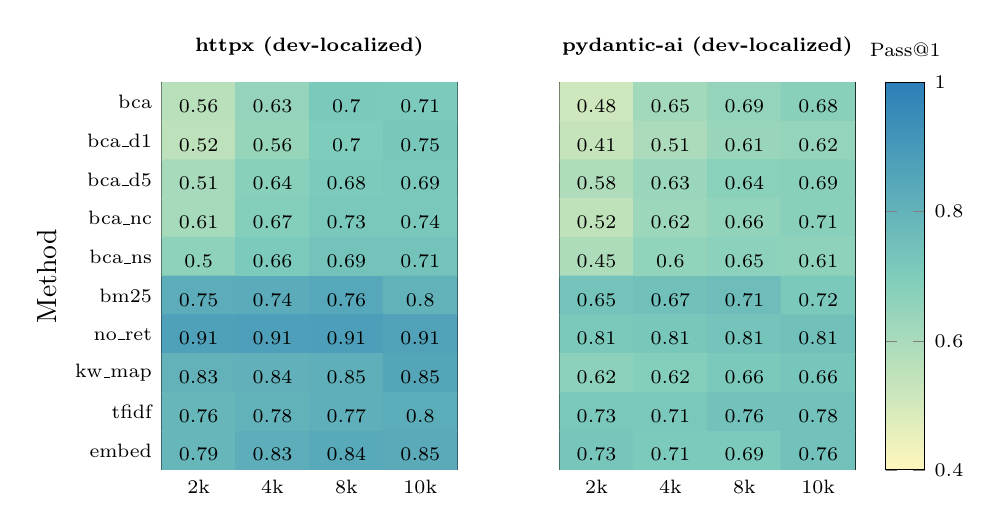
\begin{tikzpicture}
\begin{groupplot}[
  group style={group size=2 by 1, horizontal sep=1.3cm},
  width=0.44\textwidth,
  height=6.5cm,
  y dir=reverse,
  xmin=-0.5, xmax=3.5,
  ymin=-0.5, ymax=9.5,
  xtick={0,1,2,3},
  xticklabels={2k,4k,8k,10k},
  ytick={0,1,2,3,4,5,6,7,8,9},
  yticklabels={bca,bca\_d1,bca\_d5,bca\_nc,bca\_ns,bm25,no\_ret,kw\_map,tfidf,embed},
  point meta min=0.40,
  point meta max=1.00,
  colormap={hmrepoex}{rgb255=(255,247,188) rgb255=(127,205,187) rgb255=(44,127,184)},
  nodes near coords,
  every axis plot/.append style={draw=white, line width=0.45pt},
  every node near coord/.append style={
    font=\scriptsize,
    /pgf/number format/fixed,
    /pgf/number format/precision=2,
    text=black,
    anchor=center,
    yshift=-0.35ex
  },
  tick label style={font=\scriptsize},
  title style={font=\scriptsize\bfseries},
]
\nextgroupplot[title={httpx (dev-localized)}, ylabel={Method}]
\addplot[
  matrix plot*,
  shader=flat,
  mesh/cols=4,
  point meta=explicit,
] coordinates {
  (0,0) [0.56] (1,0) [0.63] (2,0) [0.70] (3,0) [0.71]
  (0,1) [0.52] (1,1) [0.56] (2,1) [0.70] (3,1) [0.75]
  (0,2) [0.51] (1,2) [0.64] (2,2) [0.68] (3,2) [0.69]
  (0,3) [0.61] (1,3) [0.67] (2,3) [0.73] (3,3) [0.74]
  (0,4) [0.50] (1,4) [0.66] (2,4) [0.69] (3,4) [0.71]
  (0,5) [0.75] (1,5) [0.74] (2,5) [0.76] (3,5) [0.80]
  (0,6) [0.91] (1,6) [0.91] (2,6) [0.91] (3,6) [0.91]
  (0,7) [0.83] (1,7) [0.84] (2,7) [0.85] (3,7) [0.85]
  (0,8) [0.76] (1,8) [0.78] (2,8) [0.77] (3,8) [0.80]
  (0,9) [0.79] (1,9) [0.83] (2,9) [0.84] (3,9) [0.85]
};

\nextgroupplot[
  title={pydantic-ai (dev-localized)},
  yticklabels={},
  colorbar,
  colorbar style={
    title={Pass@1},
    title style={font=\scriptsize},
    yticklabel style={font=\scriptsize},
    scaled y ticks=false,
    y dir=normal,
    every node near coord/.style={text opacity=0},
  }
]
\addplot[
  matrix plot*,
  shader=flat,
  mesh/cols=4,
  point meta=explicit,
] coordinates {
  (0,0) [0.48] (1,0) [0.65] (2,0) [0.69] (3,0) [0.68]
  (0,1) [0.41] (1,1) [0.51] (2,1) [0.61] (3,1) [0.62]
  (0,2) [0.58] (1,2) [0.63] (2,2) [0.64] (3,2) [0.69]
  (0,3) [0.52] (1,3) [0.62] (2,3) [0.66] (3,3) [0.71]
  (0,4) [0.45] (1,4) [0.60] (2,4) [0.65] (3,4) [0.61]
  (0,5) [0.65] (1,5) [0.67] (2,5) [0.71] (3,5) [0.72]
  (0,6) [0.81] (1,6) [0.81] (2,6) [0.81] (3,6) [0.81]
  (0,7) [0.62] (1,7) [0.62] (2,7) [0.66] (3,7) [0.66]
  (0,8) [0.73] (1,8) [0.71] (2,8) [0.76] (3,8) [0.78]
  (0,9) [0.73] (1,9) [0.71] (2,9) [0.69] (3,9) [0.76]
};
\end{groupplot}
\end{tikzpicture}
\caption{Dev-localized pass@1 heatmaps by repository. The no-retrieval row is strongest in both repositories, confirming location leakage dominates this tier.}
\label{fig:repo-exact-heatmaps}
\end{figure}

\begin{figure}[H]
\centering
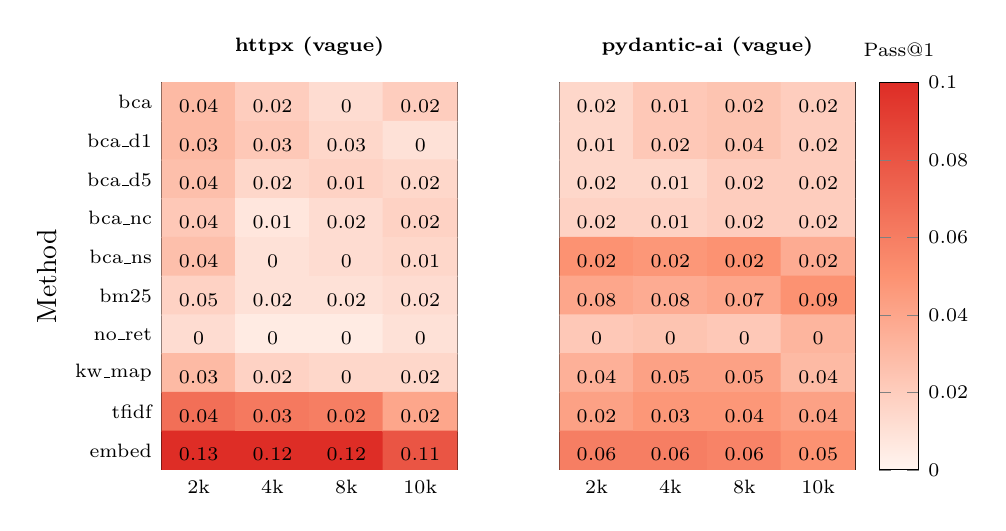
\begin{tikzpicture}
\begin{groupplot}[
  group style={group size=2 by 1, horizontal sep=1.3cm},
  width=0.44\textwidth,
  height=6.5cm,
  y dir=reverse,
  xmin=-0.5, xmax=3.5,
  ymin=-0.5, ymax=9.5,
  xtick={0,1,2,3},
  xticklabels={2k,4k,8k,10k},
  ytick={0,1,2,3,4,5,6,7,8,9},
  yticklabels={bca,bca\_d1,bca\_d5,bca\_nc,bca\_ns,bm25,no\_ret,kw\_map,tfidf,embed},
  point meta min=0.00,
  point meta max=0.10,
  colormap={hmrepovg}{rgb255=(255,245,240) rgb255=(252,146,114) rgb255=(222,45,38)},
  nodes near coords,
  every axis plot/.append style={draw=white, line width=0.45pt},
  every node near coord/.append style={
    font=\scriptsize,
    /pgf/number format/fixed,
    /pgf/number format/precision=2,
    text=black,
    anchor=center,
    yshift=-0.35ex
  },
  tick label style={font=\scriptsize},
  title style={font=\scriptsize\bfseries},
]
\nextgroupplot[title={httpx (vague)}, ylabel={Method}]
\addplot[
  matrix plot*,
  shader=flat,
  mesh/cols=4,
  point meta=explicit,
] coordinates {
  (0,0) [0.04] (1,0) [0.02] (2,0) [0.00] (3,0) [0.02]
  (0,1) [0.03] (1,1) [0.03] (2,1) [0.03] (3,1) [0.00]
  (0,2) [0.04] (1,2) [0.02] (2,2) [0.01] (3,2) [0.02]
  (0,3) [0.04] (1,3) [0.01] (2,3) [0.02] (3,3) [0.02]
  (0,4) [0.04] (1,4) [0.00] (2,4) [0.00] (3,4) [0.01]
  (0,5) [0.05] (1,5) [0.02] (2,5) [0.02] (3,5) [0.02]
  (0,6) [0.00] (1,6) [0.00] (2,6) [0.00] (3,6) [0.00]
  (0,7) [0.03] (1,7) [0.02] (2,7) [0.00] (3,7) [0.02]
  (0,8) [0.04] (1,8) [0.03] (2,8) [0.02] (3,8) [0.02]
  (0,9) [0.13] (1,9) [0.12] (2,9) [0.12] (3,9) [0.11]
};

\nextgroupplot[
  title={pydantic-ai (vague)},
  yticklabels={},
  colorbar,
  colorbar style={
    title={Pass@1},
    title style={font=\scriptsize},
    yticklabel style={font=\scriptsize},
    scaled y ticks=false,
    y dir=normal,
    every node near coord/.style={text opacity=0},
  }
]
\addplot[
  matrix plot*,
  shader=flat,
  mesh/cols=4,
  point meta=explicit,
] coordinates {
  (0,0) [0.02] (1,0) [0.01] (2,0) [0.02] (3,0) [0.02]
  (0,1) [0.01] (1,1) [0.02] (2,1) [0.04] (3,1) [0.02]
  (0,2) [0.02] (1,2) [0.01] (2,2) [0.02] (3,2) [0.02]
  (0,3) [0.02] (1,3) [0.01] (2,3) [0.02] (3,3) [0.02]
  (0,4) [0.02] (1,4) [0.02] (2,4) [0.02] (3,4) [0.02]
  (0,5) [0.08] (1,5) [0.08] (2,5) [0.07] (3,5) [0.09]
  (0,6) [0.00] (1,6) [0.00] (2,6) [0.00] (3,6) [0.00]
  (0,7) [0.04] (1,7) [0.05] (2,7) [0.05] (3,7) [0.04]
  (0,8) [0.02] (1,8) [0.03] (2,8) [0.04] (3,8) [0.04]
  (0,9) [0.06] (1,9) [0.06] (2,9) [0.06] (3,9) [0.05]
};
\end{groupplot}
\end{tikzpicture}
\caption{Vague-tier pass@1 heatmaps by repository. Both repositories remain low-accuracy overall, with bm25 comparatively stronger on pydantic-ai.}
\label{fig:repo-vague-heatmaps}
\end{figure}

These additional repository heatmaps show the same tier asymmetry seen in the main text:
dev-localized is broadly high regardless of retrieval method, while vague stays near-zero with small method differences.

\begin{table}[H]
\centering
\caption{httpx ($N$=117), dev-report, all methods and budgets.}\label{tab:httpx-devreport}
\smallskip
\footnotesize
\begin{tabular}{lcccc}
\toprule
Method & $\B{2\text{k}}$ & $\B{4\text{k}}$ & $\B{8\text{k}}$ & $\B{10\text{k}}$ \\
\midrule
\textsc{bca}              & 0.12 & 0.16 & 0.18 & 0.21 \\
\textsc{bca\_d1}          & 0.12 & 0.13 & 0.21 & 0.21 \\
\textsc{bca\_d5}          & 0.10 & 0.11 & 0.18 & 0.16 \\
\textsc{bca\_no\_closure} & 0.12 & 0.17 & 0.22 & 0.22 \\
\textsc{bca\_no\_scoring} & 0.11 & 0.11 & 0.13 & 0.13 \\
\textsc{bm25}             & 0.15 & 0.19 & 0.21 & 0.19 \\
\textsc{no\_retrieval}    & 0.03 & 0.03 & 0.03 & 0.03 \\
\textsc{keyword\_map}        & 0.16 & 0.20 & 0.20 & 0.17 \\
\textsc{tfidf}           & 0.27 & 0.28 & 0.30 & 0.27 \\
\textsc{embedding}       & 0.23 & 0.28 & 0.26 & 0.34 \\
\bottomrule
\end{tabular}
\end{table}

\begin{table}[H]
\centering
\caption{pydantic-ai ($N$=128), dev-report, all methods and budgets.}\label{tab:pydantic-devreport}
\smallskip
\footnotesize
\begin{tabular}{lcccc}
\toprule
Method & $\B{2\text{k}}$ & $\B{4\text{k}}$ & $\B{8\text{k}}$ & $\B{10\text{k}}$ \\
\midrule
\textsc{bca}              & 0.09 & 0.12 & 0.18 & 0.25 \\
\textsc{bca\_d1}          & 0.11 & 0.12 & 0.20 & 0.27 \\
\textsc{bca\_d5}          & 0.09 & 0.12 & 0.19 & 0.24 \\
\textsc{bca\_no\_closure} & 0.10 & 0.12 & 0.18 & 0.27 \\
\textsc{bca\_no\_scoring} & 0.08 & 0.09 & 0.11 & 0.14 \\
\textsc{bm25}             & 0.18 & 0.19 & 0.22 & 0.20 \\
\textsc{no\_retrieval}    & 0.02 & 0.02 & 0.02 & 0.02 \\
\textsc{keyword\_map}        & 0.21 & 0.22 & 0.18 & 0.20 \\
\textsc{tfidf}           & 0.16 & 0.18 & 0.20 & 0.20 \\
\textsc{embedding}       & 0.23 & 0.20 & 0.26 & 0.27 \\
\bottomrule
\end{tabular}
\end{table}

\begin{table}[H]
\centering
\caption{httpx ($N$=117), dev-localized, all methods and budgets.}\label{tab:httpx-exact}
\smallskip
\footnotesize
\begin{tabular}{lcccc}
\toprule
Method & $\B{2\text{k}}$ & $\B{4\text{k}}$ & $\B{8\text{k}}$ & $\B{10\text{k}}$ \\
\midrule
\textsc{bca}              & 0.56 & 0.63 & 0.70 & 0.71 \\
\textsc{bca\_d1}          & 0.52 & 0.56 & 0.70 & 0.75 \\
\textsc{bca\_d5}          & 0.51 & 0.64 & 0.68 & 0.69 \\
\textsc{bca\_no\_closure} & 0.61 & 0.67 & 0.73 & 0.74 \\
\textsc{bca\_no\_scoring} & 0.50 & 0.66 & 0.69 & 0.71 \\
\textsc{bm25}             & 0.75 & 0.74 & 0.76 & 0.80 \\
\textsc{no\_retrieval}    & 0.91 & 0.91 & 0.91 & 0.91 \\
\textsc{keyword\_map}        & 0.83 & 0.84 & 0.85 & 0.85 \\
\textsc{tfidf}           & 0.76 & 0.78 & 0.77 & 0.80 \\
\textsc{embedding}       & 0.79 & 0.83 & 0.84 & 0.85 \\
\bottomrule
\end{tabular}
\end{table}

\begin{table}[H]
\centering
\caption{pydantic-ai ($N$=128), dev-localized, all methods and budgets.}\label{tab:pydantic-exact}
\smallskip
\footnotesize
\begin{tabular}{lcccc}
\toprule
Method & $\B{2\text{k}}$ & $\B{4\text{k}}$ & $\B{8\text{k}}$ & $\B{10\text{k}}$ \\
\midrule
\textsc{bca}              & 0.48 & 0.65 & 0.69 & 0.68 \\
\textsc{bca\_d1}          & 0.41 & 0.51 & 0.61 & 0.62 \\
\textsc{bca\_d5}          & 0.58 & 0.63 & 0.64 & 0.69 \\
\textsc{bca\_no\_closure} & 0.52 & 0.62 & 0.66 & 0.71 \\
\textsc{bca\_no\_scoring} & 0.45 & 0.60 & 0.65 & 0.61 \\
\textsc{bm25}             & 0.65 & 0.67 & 0.71 & 0.72 \\
\textsc{no\_retrieval}    & 0.81 & 0.81 & 0.81 & 0.81 \\
\textsc{keyword\_map}        & 0.62 & 0.62 & 0.66 & 0.66 \\
\textsc{tfidf}           & 0.73 & 0.71 & 0.76 & 0.78 \\
\textsc{embedding}       & 0.73 & 0.71 & 0.69 & 0.76 \\
\bottomrule
\end{tabular}
\end{table}

\begin{table}[H]
\centering
\caption{httpx ($N$=117), vague, all methods and budgets.}\label{tab:httpx-vague}
\smallskip
\footnotesize
\begin{tabular}{lcccc}
\toprule
Method & $\B{2\text{k}}$ & $\B{4\text{k}}$ & $\B{8\text{k}}$ & $\B{10\text{k}}$ \\
\midrule
\textsc{bca}              & 0.04 & 0.02 & 0.00 & 0.02 \\
\textsc{bca\_d1}          & 0.03 & 0.03 & 0.03 & 0.00 \\
\textsc{bca\_d5}          & 0.04 & 0.02 & 0.01 & 0.02 \\
\textsc{bca\_no\_closure} & 0.04 & 0.01 & 0.02 & 0.02 \\
\textsc{bca\_no\_scoring} & 0.04 & 0.00 & 0.00 & 0.01 \\
\textsc{bm25}             & 0.05 & 0.02 & 0.02 & 0.02 \\
\textsc{no\_retrieval}    & 0.00 & 0.00 & 0.00 & 0.00 \\
\textsc{keyword\_map}        & 0.03 & 0.02 & 0.00 & 0.02 \\
\textsc{tfidf}           & 0.04 & 0.03 & 0.02 & 0.02 \\
\textsc{embedding}       & 0.13 & 0.12 & 0.12 & 0.11 \\
\bottomrule
\end{tabular}
\end{table}

\begin{table}[H]
\centering
\caption{pydantic-ai ($N$=128), vague, all methods and budgets.}\label{tab:pydantic-vague}
\smallskip
\footnotesize
\begin{tabular}{lcccc}
\toprule
Method & $\B{2\text{k}}$ & $\B{4\text{k}}$ & $\B{8\text{k}}$ & $\B{10\text{k}}$ \\
\midrule
\textsc{bca}              & 0.02 & 0.01 & 0.02 & 0.02 \\
\textsc{bca\_d1}          & 0.01 & 0.02 & 0.04 & 0.02 \\
\textsc{bca\_d5}          & 0.02 & 0.01 & 0.02 & 0.02 \\
\textsc{bca\_no\_closure} & 0.02 & 0.01 & 0.02 & 0.02 \\
\textsc{bca\_no\_scoring} & 0.02 & 0.02 & 0.02 & 0.02 \\
\textsc{bm25}             & 0.08 & 0.08 & 0.07 & 0.09 \\
\textsc{no\_retrieval}    & 0.00 & 0.00 & 0.00 & 0.00 \\
\textsc{keyword\_map}        & 0.04 & 0.05 & 0.05 & 0.04 \\
\textsc{tfidf}           & 0.02 & 0.03 & 0.04 & 0.04 \\
\textsc{embedding}       & 0.06 & 0.06 & 0.06 & 0.05 \\
\bottomrule
\end{tabular}
\end{table}

\subsection{Decomposition by Mutation Type}\label{app:muttype-tables}

Tables~\ref{tab:muttype-2k} and~\ref{tab:muttype-10k} report pass@1 by
mutation operator type on dev-report at $\B{2\text{k}}$ and
$\B{10\text{k}}$.  \texttt{none\_check\_swap} is the hardest type across
all methods (best: 16\% at $\B{10\text{k}}$), while
\texttt{constant\_mutation} and \texttt{handcrafted} are the easiest (up to
50\%).
\Cref{fig:muttype-2k-heatmap,fig:muttype-10k-heatmap} summarize the
$\B{2\text{k}}$ and $\B{10\text{k}}$ slices as heatmaps.

\begin{figure}[H]
\centering
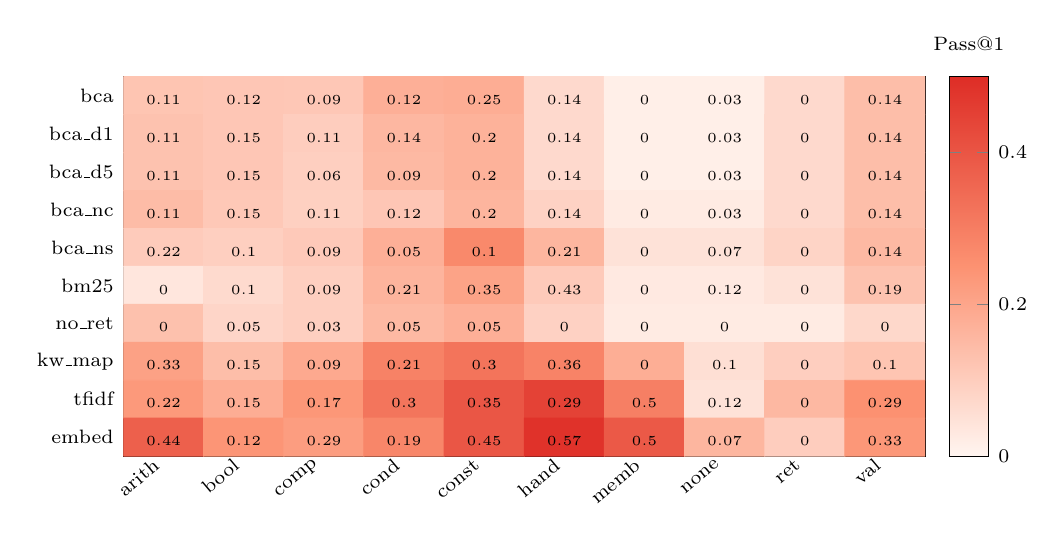
\begin{tikzpicture}
\begin{axis}[
  width=0.97\textwidth,
  height=6.4cm,
  y dir=reverse,
  xmin=-0.5, xmax=9.5,
  ymin=-0.5, ymax=9.5,
  xtick={0,1,2,3,4,5,6,7,8,9},
  xticklabels={arith,bool,comp,cond,const,hand,memb,none,ret,val},
  x tick label style={rotate=40, anchor=east, font=\scriptsize},
  ytick={0,1,2,3,4,5,6,7,8,9},
  yticklabels={bca,bca\_d1,bca\_d5,bca\_nc,bca\_ns,bm25,no\_ret,kw\_map,tfidf,embed},
  point meta min=0.00,
  point meta max=0.50,
  colormap={hmmut}{rgb255=(255,245,240) rgb255=(252,146,114) rgb255=(222,45,38)},
  nodes near coords,
  colorbar,
  colorbar style={
    title={Pass@1},
    title style={font=\scriptsize},
    yticklabel style={font=\scriptsize},
    scaled y ticks=false,
    y dir=normal,
    every node near coord/.style={text opacity=0},
  },
  every axis plot/.append style={draw=white, line width=0.35pt},
  every node near coord/.append style={
    font=\tiny,
    /pgf/number format/fixed,
    /pgf/number format/precision=2,
    text=black,
    anchor=center,
    yshift=-0.35ex
  },
  tick label style={font=\scriptsize},
]
\addplot[
  matrix plot*,
  shader=flat,
  mesh/cols=10,
  point meta=explicit,
] coordinates {
  (0,0) [0.11] (1,0) [0.12] (2,0) [0.09] (3,0) [0.12] (4,0) [0.25] (5,0) [0.14] (6,0) [0.00] (7,0) [0.03] (8,0) [0.00] (9,0) [0.14]
  (0,1) [0.11] (1,1) [0.15] (2,1) [0.11] (3,1) [0.14] (4,1) [0.20] (5,1) [0.14] (6,1) [0.00] (7,1) [0.03] (8,1) [0.00] (9,1) [0.14]
  (0,2) [0.11] (1,2) [0.15] (2,2) [0.06] (3,2) [0.09] (4,2) [0.20] (5,2) [0.14] (6,2) [0.00] (7,2) [0.03] (8,2) [0.00] (9,2) [0.14]
  (0,3) [0.11] (1,3) [0.15] (2,3) [0.11] (3,3) [0.12] (4,3) [0.20] (5,3) [0.14] (6,3) [0.00] (7,3) [0.03] (8,3) [0.00] (9,3) [0.14]
  (0,4) [0.22] (1,4) [0.10] (2,4) [0.09] (3,4) [0.05] (4,4) [0.10] (5,4) [0.21] (6,4) [0.00] (7,4) [0.07] (8,4) [0.00] (9,4) [0.14]
  (0,5) [0.00] (1,5) [0.10] (2,5) [0.09] (3,5) [0.21] (4,5) [0.35] (5,5) [0.43] (6,5) [0.00] (7,5) [0.12] (8,5) [0.00] (9,5) [0.19]
  (0,6) [0.00] (1,6) [0.05] (2,6) [0.03] (3,6) [0.05] (4,6) [0.05] (5,6) [0.00] (6,6) [0.00] (7,6) [0.00] (8,6) [0.00] (9,6) [0.00]
  (0,7) [0.33] (1,7) [0.15] (2,7) [0.09] (3,7) [0.21] (4,7) [0.30] (5,7) [0.36] (6,7) [0.00] (7,7) [0.10] (8,7) [0.00] (9,7) [0.10]
  (0,8) [0.22] (1,8) [0.15] (2,8) [0.17] (3,8) [0.30] (4,8) [0.35] (5,8) [0.29] (6,8) [0.50] (7,8) [0.12] (8,8) [0.00] (9,8) [0.29]
  (0,9) [0.44] (1,9) [0.12] (2,9) [0.29] (3,9) [0.19] (4,9) [0.45] (5,9) [0.57] (6,9) [0.50] (7,9) [0.07] (8,9) [0.00] (9,9) [0.33]
};
\end{axis}
\end{tikzpicture}
\caption{Dev-report mutation-type heatmap at $\B{2\text{k}}$. Lower-budget slice highlights where lexical methods dominate before graph context has room to grow.}
\label{fig:muttype-2k-heatmap}
\end{figure}

\begin{figure}[H]
\centering
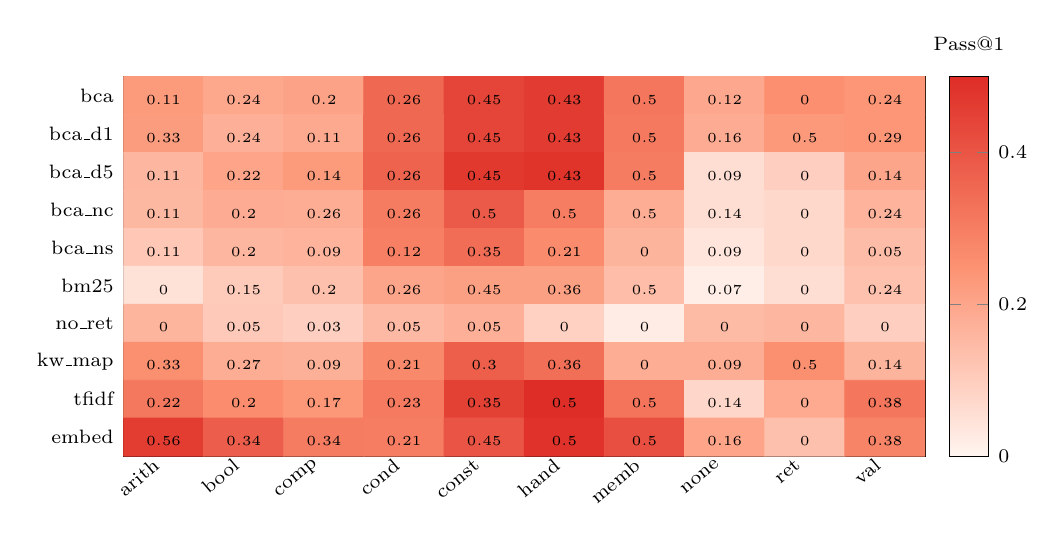
\begin{tikzpicture}
\begin{axis}[
  width=0.97\textwidth,
  height=6.4cm,
  y dir=reverse,
  xmin=-0.5, xmax=9.5,
  ymin=-0.5, ymax=9.5,
  xtick={0,1,2,3,4,5,6,7,8,9},
  xticklabels={arith,bool,comp,cond,const,hand,memb,none,ret,val},
  x tick label style={rotate=40, anchor=east, font=\scriptsize},
  ytick={0,1,2,3,4,5,6,7,8,9},
  yticklabels={bca,bca\_d1,bca\_d5,bca\_nc,bca\_ns,bm25,no\_ret,kw\_map,tfidf,embed},
  point meta min=0.00,
  point meta max=0.50,
  colormap={hmmut}{rgb255=(255,245,240) rgb255=(252,146,114) rgb255=(222,45,38)},
  nodes near coords,
  colorbar,
  colorbar style={
    title={Pass@1},
    title style={font=\scriptsize},
    yticklabel style={font=\scriptsize},
    scaled y ticks=false,
    y dir=normal,
    every node near coord/.style={text opacity=0},
  },
  every axis plot/.append style={draw=white, line width=0.35pt},
  every node near coord/.append style={
    font=\tiny,
    /pgf/number format/fixed,
    /pgf/number format/precision=2,
    text=black,
    anchor=center,
    yshift=-0.35ex
  },
  tick label style={font=\scriptsize},
]
\addplot[
  matrix plot*,
  shader=flat,
  mesh/cols=10,
  point meta=explicit,
] coordinates {
  (0,0) [0.11] (1,0) [0.24] (2,0) [0.20] (3,0) [0.26] (4,0) [0.45] (5,0) [0.43] (6,0) [0.50] (7,0) [0.12] (8,0) [0.00] (9,0) [0.24]
  (0,1) [0.33] (1,1) [0.24] (2,1) [0.11] (3,1) [0.26] (4,1) [0.45] (5,1) [0.43] (6,1) [0.50] (7,1) [0.16] (8,1) [0.50] (9,1) [0.29]
  (0,2) [0.11] (1,2) [0.22] (2,2) [0.14] (3,2) [0.26] (4,2) [0.45] (5,2) [0.43] (6,2) [0.50] (7,2) [0.09] (8,2) [0.00] (9,2) [0.14]
  (0,3) [0.11] (1,3) [0.20] (2,3) [0.26] (3,3) [0.26] (4,3) [0.50] (5,3) [0.50] (6,3) [0.50] (7,3) [0.14] (8,3) [0.00] (9,3) [0.24]
  (0,4) [0.11] (1,4) [0.20] (2,4) [0.09] (3,4) [0.12] (4,4) [0.35] (5,4) [0.21] (6,4) [0.00] (7,4) [0.09] (8,4) [0.00] (9,4) [0.05]
  (0,5) [0.00] (1,5) [0.15] (2,5) [0.20] (3,5) [0.26] (4,5) [0.45] (5,5) [0.36] (6,5) [0.50] (7,5) [0.07] (8,5) [0.00] (9,5) [0.24]
  (0,6) [0.00] (1,6) [0.05] (2,6) [0.03] (3,6) [0.05] (4,6) [0.05] (5,6) [0.00] (6,6) [0.00] (7,6) [0.00] (8,6) [0.00] (9,6) [0.00]
  (0,7) [0.33] (1,7) [0.27] (2,7) [0.09] (3,7) [0.21] (4,7) [0.30] (5,7) [0.36] (6,7) [0.00] (7,7) [0.09] (8,7) [0.50] (9,7) [0.14]
  (0,8) [0.22] (1,8) [0.20] (2,8) [0.17] (3,8) [0.23] (4,8) [0.35] (5,8) [0.50] (6,8) [0.50] (7,8) [0.14] (8,8) [0.00] (9,8) [0.38]
  (0,9) [0.56] (1,9) [0.34] (2,9) [0.34] (3,9) [0.21] (4,9) [0.45] (5,9) [0.50] (6,9) [0.50] (7,9) [0.16] (8,9) [0.00] (9,9) [0.38]
};
\end{axis}
\end{tikzpicture}
\caption{Dev-report mutation-type heatmap at $\B{10\text{k}}$. Columns: arithmetic (\texttt{arith}), boolean (\texttt{bool}), comparison (\texttt{comp}), condition inversion (\texttt{cond}), constant (\texttt{const}), handcrafted (\texttt{hand}), membership (\texttt{memb}), none-check (\texttt{none}), return-value (\texttt{ret}), value-swap (\texttt{val}).}
\label{fig:muttype-10k-heatmap}
\end{figure}

This heatmap highlights two stable patterns that are less obvious in the tables.
\texttt{none\_check\_swap} remains uniformly hard across methods, while \texttt{constant\_mutation} and \texttt{handcrafted} are consistently easier.
It also reinforces the ablation result that removing BCA scoring (\textsc{bca\_no\_scoring}) degrades performance across most mutation types.
Comparing \Cref{fig:muttype-2k-heatmap} with \Cref{fig:muttype-10k-heatmap}
also shows where additional budget helps most: medium-complexity operators
(\texttt{comp}, \texttt{cond}, \texttt{val}) brighten for several BCA variants,
while \texttt{none\_check\_swap} remains dark across both budgets.

\begin{table}[H]
\centering
\caption{Pass@1 by mutation type, dev-report at $\B{2\text{k}}$, all methods.}\label{tab:muttype-2k}
\smallskip
\resizebox{\columnwidth}{!}{%
\begin{tabular}{l cccccccccc r}
\toprule
Mutation type & bca & bca\_d1 & bca\_d5 & bca\_nc & bca\_ns & bm25 & no\_ret & kw\_map & tfidf & embed & $N$ \\
\midrule
arithmetic\_swap                 & 0.11 & 0.11 & 0.11 & 0.11 & 0.22 & 0.00 & 0.00 & 0.33 & 0.22 & 0.44 &  9 \\
boolean\_flip                    & 0.12 & 0.15 & 0.15 & 0.15 & 0.10 & 0.10 & 0.05 & 0.29 & 0.15 & 0.12 & 41 \\
comparison\_swap                 & 0.09 & 0.11 & 0.06 & 0.11 & 0.09 & 0.09 & 0.03 & 0.09 & 0.17 & 0.29 & 35 \\
condition\_inversion             & 0.12 & 0.14 & 0.09 & 0.12 & 0.05 & 0.21 & 0.05 & 0.21 & 0.30 & 0.19 & 43 \\
constant\_mutation               & 0.25 & 0.20 & 0.20 & 0.20 & 0.10 & 0.35 & 0.05 & 0.30 & 0.35 & 0.45 & 20 \\
handcrafted                     & 0.14 & 0.14 & 0.14 & 0.14 & 0.21 & 0.43 & 0.00 & 0.36 & 0.29 & 0.57 & 14 \\
membership\_swap                 & 0.00 & 0.00 & 0.00 & 0.00 & 0.00 & 0.00 & 0.00 & 0.00 & 0.50 & 0.50 &  2 \\
none\_check\_swap                & 0.03 & 0.03 & 0.03 & 0.03 & 0.07 & 0.12 & 0.00 & 0.10 & 0.12 & 0.07 & 58 \\
return\_value\_swap              & 0.00 & 0.00 & 0.00 & 0.00 & 0.00 & 0.00 & 0.00 & 0.00 & 0.00 & 0.00 &  2 \\
value\_swap                      & 0.14 & 0.14 & 0.14 & 0.14 & 0.14 & 0.19 & 0.00 & 0.10 & 0.29 & 0.33 & 21 \\
\bottomrule
\end{tabular}%
}
\end{table}

\begin{table}[H]
\centering
\caption{Pass@1 by mutation type, dev-report at $\B{10\text{k}}$, all methods.}\label{tab:muttype-10k}
\smallskip
\resizebox{\columnwidth}{!}{%
\begin{tabular}{l cccccccccc r}
\toprule
Mutation type & bca & bca\_d1 & bca\_d5 & bca\_nc & bca\_ns & bm25 & no\_ret & kw\_map & tfidf & embed & $N$ \\
\midrule
arithmetic\_swap                 & 0.11 & 0.33 & 0.11 & 0.11 & 0.11 & 0.00 & 0.00 & 0.33 & 0.22 & 0.56 &  9 \\
boolean\_flip                    & 0.24 & 0.24 & 0.22 & 0.20 & 0.20 & 0.15 & 0.05 & 0.27 & 0.20 & 0.34 & 41 \\
comparison\_swap                 & 0.20 & 0.11 & 0.14 & 0.26 & 0.09 & 0.20 & 0.03 & 0.09 & 0.17 & 0.34 & 35 \\
condition\_inversion             & 0.26 & 0.26 & 0.26 & 0.26 & 0.12 & 0.26 & 0.05 & 0.21 & 0.23 & 0.21 & 43 \\
constant\_mutation               & 0.45 & 0.45 & 0.45 & 0.50 & 0.35 & 0.45 & 0.05 & 0.30 & 0.35 & 0.45 & 20 \\
handcrafted                     & 0.43 & 0.43 & 0.43 & 0.50 & 0.21 & 0.36 & 0.00 & 0.36 & 0.50 & 0.50 & 14 \\
membership\_swap                 & 0.50 & 0.50 & 0.50 & 0.50 & 0.00 & 0.50 & 0.00 & 0.00 & 0.50 & 0.50 &  2 \\
none\_check\_swap                & 0.12 & 0.16 & 0.09 & 0.14 & 0.09 & 0.07 & 0.00 & 0.09 & 0.14 & 0.16 & 58 \\
return\_value\_swap              & 0.00 & 0.50 & 0.00 & 0.00 & 0.00 & 0.00 & 0.00 & 0.50 & 0.00 & 0.00 &  2 \\
value\_swap                      & 0.24 & 0.29 & 0.14 & 0.24 & 0.05 & 0.24 & 0.00 & 0.14 & 0.38 & 0.38 & 21 \\
\bottomrule
\end{tabular}%
}
\end{table}

\subsection{Conditional Bins}\label{app:conditional-bins}

These tables decompose pass@1 by three conditioning variables.
Tables~\ref{tab:bin-ident-exact}--\ref{tab:bin-ident-vague}: identifier
density (whether the query contains code identifiers).
Tables~\ref{tab:bin-hops-2k}--\ref{tab:bin-hops-vague}: BCA seed-to-mutation
hop distance.
Tables~\ref{tab:bin-size-2k}--\ref{tab:bin-size-vague}: mutation function
size in lines.
The dev-report slices are summarized visually in
\Cref{fig:bin-hops-heatmap,fig:bin-size-heatmap}.

\begin{figure}[H]
\centering
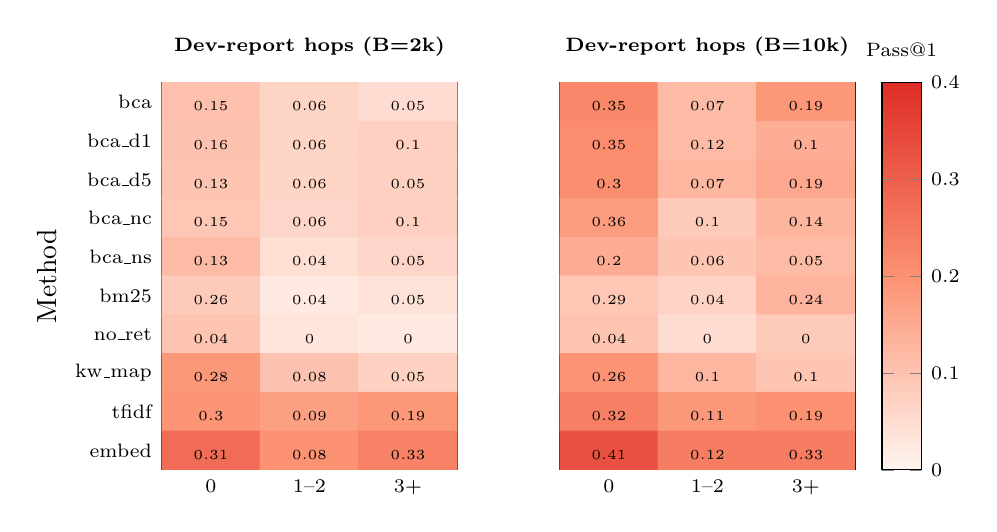
\begin{tikzpicture}
\begin{groupplot}[
  group style={group size=2 by 1, horizontal sep=1.3cm},
  width=0.44\textwidth,
  height=6.5cm,
  y dir=reverse,
  xmin=-0.5, xmax=2.5,
  ymin=-0.5, ymax=9.5,
  xtick={0,1,2},
  xticklabels={0,1--2,3+},
  ytick={0,1,2,3,4,5,6,7,8,9},
  yticklabels={bca,bca\_d1,bca\_d5,bca\_nc,bca\_ns,bm25,no\_ret,kw\_map,tfidf,embed},
  point meta min=0.00,
  point meta max=0.40,
  colormap={hmbinshop}{rgb255=(255,245,240) rgb255=(252,146,114) rgb255=(222,45,38)},
  nodes near coords,
  every axis plot/.append style={draw=white, line width=0.45pt},
  every node near coord/.append style={
    font=\tiny,
    /pgf/number format/fixed,
    /pgf/number format/precision=2,
    text=black,
    anchor=center,
    yshift=-0.35ex
  },
  tick label style={font=\scriptsize},
  title style={font=\scriptsize\bfseries},
]
\nextgroupplot[title={Dev-report hops (\B{2\text{k}})}, ylabel={Method}]
\addplot[
  matrix plot*,
  shader=flat,
  mesh/cols=3,
  point meta=explicit,
] coordinates {
  (0,0) [0.15] (1,0) [0.06] (2,0) [0.05]
  (0,1) [0.16] (1,1) [0.06] (2,1) [0.10]
  (0,2) [0.13] (1,2) [0.06] (2,2) [0.05]
  (0,3) [0.15] (1,3) [0.06] (2,3) [0.10]
  (0,4) [0.13] (1,4) [0.04] (2,4) [0.05]
  (0,5) [0.26] (1,5) [0.04] (2,5) [0.05]
  (0,6) [0.04] (1,6) [0.00] (2,6) [0.00]
  (0,7) [0.28] (1,7) [0.08] (2,7) [0.05]
  (0,8) [0.30] (1,8) [0.09] (2,8) [0.19]
  (0,9) [0.31] (1,9) [0.08] (2,9) [0.33]
};

\nextgroupplot[
  title={Dev-report hops (\B{10\text{k}})},
  yticklabels={},
  colorbar,
  colorbar style={
    title={Pass@1},
    title style={font=\scriptsize},
    yticklabel style={font=\scriptsize},
    scaled y ticks=false,
    y dir=normal,
    every node near coord/.style={text opacity=0},
  }
]
\addplot[
  matrix plot*,
  shader=flat,
  mesh/cols=3,
  point meta=explicit,
] coordinates {
  (0,0) [0.35] (1,0) [0.07] (2,0) [0.19]
  (0,1) [0.35] (1,1) [0.12] (2,1) [0.10]
  (0,2) [0.30] (1,2) [0.07] (2,2) [0.19]
  (0,3) [0.36] (1,3) [0.10] (2,3) [0.14]
  (0,4) [0.20] (1,4) [0.06] (2,4) [0.05]
  (0,5) [0.29] (1,5) [0.04] (2,5) [0.24]
  (0,6) [0.04] (1,6) [0.00] (2,6) [0.00]
  (0,7) [0.26] (1,7) [0.10] (2,7) [0.10]
  (0,8) [0.32] (1,8) [0.11] (2,8) [0.19]
  (0,9) [0.41] (1,9) [0.12] (2,9) [0.33]
};
\end{groupplot}
\end{tikzpicture}
\caption{Conditional-bin heatmaps for hop distance on dev-report. Budget primarily boosts hop-0 cells; 1--2 hop bins remain low across methods.}
\label{fig:bin-hops-heatmap}
\end{figure}

\begin{figure}[H]
\centering
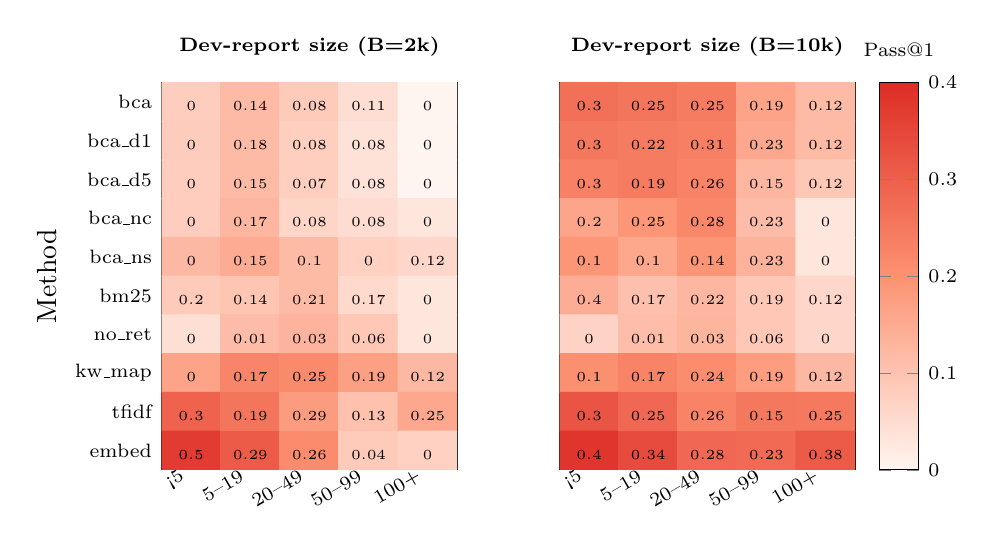
\begin{tikzpicture}
\begin{groupplot}[
  group style={group size=2 by 1, horizontal sep=1.3cm},
  width=0.44\textwidth,
  height=6.5cm,
  y dir=reverse,
  xmin=-0.5, xmax=4.5,
  ymin=-0.5, ymax=9.5,
  xtick={0,1,2,3,4},
  xticklabels={<5,5--19,20--49,50--99,100+},
  x tick label style={rotate=30, anchor=east, font=\scriptsize},
  ytick={0,1,2,3,4,5,6,7,8,9},
  yticklabels={bca,bca\_d1,bca\_d5,bca\_nc,bca\_ns,bm25,no\_ret,kw\_map,tfidf,embed},
  point meta min=0.00,
  point meta max=0.40,
  colormap={hmbinsize}{rgb255=(255,245,240) rgb255=(252,146,114) rgb255=(222,45,38)},
  nodes near coords,
  every axis plot/.append style={draw=white, line width=0.45pt},
  every node near coord/.append style={
    font=\tiny,
    /pgf/number format/fixed,
    /pgf/number format/precision=2,
    text=black,
    anchor=center,
    yshift=-0.35ex
  },
  tick label style={font=\scriptsize},
  title style={font=\scriptsize\bfseries},
]
\nextgroupplot[title={Dev-report size (\B{2\text{k}})}, ylabel={Method}]
\addplot[
  matrix plot*,
  shader=flat,
  mesh/cols=5,
  point meta=explicit,
] coordinates {
  (0,0) [0.00] (1,0) [0.14] (2,0) [0.08] (3,0) [0.11] (4,0) [0.00]
  (0,1) [0.00] (1,1) [0.18] (2,1) [0.08] (3,1) [0.08] (4,1) [0.00]
  (0,2) [0.00] (1,2) [0.15] (2,2) [0.07] (3,2) [0.08] (4,2) [0.00]
  (0,3) [0.00] (1,3) [0.17] (2,3) [0.08] (3,3) [0.08] (4,3) [0.00]
  (0,4) [0.00] (1,4) [0.15] (2,4) [0.10] (3,4) [0.00] (4,4) [0.12]
  (0,5) [0.20] (1,5) [0.14] (2,5) [0.21] (3,5) [0.17] (4,5) [0.00]
  (0,6) [0.00] (1,6) [0.01] (2,6) [0.03] (3,6) [0.06] (4,6) [0.00]
  (0,7) [0.00] (1,7) [0.17] (2,7) [0.25] (3,7) [0.19] (4,7) [0.12]
  (0,8) [0.30] (1,8) [0.19] (2,8) [0.29] (3,8) [0.13] (4,8) [0.25]
  (0,9) [0.50] (1,9) [0.29] (2,9) [0.26] (3,9) [0.04] (4,9) [0.00]
};

\nextgroupplot[
  title={Dev-report size (\B{10\text{k}})},
  yticklabels={},
  colorbar,
  colorbar style={
    title={Pass@1},
    title style={font=\scriptsize},
    yticklabel style={font=\scriptsize},
    scaled y ticks=false,
    y dir=normal,
    every node near coord/.style={text opacity=0},
  }
]
\addplot[
  matrix plot*,
  shader=flat,
  mesh/cols=5,
  point meta=explicit,
] coordinates {
  (0,0) [0.30] (1,0) [0.25] (2,0) [0.25] (3,0) [0.19] (4,0) [0.12]
  (0,1) [0.30] (1,1) [0.22] (2,1) [0.31] (3,1) [0.23] (4,1) [0.12]
  (0,2) [0.30] (1,2) [0.19] (2,2) [0.26] (3,2) [0.15] (4,2) [0.12]
  (0,3) [0.20] (1,3) [0.25] (2,3) [0.28] (3,3) [0.23] (4,3) [0.00]
  (0,4) [0.10] (1,4) [0.10] (2,4) [0.14] (3,4) [0.23] (4,4) [0.00]
  (0,5) [0.40] (1,5) [0.17] (2,5) [0.22] (3,5) [0.19] (4,5) [0.12]
  (0,6) [0.00] (1,6) [0.01] (2,6) [0.03] (3,6) [0.06] (4,6) [0.00]
  (0,7) [0.10] (1,7) [0.17] (2,7) [0.24] (3,7) [0.19] (4,7) [0.12]
  (0,8) [0.30] (1,8) [0.25] (2,8) [0.26] (3,8) [0.15] (4,8) [0.25]
  (0,9) [0.40] (1,9) [0.34] (2,9) [0.28] (3,9) [0.23] (4,9) [0.38]
};
\end{groupplot}
\end{tikzpicture}
\caption{Conditional-bin heatmaps for mutation-size bands on dev-report. Budget gains are broad but uneven, with the largest improvements in small/medium functions.}
\label{fig:bin-size-heatmap}
\end{figure}

The conditional-bin heatmaps make two interactions visually explicit:
budget mostly helps when structural access is already good (hop-0), and it
helps most in smaller-to-medium mutation scopes rather than uniformly across
all function-size bins.

\begin{table}[H]
\centering
\caption{Pass@1 by identifier density, dev-localized, all methods.}\label{tab:bin-ident-exact}
\smallskip
\resizebox{\columnwidth}{!}{%
\begin{tabular}{l cccccccccc r}
\toprule
Identifier density & bca & bca\_d1 & bca\_d5 & bca\_nc & bca\_ns & bm25 & no\_ret & kw\_map & tfidf & embed & $N$ \\
\midrule
\multicolumn{12}{l}{\textit{$\B{2\text{k}}$}} \\
positive & 0.50 & 0.47 & 0.55 & 0.56 & 0.47 & 0.71 & 0.81 & 0.73 & 0.77 & 0.74 & 150 \\
zero     & 0.56 & 0.45 & 0.54 & 0.57 & 0.48 & 0.68 & 0.95 & 0.69 & 0.69 & 0.79 &  95 \\
\midrule
\multicolumn{12}{l}{\textit{$\B{10\text{k}}$}} \\
positive & 0.69 & 0.72 & 0.67 & 0.72 & 0.63 & 0.78 & 0.81 & 0.79 & 0.81 & 0.79 & 150 \\
zero     & 0.71 & 0.63 & 0.73 & 0.73 & 0.71 & 0.73 & 0.95 & 0.67 & 0.77 & 0.82 &  95 \\
\bottomrule
\end{tabular}%
}
\end{table}

\begin{table}[H]
\centering
\caption{Pass@1 by identifier density, dev-report, all methods. All dev-report queries have identifiers (traceback tokens).}\label{tab:bin-ident-devreport}
\smallskip
\resizebox{\columnwidth}{!}{%
\begin{tabular}{l cccccccccc r}
\toprule
Identifier density & bca & bca\_d1 & bca\_d5 & bca\_nc & bca\_ns & bm25 & no\_ret & kw\_map & tfidf & embed & $N$ \\
\midrule
\multicolumn{12}{l}{\textit{$\B{2\text{k}}$}} \\
positive & 0.11 & 0.11 & 0.10 & 0.11 & 0.09 & 0.16 & 0.02 & 0.19 & 0.21 & 0.23 & 245 \\
\midrule
\multicolumn{12}{l}{\textit{$\B{10\text{k}}$}} \\
positive & 0.23 & 0.24 & 0.20 & 0.24 & 0.13 & 0.20 & 0.02 & 0.19 & 0.23 & 0.30 & 245 \\
\bottomrule
\end{tabular}%
}
\end{table}

\begin{table}[H]
\centering
\caption{Pass@1 by identifier density, vague, all methods. Only 4 vague queries contain identifiers.}\label{tab:bin-ident-vague}
\smallskip
\resizebox{\columnwidth}{!}{%
\begin{tabular}{l cccccccccc r}
\toprule
Identifier density & bca & bca\_d1 & bca\_d5 & bca\_nc & bca\_ns & bm25 & emb & no\_ret & kw\_map & tfidf & $N$ \\
\midrule
\multicolumn{12}{l}{\textit{$\B{2\text{k}}$}} \\
positive & 0.00 & 0.00 & 0.00 & 0.00 & 0.25 & 0.50 & 0.75 & 0.00 & 0.25 & 0.00 &   4 \\
zero     & 0.03 & 0.02 & 0.03 & 0.03 & 0.03 & 0.06 & 0.08 & 0.00 & 0.03 & 0.03 & 241 \\
\midrule
\multicolumn{12}{l}{\textit{$\B{10\text{k}}$}} \\
positive & 0.25 & 0.50 & 0.25 & 0.25 & 0.25 & 0.50 & 0.75 & 0.00 & 0.25 & 0.50 &   4 \\
zero     & 0.02 & 0.00 & 0.01 & 0.01 & 0.01 & 0.05 & 0.07 & 0.00 & 0.02 & 0.02 & 241 \\
\bottomrule
\end{tabular}%
}
\end{table}

\begin{table}[H]
\centering
\caption{Pass@1 by hop distance, dev-report at $\B{2\text{k}}$, all methods.}\label{tab:bin-hops-2k}
\smallskip
\resizebox{\columnwidth}{!}{%
\begin{tabular}{l cccccccccc r}
\toprule
Hops & bca & bca\_d1 & bca\_d5 & bca\_nc & bca\_ns & bm25 & no\_ret & kw\_map & tfidf & embed & $N$ \\
\midrule
0         & 0.15 & 0.16 & 0.13 & 0.15 & 0.13 & 0.26 & 0.04 & 0.28 & 0.30 & 0.31 & 135 \\
1--2      & 0.06 & 0.06 & 0.06 & 0.06 & 0.04 & 0.04 & 0.00 & 0.08 & 0.09 & 0.08 &  89 \\
3+        & 0.05 & 0.10 & 0.05 & 0.10 & 0.05 & 0.05 & 0.00 & 0.05 & 0.19 & 0.33 &  21 \\
\bottomrule
\end{tabular}%
}
\end{table}

\begin{table}[H]
\centering
\caption{Pass@1 by hop distance, dev-report at $\B{10\text{k}}$, all methods.}\label{tab:bin-hops-10k}
\smallskip
\resizebox{\columnwidth}{!}{%
\begin{tabular}{l cccccccccc r}
\toprule
Hops & bca & bca\_d1 & bca\_d5 & bca\_nc & bca\_ns & bm25 & no\_ret & kw\_map & tfidf & embed & $N$ \\
\midrule
0         & 0.35 & 0.35 & 0.30 & 0.36 & 0.20 & 0.29 & 0.04 & 0.26 & 0.32 & 0.41 & 135 \\
1--2      & 0.07 & 0.12 & 0.07 & 0.10 & 0.06 & 0.04 & 0.00 & 0.10 & 0.11 & 0.12 &  89 \\
3+        & 0.19 & 0.10 & 0.19 & 0.14 & 0.05 & 0.24 & 0.00 & 0.10 & 0.19 & 0.33 &  21 \\
\bottomrule
\end{tabular}%
}
\end{table}

\begin{table}[H]
\centering
\caption{Pass@1 by hop distance, dev-localized, all methods. Nearly all tasks are hop-0.}\label{tab:bin-hops-exact}
\smallskip
\resizebox{\columnwidth}{!}{%
\begin{tabular}{l cccccccccc r}
\toprule
Hops & bca & bca\_d1 & bca\_d5 & bca\_nc & bca\_ns & bm25 & no\_ret & kw\_map & tfidf & embed & $N$ \\
\midrule
\multicolumn{12}{l}{\textit{$\B{2\text{k}}$}} \\
0         & 0.53 & 0.46 & 0.55 & 0.57 & 0.47 & 0.70 & 0.88 & 0.72 & 0.74 & 0.76 & 240 \\
1--2      & 0.50 & 0.75 & 0.75 & 0.50 & 0.50 & 0.25 & 0.00 & 0.50 & 0.75 & 0.75 &   4 \\
unreachable & 0.00 & 0.00 & 0.00 & 0.00 & 1.00 & 1.00 & 0.00 & 1.00 & 1.00 & 1.00 &   1 \\
\midrule
\multicolumn{12}{l}{\textit{$\B{10\text{k}}$}} \\
0         & 0.70 & 0.68 & 0.70 & 0.72 & 0.66 & 0.77 & 0.88 & 0.75 & 0.79 & 0.80 & 240 \\
1--2      & 0.75 & 1.00 & 0.50 & 0.75 & 0.75 & 0.25 & 0.00 & 0.50 & 0.75 & 1.00 &   4 \\
unreachable & 0.00 & 1.00 & 0.00 & 0.00 & 0.00 & 1.00 & 0.00 & 1.00 & 1.00 & 1.00 &   1 \\
\bottomrule
\end{tabular}%
}
\end{table}

\begin{table}[H]
\centering
\caption{Pass@1 by hop distance, vague, all methods. 89\% of tasks are unreachable from vague-query seeds.}\label{tab:bin-hops-vague}
\smallskip
\resizebox{\columnwidth}{!}{%
\begin{tabular}{l cccccccccc r}
\toprule
Hops & bca & bca\_d1 & bca\_d5 & bca\_nc & bca\_ns & bm25 & emb & no\_ret & kw\_map & tfidf & $N$ \\
\midrule
\multicolumn{12}{l}{\textit{$\B{2\text{k}}$}} \\
0         & 0.00 & 0.00 & 0.00 & 0.00 & 0.00 & 0.00 & 0.00 & 0.00 & 0.00 & 0.00 &   3 \\
1--2      & 0.06 & 0.06 & 0.06 & 0.06 & 0.06 & 0.12 & 0.12 & 0.00 & 0.00 & 0.00 &  16 \\
3+        & 0.00 & 0.00 & 0.00 & 0.00 & 0.00 & 0.00 & 0.14 & 0.00 & 0.14 & 0.00 &   7 \\
unreachable & 0.03 & 0.01 & 0.03 & 0.03 & 0.03 & 0.06 & 0.09 & 0.00 & 0.04 & 0.04 & 219 \\
\midrule
\multicolumn{12}{l}{\textit{$\B{10\text{k}}$}} \\
0         & 0.00 & 0.00 & 0.00 & 0.00 & 0.00 & 0.00 & 0.00 & 0.00 & 0.00 & 0.00 &   3 \\
1--2      & 0.06 & 0.06 & 0.06 & 0.06 & 0.06 & 0.12 & 0.12 & 0.00 & 0.00 & 0.06 &  16 \\
3+        & 0.00 & 0.00 & 0.00 & 0.00 & 0.00 & 0.14 & 0.00 & 0.00 & 0.14 & 0.00 &   7 \\
unreachable & 0.02 & 0.01 & 0.01 & 0.01 & 0.01 & 0.05 & 0.08 & 0.00 & 0.03 & 0.03 & 219 \\
\bottomrule
\end{tabular}%
}
\end{table}

\begin{table}[H]
\centering
\caption{Pass@1 by mutation size, dev-report at $\B{2\text{k}}$, all methods.}\label{tab:bin-size-2k}
\smallskip
\resizebox{\columnwidth}{!}{%
\begin{tabular}{l cccccccccc r}
\toprule
Size (lines) & bca & bca\_d1 & bca\_d5 & bca\_nc & bca\_ns & bm25 & no\_ret & kw\_map & tfidf & embed & $N$ \\
\midrule
$<$5       & 0.00 & 0.00 & 0.00 & 0.00 & 0.00 & 0.20 & 0.00 & 0.00 & 0.30 & 0.50 & 10 \\
5--19      & 0.14 & 0.18 & 0.15 & 0.17 & 0.15 & 0.14 & 0.01 & 0.17 & 0.19 & 0.29 & 102 \\
20--49     & 0.08 & 0.08 & 0.07 & 0.08 & 0.10 & 0.21 & 0.03 & 0.25 & 0.29 & 0.26 & 72 \\
50--99     & 0.11 & 0.08 & 0.08 & 0.08 & 0.00 & 0.17 & 0.06 & 0.19 & 0.13 & 0.04 & 53 \\
100+       & 0.00 & 0.00 & 0.00 & 0.00 & 0.12 & 0.00 & 0.00 & 0.12 & 0.25 & 0.00 &  8 \\
\bottomrule
\end{tabular}%
}
\end{table}

\begin{table}[H]
\centering
\caption{Pass@1 by mutation size, dev-report at $\B{10\text{k}}$, all methods.}\label{tab:bin-size-10k}
\smallskip
\resizebox{\columnwidth}{!}{%
\begin{tabular}{l cccccccccc r}
\toprule
Size (lines) & bca & bca\_d1 & bca\_d5 & bca\_nc & bca\_ns & bm25 & no\_ret & kw\_map & tfidf & embed & $N$ \\
\midrule
$<$5       & 0.30 & 0.30 & 0.30 & 0.20 & 0.10 & 0.40 & 0.00 & 0.10 & 0.30 & 0.40 & 10 \\
5--19      & 0.25 & 0.22 & 0.19 & 0.25 & 0.10 & 0.17 & 0.01 & 0.17 & 0.25 & 0.34 & 102 \\
20--49     & 0.25 & 0.31 & 0.26 & 0.28 & 0.14 & 0.22 & 0.03 & 0.24 & 0.26 & 0.28 & 72 \\
50--99     & 0.19 & 0.23 & 0.15 & 0.23 & 0.23 & 0.19 & 0.06 & 0.19 & 0.15 & 0.23 & 53 \\
100+       & 0.12 & 0.12 & 0.12 & 0.00 & 0.00 & 0.12 & 0.00 & 0.12 & 0.25 & 0.38 &  8 \\
\bottomrule
\end{tabular}%
}
\end{table}

\begin{table}[H]
\centering
\caption{Pass@1 by mutation size, dev-localized, all methods.}\label{tab:bin-size-exact}
\smallskip
\resizebox{\columnwidth}{!}{%
\begin{tabular}{l cccccccccc r}
\toprule
Size (lines) & bca & bca\_d1 & bca\_d5 & bca\_nc & bca\_ns & bm25 & emb & no\_ret & kw\_map & tfidf & $N$ \\
\midrule
\multicolumn{12}{l}{\textit{$\B{2\text{k}}$}} \\
$<$5       & 0.30 & 0.60 & 0.40 & 0.60 & 0.50 & 0.70 & 0.60 & 0.70 & 0.50 & 0.70 & 10 \\
5--19      & 0.55 & 0.50 & 0.54 & 0.56 & 0.48 & 0.68 & 0.77 & 0.82 & 0.67 & 0.71 & 102 \\
20--49     & 0.72 & 0.60 & 0.67 & 0.64 & 0.62 & 0.79 & 0.83 & 0.90 & 0.79 & 0.88 & 72 \\
50--99     & 0.26 & 0.25 & 0.45 & 0.47 & 0.26 & 0.62 & 0.66 & 0.89 & 0.77 & 0.70 & 53 \\
100+       & 0.38 & 0.12 & 0.38 & 0.50 & 0.50 & 0.62 & 0.75 & 1.00 & 0.62 & 0.38 &  8 \\
\midrule
\multicolumn{12}{l}{\textit{$\B{10\text{k}}$}} \\
$<$5       & 0.70 & 0.70 & 0.60 & 0.60 & 0.50 & 0.60 & 1.00 & 0.70 & 0.70 & 0.70 & 10 \\
5--19      & 0.67 & 0.67 & 0.69 & 0.74 & 0.68 & 0.64 & 0.77 & 0.82 & 0.70 & 0.75 & 102 \\
20--49     & 0.88 & 0.75 & 0.88 & 0.79 & 0.85 & 0.89 & 0.86 & 0.90 & 0.79 & 0.88 & 72 \\
50--99     & 0.47 & 0.64 & 0.43 & 0.66 & 0.36 & 0.87 & 0.72 & 0.89 & 0.77 & 0.83 & 53 \\
100+       & 0.88 & 0.62 & 0.88 & 0.50 & 0.88 & 0.62 & 0.88 & 1.00 & 0.88 & 0.38 &  8 \\
\bottomrule
\end{tabular}%
}
\end{table}

\begin{table}[H]
\centering
\caption{Pass@1 by mutation size, vague, all methods.}\label{tab:bin-size-vague}
\smallskip
\resizebox{\columnwidth}{!}{%
\begin{tabular}{l cccccccccc r}
\toprule
Size (lines) & bca & bca\_d1 & bca\_d5 & bca\_nc & bca\_ns & bm25 & emb & no\_ret & kw\_map & tfidf & $N$ \\
\midrule
\multicolumn{12}{l}{\textit{$\B{2\text{k}}$}} \\
$<$5       & 0.10 & 0.00 & 0.10 & 0.10 & 0.10 & 0.30 & 0.10 & 0.00 & 0.00 & 0.10 & 10 \\
5--19      & 0.03 & 0.01 & 0.03 & 0.03 & 0.04 & 0.11 & 0.11 & 0.00 & 0.06 & 0.05 & 102 \\
20--49     & 0.03 & 0.03 & 0.03 & 0.03 & 0.03 & 0.01 & 0.12 & 0.00 & 0.03 & 0.01 & 72 \\
50--99     & 0.02 & 0.02 & 0.02 & 0.02 & 0.02 & 0.02 & 0.04 & 0.00 & 0.02 & 0.02 & 53 \\
100+       & 0.00 & 0.00 & 0.00 & 0.00 & 0.00 & 0.00 & 0.00 & 0.00 & 0.00 & 0.00 &  8 \\
\midrule
\multicolumn{12}{l}{\textit{$\B{10\text{k}}$}} \\
$<$5       & 0.10 & 0.00 & 0.10 & 0.10 & 0.00 & 0.30 & 0.10 & 0.00 & 0.20 & 0.10 & 10 \\
5--19      & 0.03 & 0.02 & 0.02 & 0.02 & 0.03 & 0.09 & 0.09 & 0.00 & 0.04 & 0.05 & 102 \\
20--49     & 0.01 & 0.01 & 0.01 & 0.01 & 0.01 & 0.01 & 0.11 & 0.00 & 0.01 & 0.01 & 72 \\
50--99     & 0.00 & 0.00 & 0.00 & 0.00 & 0.00 & 0.00 & 0.04 & 0.00 & 0.00 & 0.00 & 53 \\
100+       & 0.00 & 0.00 & 0.00 & 0.00 & 0.00 & 0.00 & 0.00 & 0.00 & 0.00 & 0.00 &  8 \\
\bottomrule
\end{tabular}%
}
\end{table}

\subsection{Routing Details}\label{app:routing-details}

This appendix reports additional routing tables and coefficient summaries that are omitted from the main body.
Dev-localized results show little headroom for routing (the majority baseline is already high), while vague results are high-variance due to small $N$.

\begin{table}[H]
\centering
\caption{Router comparison on \textbf{dev-localized} tasks (LOO-CV). Baselines and $N$ are reported per router because candidate sets differ.}
\label{tab:router-localized}
\resizebox{\columnwidth}{!}{%
\begin{tabular}{l r r r r r r r r r r}
\toprule
& \multicolumn{5}{c}{Router~A (10 candidates)} & \multicolumn{5}{c}{Router~B (9 candidates)} \\
\cmidrule(lr){2-6} \cmidrule(lr){7-11}
Budget & Maj(A) & Rnd(A) & Smart & Safest & $N$(A) & Maj(B) & Rnd(B) & Smart & Safest & $N$(B) \\
\midrule
\B{2\text{k}}  & 88.7\% & 65.4\% & 88.2\% \small{(-3.7\%)} & 88.7\% \small{(+0.0\%)} & 238 & 79.5\% & 63.9\% & 78.6\% \small{(-4.2\%)} & 79.1\% \small{(-2.1\%)} & 234 \\
\B{4\text{k}}  & 88.3\% & 70.6\% & 88.3\% \small{(+0.0\%)} & 88.3\% \small{(+0.0\%)} & 239 & 80.3\% & 70.1\% & 79.9\% \small{(-2.2\%)} & 80.8\% \small{(+2.2\%)} & 234 \\
\B{8\text{k}}  & 88.7\% & 74.5\% & 88.7\% \small{(+0.0\%)} & 88.7\% \small{(+0.0\%)} & 238 & 79.6\% & 73.9\% & 79.1\% \small{(-2.1\%)} & 79.6\% \small{(+0.0\%)} & 235 \\
\B{10\text{k}} & 87.9\% & 75.6\% & 87.9\% \small{(+0.0\%)} & 87.9\% \small{(+0.0\%)} & 240 & 82.4\% & 74.9\% & 80.7\% \small{(-9.5\%)} & 82.4\% \small{(+0.0\%)} & 238 \\
\bottomrule
\end{tabular}%
}
\end{table}

\begin{table}[H]
\centering
\caption{Router comparison on \textbf{vague} tasks (LOO-CV). Baselines and $N$ are reported per router; small $N$ limits statistical power.}
\label{tab:router-vague}
\resizebox{\columnwidth}{!}{%
\begin{tabular}{l r r r r r r r r r r}
\toprule
& \multicolumn{5}{c}{Router~A (10 candidates)} & \multicolumn{5}{c}{Router~B (9 candidates)} \\
\cmidrule(lr){2-6} \cmidrule(lr){7-11}
Budget & Maj(A) & Rnd(A) & Smart & Safest & $N$(A) & Maj(B) & Rnd(B) & Smart & Safest & $N$(B) \\
\midrule
\B{2\text{k}}  & 67.6\% & 26.2\% & 64.7\% \small{(-9.1\%)}  & 67.6\% \small{(+0.0\%)}  & 34 & 67.6\% & 29.1\% & 58.8\% \small{(-27.3\%)} & 61.8\% \small{(-18.2\%)} & 34 \\
\B{4\text{k}}  & 73.3\% & 22.3\% & 70.0\% \small{(-12.5\%)} & 73.3\% \small{(+0.0\%)}  & 30 & 73.3\% & 24.8\% & 76.7\% \small{(+12.5\%)} & 83.3\% \small{(+37.5\%)} & 30 \\
\B{8\text{k}}  & 73.3\% & 22.3\% & 73.3\% \small{(+0.0\%)}  & 73.3\% \small{(+0.0\%)}  & 30 & 73.3\% & 24.8\% & 70.0\% \small{(-12.5\%)} & 73.3\% \small{(+0.0\%)}  & 30 \\
\B{10\text{k}} & 71.4\% & 23.9\% & 71.4\% \small{(+0.0\%)}  & 71.4\% \small{(+0.0\%)}  & 28 & 71.4\% & 26.6\% & 71.4\% \small{(+0.0\%)}  & 75.0\% \small{(+12.5\%)} & 28 \\
\bottomrule
\end{tabular}%
}
\end{table}

\begin{table}[H]
\centering
\caption{Post-hoc logistic regression router using query and retrieval-confidence features (LOO-CV). Gap is relative gain/loss vs.\ best single method. Unlike Routers~A and~B (which use 3 and 30~features respectively), this router uses 7~features for interpretability.}
\label{tab:posthoc-router}
\resizebox{\columnwidth}{!}{%
\begin{tabular}{l l r r r l l}
\toprule
Tier & Budget & $n$ & Best Single & Router & Gap & Top Features (|coeff|) \\
\midrule
\multirow{4}{*}{Dev-report}
 & \B{2\text{k}}  & 98  & \textsc{embedding} (57.1\%) & 52.0\% & $-$8.9\%  & graph\_nodes\_log (1.07), retr\_top1 (0.86), retr\_eff\_cand (0.80) \\
 & \B{4\text{k}}  & 105 & \textsc{embedding} (55.2\%) & 54.3\% & $-$1.6\%  & query\_id\_density (1.04), retr\_top1 (1.03), graph\_nodes\_log (0.94) \\
 & \B{8\text{k}}  & 117 & \textsc{embedding} (54.7\%) & 57.3\% & +4.8\% & retr\_top1 (0.96), entity\_count (0.87), query\_id\_density (0.69) \\
 & \B{10\text{k}} & 119 & \textsc{embedding} (62.2\%) & 64.7\% & +4.0\% & retr\_budget\_util (0.87), query\_id\_density (0.78), entity\_count (0.76) \\
\midrule
\multirow{4}{*}{Exact}
 & \B{2\text{k}}  & 238 & \textsc{no\_retrieval} (88.7\%) & 90.8\% & +2.4\% & entity\_count (1.20), retr\_eff\_cand (1.13), retr\_top1 (0.94) \\
 & \B{4\text{k}}  & 239 & \textsc{no\_retrieval} (88.3\%) & 87.4\% & $-$1.0\% & entity\_count (1.27), retr\_top1 (0.46), retr\_budget\_util (0.41) \\
 & \B{8\text{k}}  & 238 & \textsc{no\_retrieval} (88.7\%) & 88.7\% & 0\%      & entity\_count (0.73), retr\_top1 (0.58), graph\_nodes\_log (0.34) \\
 & \B{10\text{k}} & 240 & \textsc{no\_retrieval} (87.9\%) & 87.9\% & 0\%      & graph\_nodes\_log (0.64), retr\_top1 (0.52), retr\_budget\_util (0.35) \\
\midrule
\multirow{4}{*}{Vague}
 & \B{2\text{k}}  & 34 & \textsc{embedding} (67.6\%) & 58.8\% & $-$13.0\% & query\_id\_density (0.56), graph\_nodes\_log (0.45), retr\_eff\_cand (0.41) \\
 & \B{4\text{k}}  & 30 & \textsc{embedding} (73.3\%) & 70.0\% & $-$4.5\% & retr\_budget\_util (0.73), graph\_nodes\_log (0.64), query\_id\_density (0.42) \\
 & \B{8\text{k}}  & 30 & \textsc{embedding} (73.3\%) & 73.3\% & 0\% & query\_id\_density (0.55), graph\_nodes\_log (0.48), entity\_count (0.37) \\
 & \B{10\text{k}} & 28 & \textsc{embedding} (71.4\%) & 78.6\% & +10.1\% & retr\_top1 (0.96), query\_id\_density (0.68), retr\_budget\_util (0.48) \\
\bottomrule
\end{tabular}%
}
\end{table}

\begin{table}[H]
\centering
\caption{Top Router~B features on dev-report tasks (absolute coefficient magnitude).}
\label{tab:feature-importance}
\smallskip
\resizebox{\columnwidth}{!}{%
\begin{tabular}{l l}
\toprule
Budget & Top Features (|coeff|) \\
\midrule
\B{2\text{k}} & \texttt{bca\_no\_scoring\_entropy} (1.155), \texttt{graph\_node\_count\_log} (1.004), \texttt{vector\_top1\_score} (0.890), \texttt{query\_ident\_density} (0.888), \texttt{bm25\_entropy} (0.841) \\
\B{4\text{k}} & \texttt{bca\_d1\_budget\_util} (0.981), \texttt{bca\_no\_scoring\_budget\_util} (0.866), \texttt{bca\_no\_closure\_budget\_util} (0.833), \texttt{graph\_node\_count\_log} (0.713), \texttt{bca\_no\_scoring\_entropy} (0.691) \\
\B{8\text{k}} & \texttt{bm25\_entropy} (1.220), \texttt{bm25\_top1\_score} (0.915), \texttt{bca\_no\_closure\_budget\_util} (0.910), \texttt{entity\_count\_mapped} (0.846), \texttt{bca\_no\_scoring\_budget\_util} (0.846) \\
\B{10\text{k}} & \texttt{vector\_top1\_score} (0.977), \texttt{graph\_node\_count\_log} (0.893), \texttt{bm25\_top1\_score} (0.865), \texttt{bm25\_entropy} (0.817), \texttt{bca\_budget\_util} (0.712) \\
\bottomrule
\end{tabular}%
}
\end{table}

\begin{table}[H]
\centering
\caption{Top Router~A features on dev-report tasks (absolute coefficient magnitude).}
\label{tab:feature-importance-a}
\smallskip
\resizebox{\columnwidth}{!}{%
\begin{tabular}{l l}
\toprule
Budget & Top Features (|coeff|) \\
\midrule
\B{2\text{k}}  & \texttt{graph\_node\_count\_log} (0.942), \texttt{query\_ident\_density} (0.845), \texttt{entity\_count\_mapped} (0.659) \\
\B{4\text{k}}  & \texttt{entity\_count\_mapped} (0.866), \texttt{graph\_node\_count\_log} (0.578), \texttt{query\_ident\_density} (0.429) \\
\B{8\text{k}}  & \texttt{query\_ident\_density} (0.882), \texttt{graph\_node\_count\_log} (0.854), \texttt{entity\_count\_mapped} (0.768) \\
\B{10\text{k}} & \texttt{query\_ident\_density} (1.302), \texttt{entity\_count\_mapped} (0.830), \texttt{graph\_node\_count\_log} (0.513) \\
\bottomrule
\end{tabular}%
}
\end{table}

\subsection{Cost and Latency Details}\label{app:cost-latency}

Unless otherwise noted, costs use \texttt{gpt-4o-mini-2024-07-18} pricing (\$0.15/M input tokens, \$0.60/M output tokens).
Latency is decomposed into assembly (retrieval + context construction), LLM inference, and test execution.

\begin{table}[H]
\centering
\caption{Cost per solved task (\$) on dev-report, with total solves across all budgets.}
\label{tab:cost-per-solved}
\smallskip
\resizebox{\columnwidth}{!}{%
\begin{tabular}{l rrrr r}
\toprule
Method & \B{2\text{k}} & \B{4\text{k}} & \B{8\text{k}} & \B{10\text{k}} & Total Solves \\
\midrule
\textsc{bca}             & 0.00038 & 0.00064 & 0.00118 & 0.00145 & 161 \\
\textsc{bca\_d1}         & 0.00037 & 0.00063 & 0.00114 & 0.00142 & 169 \\
\textsc{bca\_d5}         & 0.00038 & 0.00063 & 0.00119 & 0.00145 & 148 \\
\textsc{bca\_no\_closure} & 0.00038 & 0.00064 & 0.00118 & 0.00144 & 172 \\
\textsc{bca\_no\_scoring} & 0.00039 & 0.00066 & 0.00122 & 0.00144 & 109 \\
\textsc{bm25}            & 0.00045 & 0.00074 & 0.00130 & 0.00155 & 186 \\
\textsc{no\_retrieval}   & 0.00010 & 0.00010 & 0.00010 & 0.00010 & 24 \\
\textsc{keyword\_map}       & 0.00041 & 0.00072 & 0.00128 & 0.00156 & 189 \\
\textsc{tfidf}          & 0.00043 & 0.00069 & 0.00125 & 0.00151 & 226 \\
\textsc{embedding}     & 0.00044 & 0.00071 & 0.00128 & 0.00166 & 252 \\
\bottomrule
\end{tabular}%
}
\end{table}

\textsc{embedding} achieves the most total solves (252) while maintaining a cost-per-solve comparable to BCA variants.
\textsc{no\_retrieval} is cheapest per solve but solves few tasks overall, making it a poor choice outside dev-localized queries.

\begin{table}[H]
\centering
\caption{Assembly time (ms) by method and budget across tiers.}
\label{tab:assembly-time}
\resizebox{\columnwidth}{!}{%
\begin{tabular}{l rrrr rrrr rrrr}
\toprule
& \multicolumn{4}{c}{Dev-report} & \multicolumn{4}{c}{Exact} & \multicolumn{4}{c}{Vague} \\
\cmidrule(lr){2-5} \cmidrule(lr){6-9} \cmidrule(lr){10-13}
Method & \B{2\text{k}} & \B{4\text{k}} & \B{8\text{k}} & \B{10\text{k}} & \B{2\text{k}} & \B{4\text{k}} & \B{8\text{k}} & \B{10\text{k}} & \B{2\text{k}} & \B{4\text{k}} & \B{8\text{k}} & \B{10\text{k}} \\
\midrule
\textsc{bca}             & 169 & 123 & 113 & 145 & 174 & 140 & 146 & 154 & 144 & 142 & 145 & 149 \\
\textsc{bca\_d1}         & 159 & 112 &  96 & 150 & 157 & 162 & 175 & 183 & 126 & 132 & 170 & 193 \\
\textsc{bca\_d5}         & 177 & 128 & 120 & 143 & 182 & 163 & 165 & 172 & 166 & 163 & 165 & 176 \\
\textsc{bca\_no\_closure} & 157 & 115 & 102 & 132 & 150 & 141 & 143 & 150 & 129 & 135 & 139 & 146 \\
\textsc{bca\_no\_scoring} & 217 & 135 & 159 & 118 & 141 & 132 & 141 & 143 & 136 & 141 & 142 & 144 \\
\textsc{bm25}            & 247 & 252 & 264 & 266 & 135 & 136 & 146 & 152 & 129 & 133 & 146 & 157 \\
\textsc{embedding}       & 501 & 513 & 518 & 521 & 788 & 549 & 499 & 515 & 524 & 503 & 528 & 531 \\
\textsc{no\_retrieval}   &   0 &   0 &   0 &   0 &   0 &   0 &   0 &   0 &   0 &   0 &   0 &   0 \\
\textsc{keyword\_map}       &  56 &  57 &  58 &  59 &  26 &  26 &  27 &  27 &  27 &  27 &  28 &  28 \\
\textsc{tfidf}          & 116 & 110 & 115 & 112 & 122 & 115 & 118 & 119 & 122 & 119 & 119 & 114 \\
\bottomrule
\end{tabular}%
}
\end{table}

\begin{table}[H]
\centering
\caption{LLM inference time (ms) by method and budget across tiers.}
\label{tab:llm-time}
\resizebox{\columnwidth}{!}{%
\begin{tabular}{l rrrr rrrr rrrr}
\toprule
& \multicolumn{4}{c}{Dev-report} & \multicolumn{4}{c}{Exact} & \multicolumn{4}{c}{Vague} \\
\cmidrule(lr){2-5} \cmidrule(lr){6-9} \cmidrule(lr){10-13}
Method & \B{2\text{k}} & \B{4\text{k}} & \B{8\text{k}} & \B{10\text{k}} & \B{2\text{k}} & \B{4\text{k}} & \B{8\text{k}} & \B{10\text{k}} & \B{2\text{k}} & \B{4\text{k}} & \B{8\text{k}} & \B{10\text{k}} \\
\midrule
\textsc{bca}             & 2032 & 2698 & 4644 & 5134 & 1545 & 1806 & 3985 & 4714 & 2071 & 2848 & 5427 & 6054 \\
\textsc{bca\_d1}         & 1999 & 2575 & 4731 & 5959 & 1801 & 1882 & 3564 & 4731 & 2044 & 2535 & 4834 & 6032 \\
\textsc{bca\_d5}         & 2025 & 2610 & 4588 & 4891 & 1843 & 1928 & 4196 & 4604 & 2056 & 2698 & 5697 & 6519 \\
\textsc{bca\_no\_closure} & 2083 & 2651 & 4163 & 5429 & 1505 & 1823 & 3783 & 4689 & 2306 & 2846 & 5544 & 6996 \\
\textsc{bca\_no\_scoring} & 2378 & 2428 & 4586 & 5212 & 1539 & 1919 & 3851 & 4781 & 2189 & 2897 & 6250 & 6680 \\
\textsc{bm25}            & 2306 & 2420 & 3235 & 3318 & 1523 & 1657 & 2101 & 2329 & 1925 & 2647 & 3093 & 3311 \\
\textsc{embedding}       & 2076 & 1874 & 2087 & 2354 & 1646 & 1645 & 1824 & 1837 & 2244 & 2472 & 3719 & 2641 \\
\textsc{no\_retrieval}   & 1550 & 1550 & 1550 & 1550 & 1090 & 1090 & 1090 & 1090 & 1426 & 1426 & 1426 & 1426 \\
\textsc{keyword\_map}       & 2097 & 2381 & 3965 & 4148 & 1742 & 1684 & 2661 & 3023 & 2466 & 2583 & 4414 & 4689 \\
\textsc{tfidf}          & 2036 & 2203 & 3133 & 3406 & 1402 & 1497 & 2283 & 2236 & 2098 & 2842 & 3683 & 4155 \\
\bottomrule
\end{tabular}%
}
\end{table}

\begin{table}[H]
\centering
\caption{Test execution time (ms) on dev-report tasks.}
\label{tab:test-time}
\footnotesize
\begin{tabular}{l rrrr}
\toprule
Method & \B{2\text{k}} & \B{4\text{k}} & \B{8\text{k}} & \B{10\text{k}} \\
\midrule
\textsc{bca}             & 3303 & 2325 & 2225 & 3069 \\
\textsc{bca\_d1}         & 3052 & 3022 & 2842 & 3135 \\
\textsc{bca\_d5}         & 2800 & 1734 & 2039 & 2559 \\
\textsc{bca\_no\_closure} & 3052 & 2361 & 2377 & 2400 \\
\textsc{bca\_no\_scoring} & 2460 & 2734 & 2240 & 2078 \\
\textsc{bm25}            & 2830 & 2511 & 2545 & 2744 \\
\textsc{embedding}       & 2534 & 2601 & 2692 & 2815 \\
\textsc{no\_retrieval}   &  844 &  844 &  844 &  844 \\
\textsc{keyword\_map}       & 2937 & 3157 & 2898 & 2504 \\
\textsc{tfidf}          & 3328 & 3359 & 3294 & 3315 \\
\bottomrule
\end{tabular}
\end{table}

\paragraph{Key observations.}
Assembly time is negligible ($<$300\,ms) relative to LLM inference (seconds) and test execution (0.8--3.4\,s).
\textsc{keyword\_map} has the fastest assembly among retrieval methods (26--59\,ms) because it uses a precomputed signature index with lightweight keyword matching, while \textsc{bm25} is slower on dev-report due to full-index scoring.
LLM time dominates the end-to-end pipeline and scales with input token count, confirming that budget is the primary latency lever.

\begin{table}[H]
\centering
\caption{Mean total LLM tokens (input + output) by method and budget across tiers.}
\label{tab:tokens}
\resizebox{\columnwidth}{!}{%
\begin{tabular}{l rrrr rrrr rrrr}
\toprule
& \multicolumn{4}{c}{Dev-report} & \multicolumn{4}{c}{Exact} & \multicolumn{4}{c}{Vague} \\
\cmidrule(lr){2-5} \cmidrule(lr){6-9} \cmidrule(lr){10-13}
Method & \B{2\text{k}} & \B{4\text{k}} & \B{8\text{k}} & \B{10\text{k}} & \B{2\text{k}} & \B{4\text{k}} & \B{8\text{k}} & \B{10\text{k}} & \B{2\text{k}} & \B{4\text{k}} & \B{8\text{k}} & \B{10\text{k}} \\
\midrule
\textsc{bca}             & 2327 & 4143 & 7709 &  9482 & 2274 & 4241 & 8115 & 10040 & 2231 & 4189 & 8035 &  9938 \\
\textsc{bca\_d1}         & 2313 & 4094 & 7476 &  9236 & 2183 & 3965 & 7409 &  9094 & 2153 & 3922 & 7369 &  9057 \\
\textsc{bca\_d5}         & 2336 & 4176 & 7757 &  9562 & 2335 & 4374 & 8348 & 10332 & 2252 & 4288 & 8185 & 10135 \\
\textsc{bca\_no\_closure} & 2332 & 4152 & 7723 &  9526 & 2280 & 4295 & 8196 & 10120 & 2249 & 4243 & 8071 &  9981 \\
\textsc{bca\_no\_scoring} & 2414 & 4212 & 7874 &  9667 & 2322 & 4285 & 8142 & 10044 & 2307 & 4321 & 8211 & 10091 \\
\textsc{bm25}            & 3144 & 5112 & 8752 & 10942 & 2619 & 4545 & 8003 &  9853 & 2331 & 4074 & 7750 &  9596 \\
\textsc{embedding}       & 2638 & 4567 & 8486 & 10427 & 2462 & 4454 & 8372 & 10314 & 2714 & 4883 & 9132 & 11165 \\
\textsc{no\_retrieval}   &  565 &  565 &  565 &   565 &  317 &  317 &  317 &   317 &  303 &  303 &  303 &   303 \\
\textsc{keyword\_map}       & 2531 & 4591 & 8390 & 10095 & 2302 & 4355 & 8267 & 10125 & 2335 & 4356 & 8168 & 10051 \\
\textsc{tfidf}          & 2767 & 4598 & 8182 & 10042 & 2418 & 4320 & 8030 &  9885 & 2361 & 4239 & 8023 &  9792 \\
\bottomrule
\end{tabular}%
}
\end{table}

All retrieval methods utilize the budget effectively, with mean token counts close to the nominal budget.
\textsc{bca\_d1} consistently uses the fewest tokens among BCA variants due to its shallow traversal depth, while \textsc{bm25} tends to overshoot on dev-report tasks because keyword-matched snippets are less amenable to precise budget trimming.
\textsc{no\_retrieval} uses only 303--565 tokens (the issue description alone), independent of budget.

\subsection{Tokenization Budget Audit}\label{app:token-audit}

Our context budgets $B$ are enforced using the \texttt{TokenEstimator} heuristic during packing
(\texttt{tokens\_used} in the artifacts), which targets a maximum estimated context size.  The OpenAI API
also returns the actual tokenizer-based prompt size (\texttt{llm\_input\_tokens}), which includes the query
text and prompt template in addition to the retrieved context.

To isolate the context contribution in real tokens without rerunning the benchmark, we compute an
\emph{approximate actual context token count} per attempt:
\[
  t_{\text{ctx}}^{\text{actual}} \;=\;
  \texttt{llm\_input\_tokens}(\text{method})
  \;-\;
  \texttt{llm\_input\_tokens}(\textsc{no\_retrieval}),
\]
using the matched \textsc{no\_retrieval} attempt for the same task and query tier.  This subtracts query
length and prompt-template overhead, leaving an estimate of how many real tokenizer tokens were consumed
by the retrieved context.  Across all non-ceiling attempts, the correlation between estimated and
approximate-actual context tokens is 0.91.

Table~\ref{tab:token-audit-devreport} summarizes $t_{\text{ctx}}^{\text{actual}}/B$ for the dev-report tier.
Estimated budgets are generally conservative for BCA variants ($\approx$0.86--0.89$\times B$ on average),
but can under-estimate tokenizer cost for lexical methods, especially BM25 (p95 up to 2.00$\times B$ at
$\B{2\text{k}}$ and 1.56$\times B$ at $\B{10\text{k}}$).

\begin{table*}[tbp]
\centering
\caption{Dev-report tokenization audit: mean and p95 of approximate actual context tokens relative to the nominal budget $B$. Each entry is $\text{mean}(t_{\text{ctx}}^{\text{actual}}/B)$ with p95 in parentheses.}
\label{tab:token-audit-devreport}
\smallskip
\resizebox{\textwidth}{!}{%
\begin{tabular}{lcccccc}
\toprule
Budget & \textsc{bca} & \textsc{bca\_d1} & \textsc{bca\_no\_closure} & \textsc{tfidf} & \textsc{keyword\_map} & \textsc{bm25} \\
\midrule
\B{2\text{k}}  & 0.87 (0.97) & 0.87 (0.96) & 0.88 (0.98) & 1.10 (1.61) & 0.98 (1.16) & 1.28 (2.00) \\
\B{4\text{k}}  & 0.89 (0.99) & 0.88 (0.98) & 0.89 (1.00) & 1.01 (1.36) & 1.00 (1.26) & 1.13 (1.59) \\
\B{8\text{k}}  & 0.89 (0.99) & 0.86 (0.94) & 0.89 (1.00) & 0.95 (1.17) & 0.97 (1.22) & 1.02 (1.35) \\
\B{10\text{k}} & 0.89 (0.99) & 0.86 (0.95) & 0.89 (1.02) & 0.95 (1.14) & 0.95 (1.20) & 1.04 (1.56) \\
\bottomrule
\end{tabular}%
}
\end{table*}

Budget overshoots (where $t_{\text{ctx}}^{\text{actual}} > B$) are common for some methods due to the
estimator/tokenizer mismatch; on dev-report, the overshoot rate ranges from 0--9\% for BCA variants,
37--45\% for TF-IDF, 42--52\% for \textsc{keyword\_map}, and 43--57\% for BM25 across budgets.
Rare catastrophic overshoots occur for BM25 on dev-report (11/980 attempts had
$t_{\text{ctx}}^{\text{actual}} > \max(2B, B+5{,}000)$), producing extremely large prompts; excluding these
attempts changes BM25 dev-report pass@1 by at most +0.3~percentage points across budgets.

\begin{table}[H]
\centering
\caption{Total benchmark cost by task tier.}
\label{tab:cost-total}
\begin{tabular}{l r r r}
\toprule
Tier & Attempts & Cost & \% of Total \\
\midrule
Exact       & 9{,}800 & \$8.44  & 32.8\% \\
Dev-report  & 9{,}800 & \$8.65  & 33.6\% \\
Vague       & 9{,}800 & \$8.64  & 33.6\% \\
\midrule
\textbf{Total} & \textbf{29{,}400} & \textbf{\$25.73} & 100\% \\
\bottomrule
\end{tabular}
\end{table}

The cost parity across tiers reflects the fixed task count and balanced experimental design.
This table excludes the privileged \textsc{target\_file} ceiling; including it adds \$1.44 (total \$27.17 across 32{,}340 attempts).

\subsection{Context Efficiency}\label{app:efficiency}

Table~\ref{tab:efficiency} reports the number of code symbols per 1{,}000
tokens at $\B{10\text{k}}$.  Higher density does not imply higher pass@1;
\textsc{keyword\_map} has the lowest density but strong performance because
function signatures are information-dense.

\begin{table}[H]
\centering
\caption{Symbols per 1{,}000 tokens at $\B{10\text{k}}$.}\label{tab:efficiency}
\smallskip
\footnotesize
\begin{tabular}{lccc}
\toprule
Method & Dev-localized & Dev-report & Vague \\
\midrule
\textsc{bca\_d5}        & 15.3 & 8.1 & 13.5 \\
\textsc{bca\_no\_closure} & 14.8 & 8.1 & 13.7 \\
\textsc{bca} ($d$=3)     & 11.9 & 7.2 & 10.9 \\
\textsc{bm25}           &  9.4 & 9.2 &  9.5 \\
\textsc{bca\_d1}        &  5.5 & 5.3 &  5.2 \\
\textsc{tfidf}         &  5.0 & 7.9 &  3.8 \\
\textsc{keyword\_map}      &  2.0 & 1.2 &  1.5 \\
\bottomrule
\end{tabular}
\end{table}

\end{document}
